\title{\vspace{-1cm}Design Challenge Report }
\date{\vspace{-5ex}}
\author{Harsh Agrawal, Jiayi Bai, Iva-Mari Miškulin,  \\   Piotr Skubis, Povilas Šaučiuvienas}
% document class, basic document structure 
\documentclass[12pt]{extarticle} % document type, font size
\usepackage[utf8]{inputenc}
\usepackage{xcolor} % defines colors such as gray, blue and black
\usepackage[
colorlinks = true,
            linkcolor = black,
            urlcolor  = blue,
            % citecolor = gray,
            anchorcolor = black
            ]{hyperref}
\usepackage[margin=0.7in]{geometry} % document geometry
\usepackage{graphicx} % operations on images in \includegraphics
\usepackage{caption} % captions of figures
\usepackage{subcaption}
\usepackage{hyperref} % links
\usepackage{fancyhdr} % header and footer control
\renewcommand{\headrulewidth}{1pt}
\renewcommand{\footrulewidth}{0pt}
\usepackage{tabularx} % tables
\usepackage[T1]{fontenc} % font encoding
\usepackage[english]{babel} % language
\usepackage{indentfirst} % indent in the first paragraph of a section
\usepackage{rotating}
\usepackage{booktabs}
\usepackage{etoolbox}
% Bibliography management
\usepackage{biblatex} 
\usepackage{csquotes}
\usepackage{blindtext}
\addbibresource{bib.bib}
\AtEveryCitekey{\clearfield{extradate}}
\AtEveryBibitem{\clearfield{extradate}}
\renewbibmacro{in:}{}
\captionsetup{justification=centering}
\let\footnoterule\relax
\usepackage{float}
\begin{document}
\begin{titlepage}

\begingroup
\let\newpage\relax% Avoid page break
\vspace*{\dimexpr-2em-\baselineskip}% Remove vertical space inserted by \@maketitle
\maketitle
\endgroup
\thispagestyle{empty}
\center 
\textsc{\Large Imperial College London}\\[0.5cm] 
\textsc{\large Department of Bioengineering}\\[0.5cm] 
%\textsc{\large Molecular Bioengineering}\\[0.5cm] 
\large
\today
\tableofcontents
\end{titlepage}


\section{Introduction}
In this design challenge, our objective was to develop a modern, robust, and environmentally friendly plant pot, taking inspiration from Bioengineering principles. We sought to create a plant pot that not only possessed a unique and creative design but was also easy to manufacture with the resources available at Imperial College London. While there are various design possibilities for an individual plant pot, we decided to push our creative boundaries and explore the potential for designing a collection of pots with a likeness to an artistic installation.
 
One of the primary focal points in our design exploration was to utilise readily available materials and leverage common manufacturing processes found at Imperial's facilities. In the pursuit of an optimal design, we weighted the potential trade-offs between attractive features and increase in costs and manufacturing complexity. We recognised the importance of readily available materials and easy shaping methods to ensure practicality in production.  Moreover, we decided against adding intricate features, as the majority of consumers might not utilise them. Therefore, our inspiration revolved around ensuring that the plant pot had all the standard functionalities for irrigation and drainage while keeping the overall complexity to a minimum. 

\begin{figure}[!ht]
\centering
    \begin{minipage}{.5\textwidth}
    \centering
        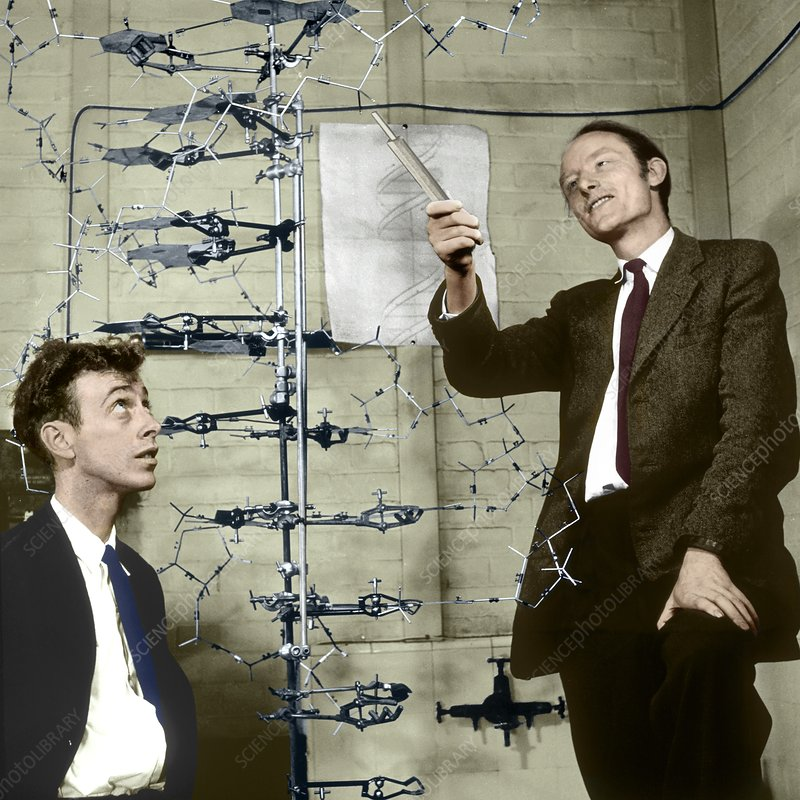
\includegraphics[scale=0.25]{images/screenshots/Watson and Crick.jpg}
    \end{minipage}%
    \begin{minipage}{.5\textwidth}
    \centering
         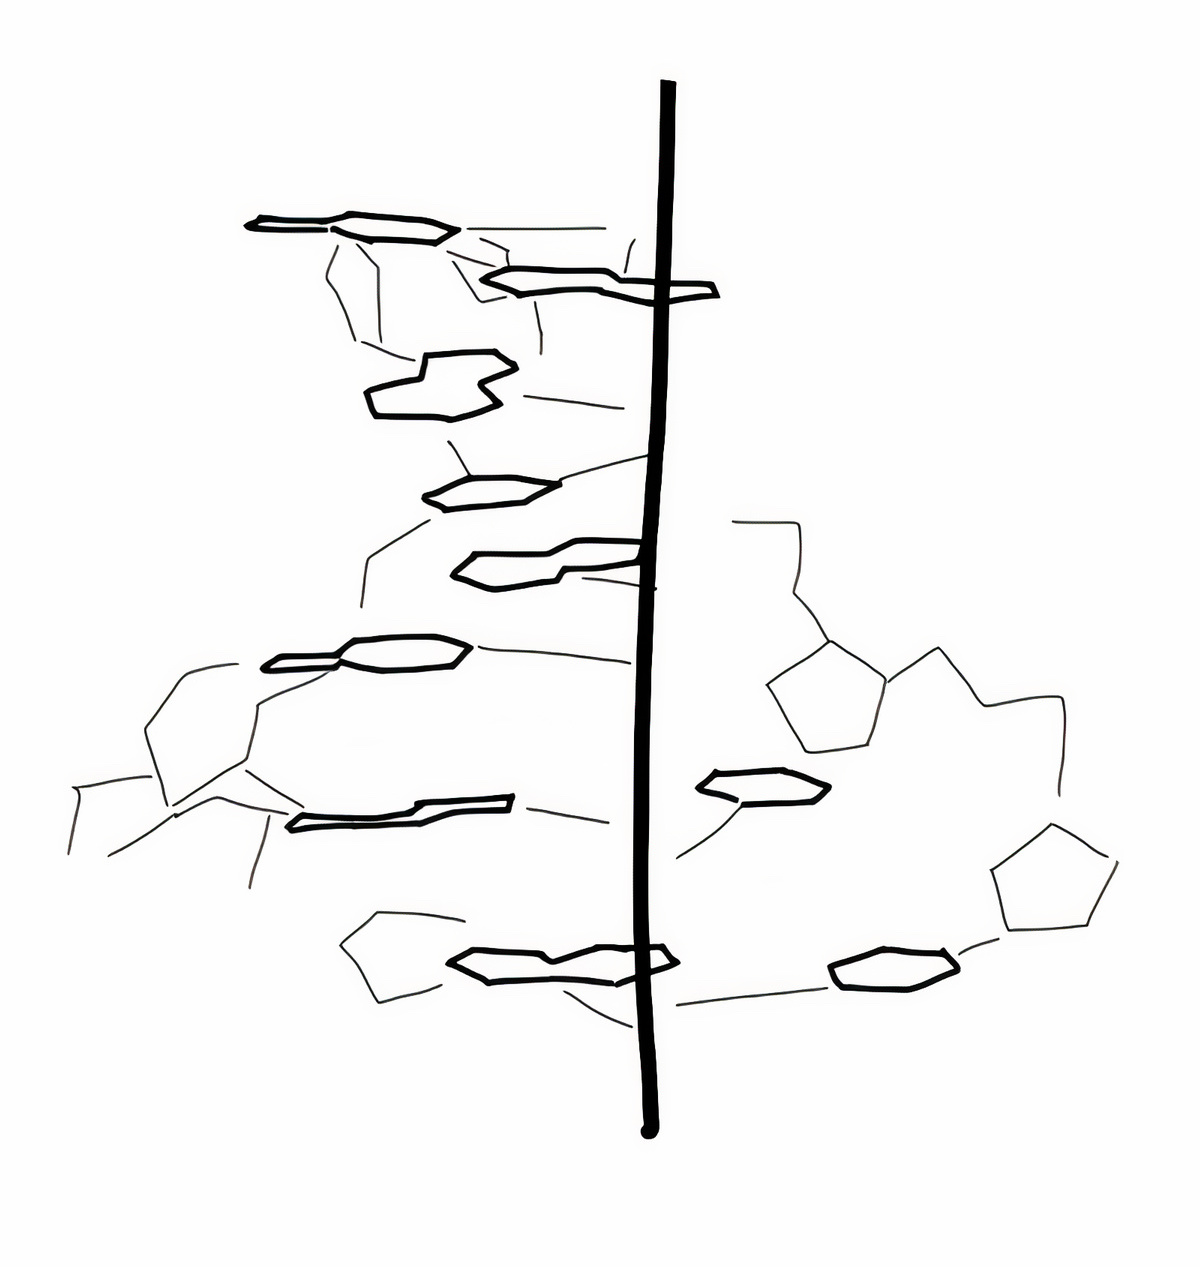
\includegraphics[scale=0.20]{images/sketches/rough_dna_structure.jpeg}
    \end{minipage}
\caption{The first graphic is the famous Watson and Crick image with their life-sized DNA model \cite{watson_and_crick}. The second graphic is a rough sketch of our initial design translation.}
\end{figure}
 
This propelled us to look for designs and styles inspired by the concept of Bioengineering rather than specific functional features. While exploring potential inspirations, we stumbled upon the famous image of Watson and Crick with a large life-sized 3-D model of the double helix structure of DNA. This gave us the silhouette for the design - our own unique plant-pot ensemble that would resemble the famous helical structure within our design philosophies and constraints. We wanted to design a Bioengineering-inspired exquisitely crafted visual delight. 
\pagebreak

\section{Design details}
\textit{Kindly refer to the Appendix (\ref{topic:technical_drawings}) for the technical drawings with the exact dimensions for each component described in this section.} 
\subsection{Overall Structure}

\begin{figure}[ht]
     \centering
     \begin{subfigure}[b]{0.4\textwidth}
         \centering
         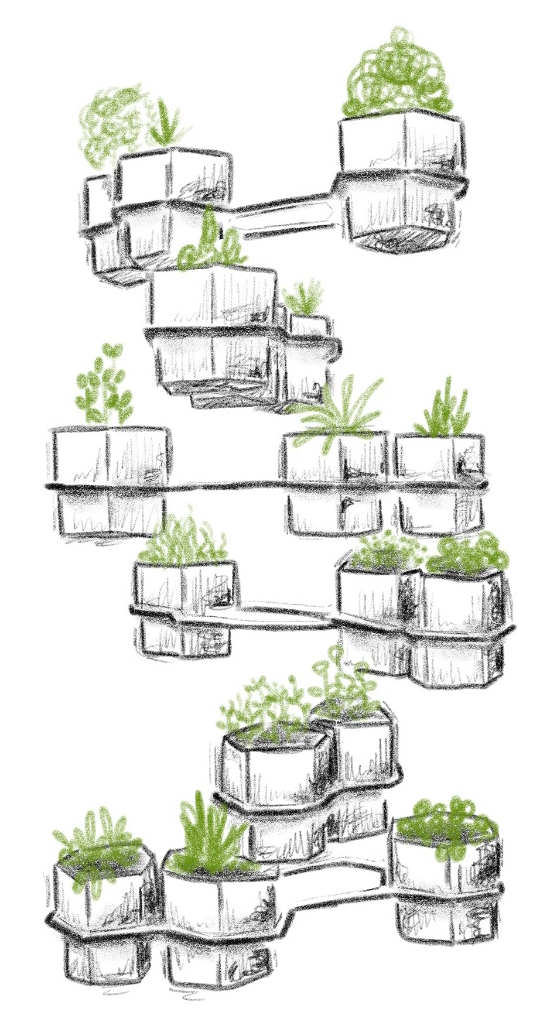
\includegraphics[width=\textwidth]{images/sketches/plant_pot_sketch.jpg}
         % \caption{Adenine Base Sketch}
         \caption{Well-drawn sketch of our design fully laid out.}
         \label{fig:whole_pot_sketch}
     \end{subfigure}
     \hfill
     \begin{subfigure}[b]{0.44\textwidth}
         \centering
         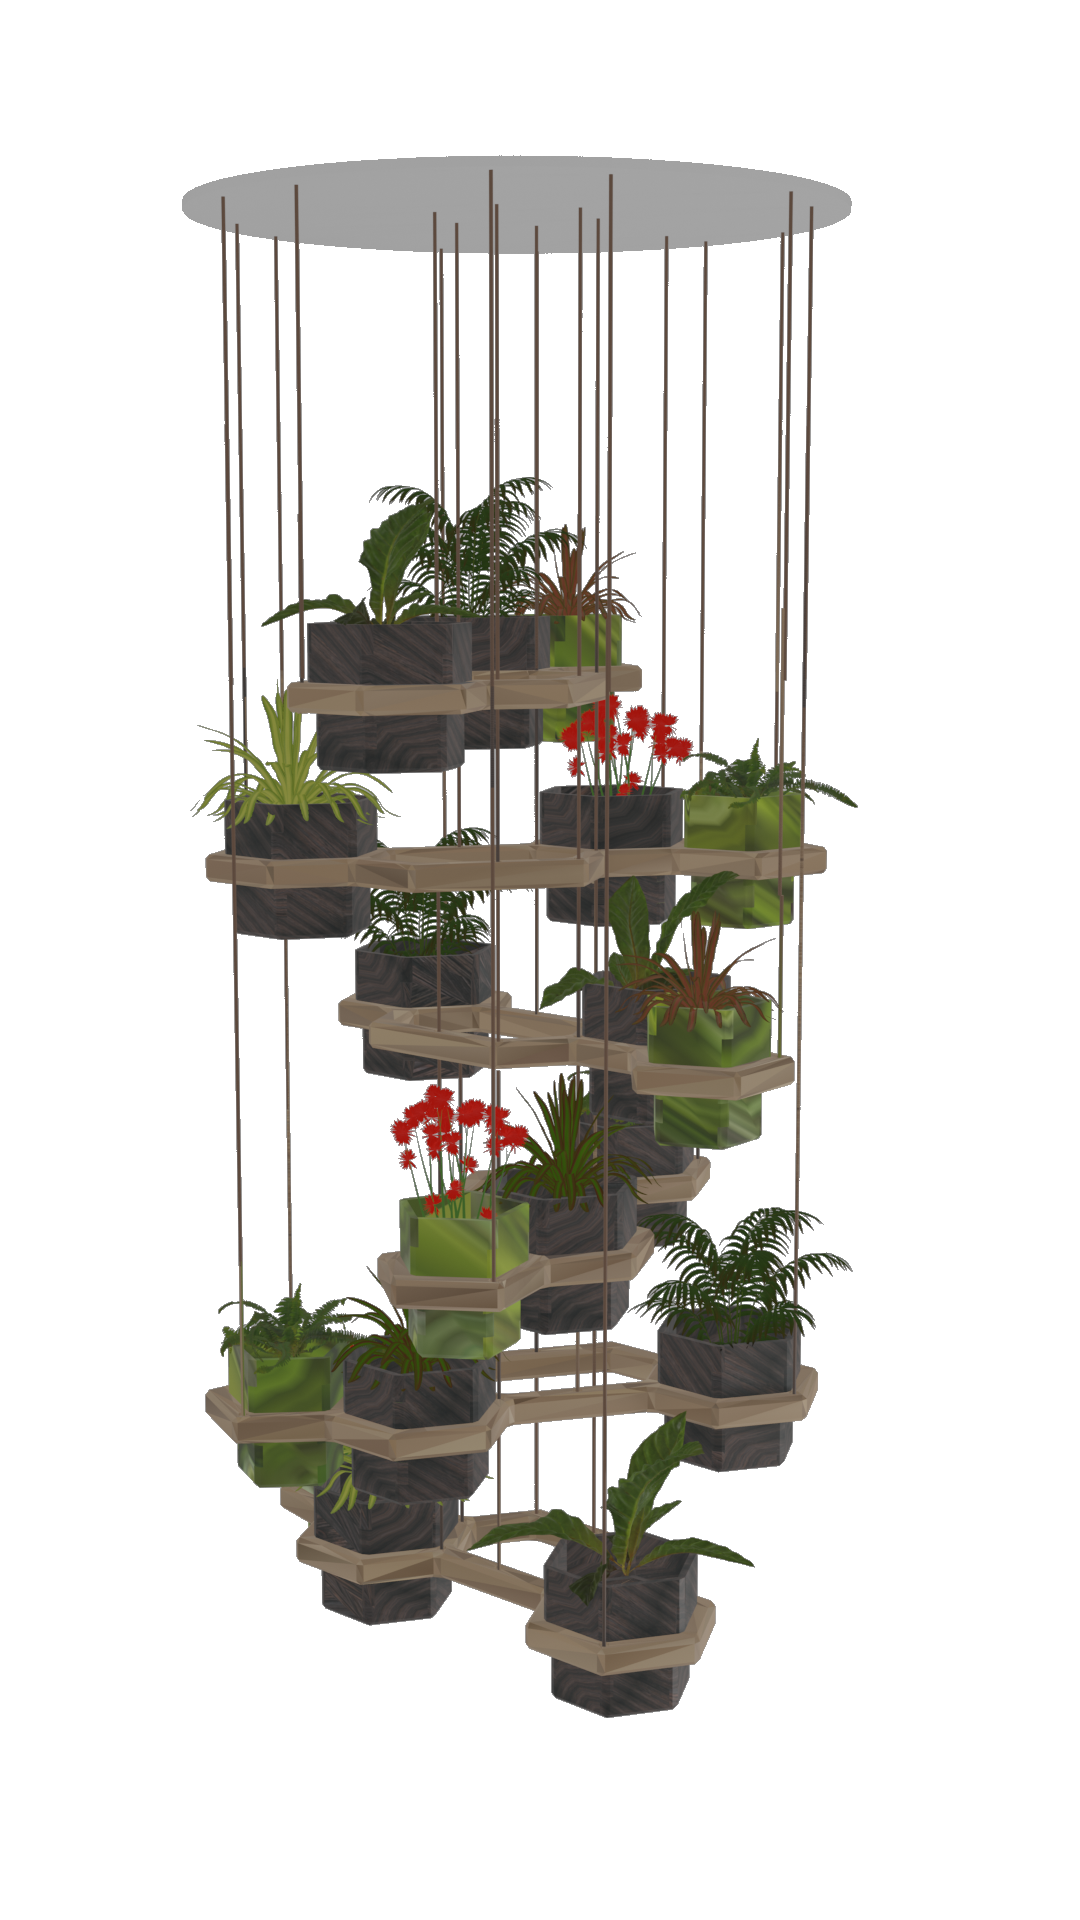
\includegraphics[width=\textwidth]{images/screenshots/plant_pot_transparent.png}
         % \caption{Base Pair Structure}
         \caption{Rendered image of our final design constructed in SolidWorks and shaded in Blender.}
         \label{fig:rendered_whole_structure}
     \end{subfigure}
     \caption{Sketch and render of the assembled final design with plants.}
\end{figure}

We designed a modern interpretation of the renowned DNA structure using pinewood. We re-imagined the nucleotide base pairs to create a unified structure, where each bond became a wooden edge and each atom served as a joint between them.

Furthermore, we designed the rings of nucleotide base pairs as slots to house the plant pots. This modular approach facilitated easy sliding in and out of the individual plant pots from the rings present in the base-pair structure. Each base pair can accommodate three plant pots: two in the two rings of a purine and one pot in the single ring of a pyrimidine.

To achieve a visible helical structure, we decided to stack base pairs at a \textbf{rotation of 60 degrees}, resulting in a complete turn of the helix every six base pairs. In addition, this arrangement prevented the upper pots from blocking the growth of plants on the lower base pairs.

\begin{figure}[ht]
     \centering
     \begin{subfigure}[b]{0.4\textwidth}
         \centering
         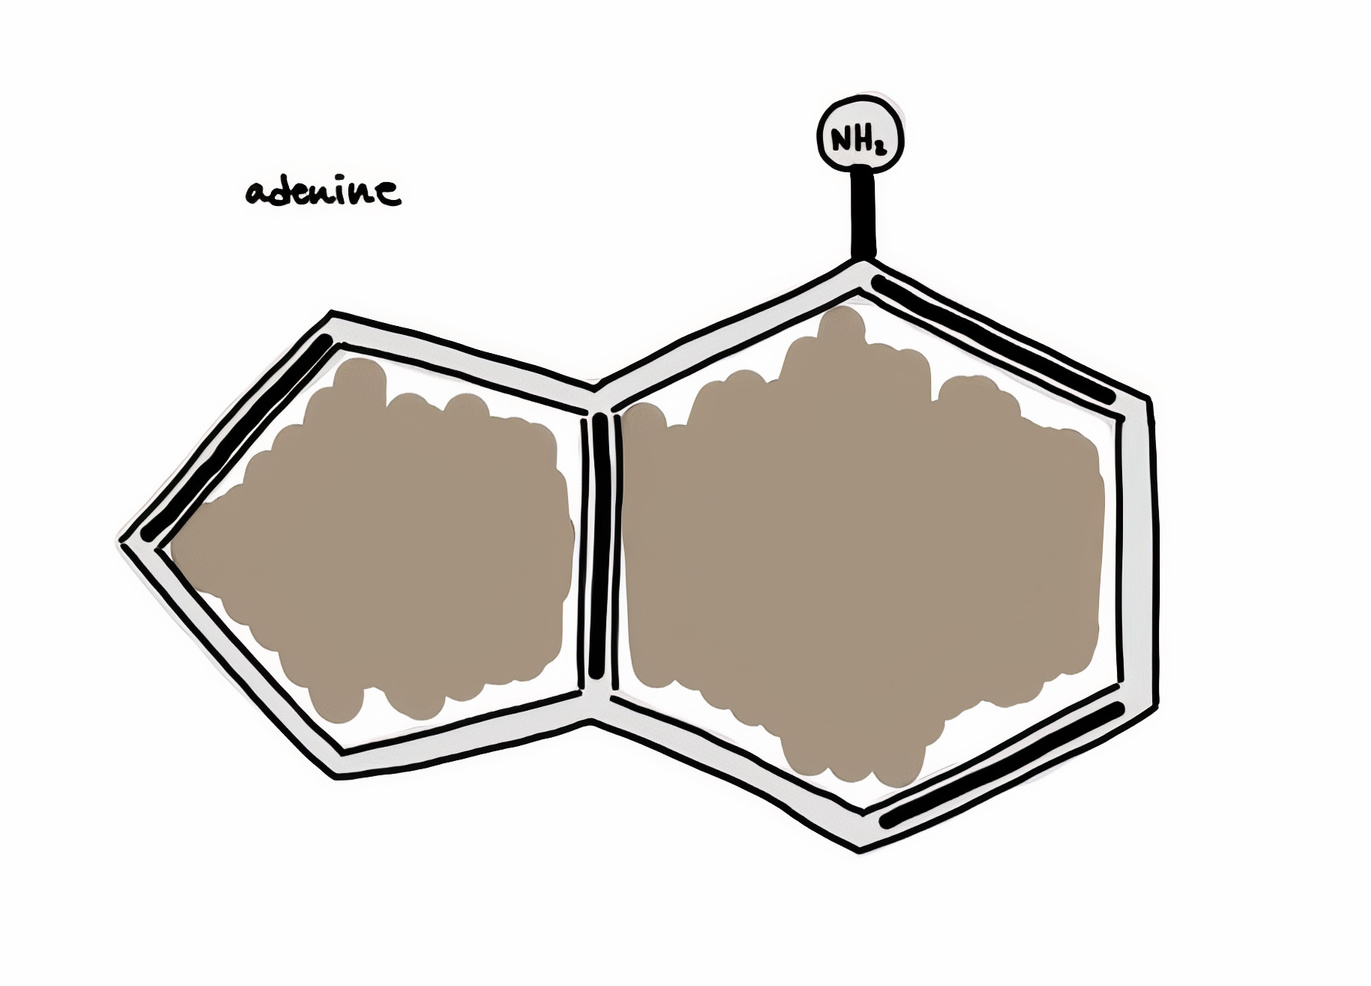
\includegraphics[width=\textwidth]{images/sketches/rough_plant_pot_placement.jpeg}
         % \caption{Adenine Base Sketch}
         \caption{Sketch drawn while brainstorming laying out where plant pots can be housed.}
         \label{fig:adenine_sketch}
     \end{subfigure}
     \hfill
     \begin{subfigure}[b]{0.55\textwidth}
         \centering
         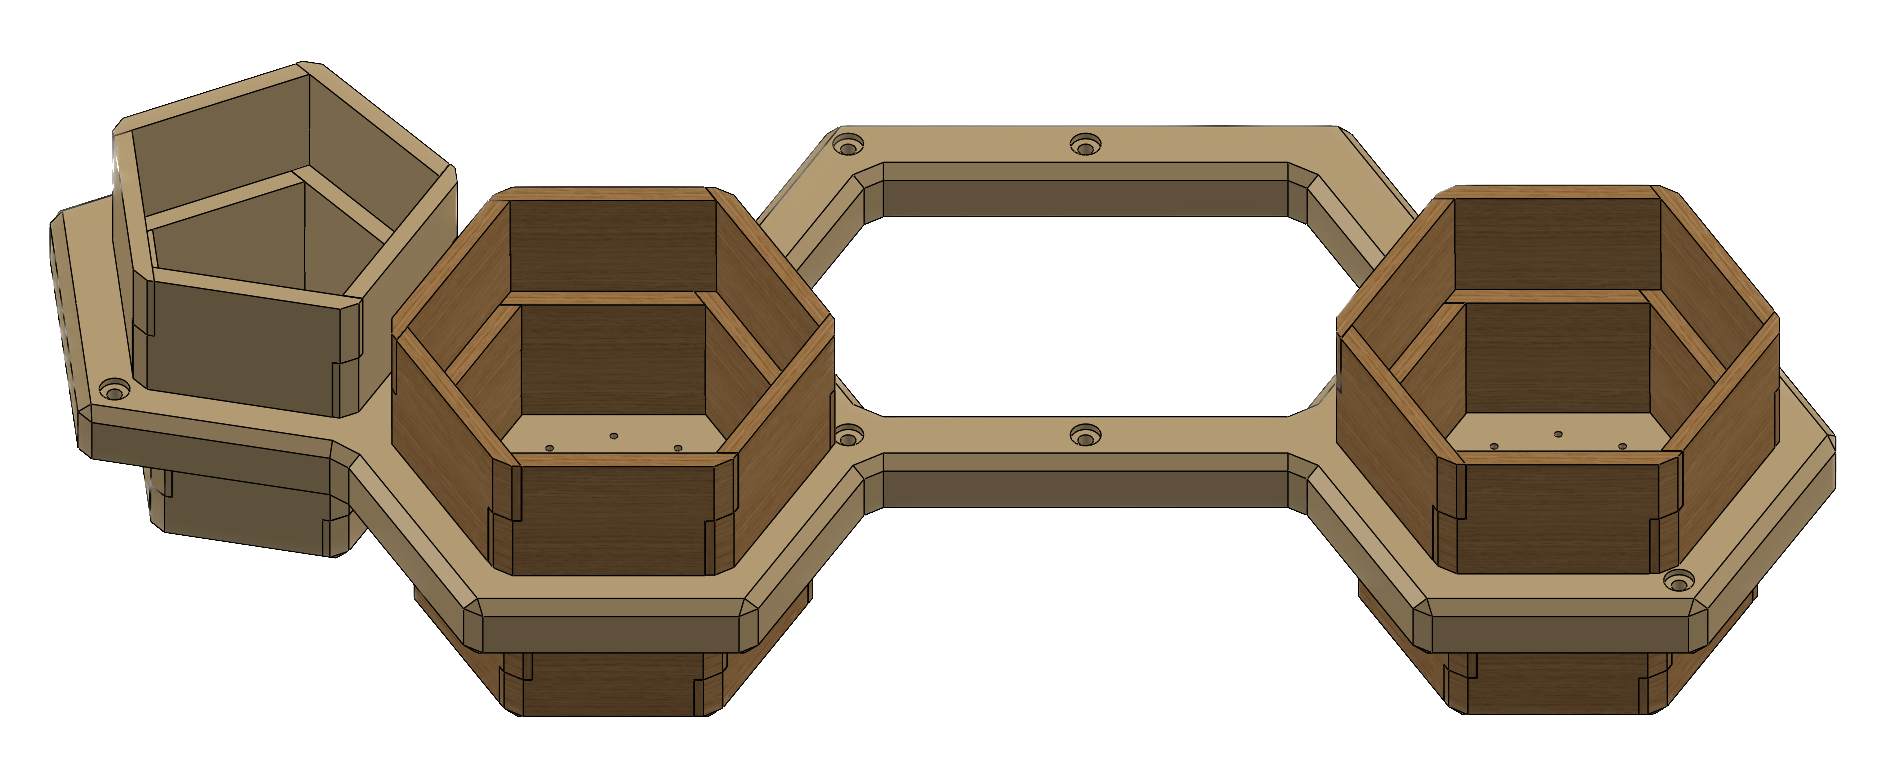
\includegraphics[width=\textwidth]{images/screenshots/bp_assembled.png}
         % \caption{Base Pair Structure}
         \caption{Rendered example of the unified base pair structure between Adenine and Thymine housing three pots in the three rings of the bases respectively.}
         \label{fig:bp_transparent}
     \end{subfigure}
     \caption{Sketch and render of the pots' positions in the base scaffolding.}
\end{figure}

To preserve the overall design aesthetic, we opted to maintain the hexagonal/pentagonal shape of the rings instead of rounding them from the inside. This choice resulted in an angular appearance throughout the entire design.

One of our key motivations was to maintain a minimalist and uncluttered design. With this in mind, we simplified the nitrogenous base pairs by eliminating all additional Hydrogen/Oxygen/Amine bonds from the side chains and keeping only the rings themselves. (The extruded amine group along with the etched representation of double bonds present in the Adenine sketch \ref{fig:adenine_sketch} is absent from the base-pair structure in Figure \ref{fig:bp_transparent})   

As is visible in Figure \ref{fig:rendered_whole_structure}, we also decided to suspend the structure from the ceiling using a ceiling mount and 4 mm sisal rope strands, rather than supporting the structure from the ground.
This ensured the balance of our modular ensemble and, at the same time, reduced structural complexity, number of parts used and total weight of the overall structure.


\label{para:max_stress}
We made sure that the base scaffold was robust enough to support the weight of the plant pots along with the soil and water during static stress test simulations (Appendix \ref{screenshot:stress_test_image}).

We determined that our composition (six base pairs or more) could be suspended using a total of 18 sisal ropes. This was made possible by multiple inner string holes aligning perfectly from top to bottom and therefore sharing individual sisal strands.

% Stress Test Image
\begin{figure}[!ht]
    \centering
    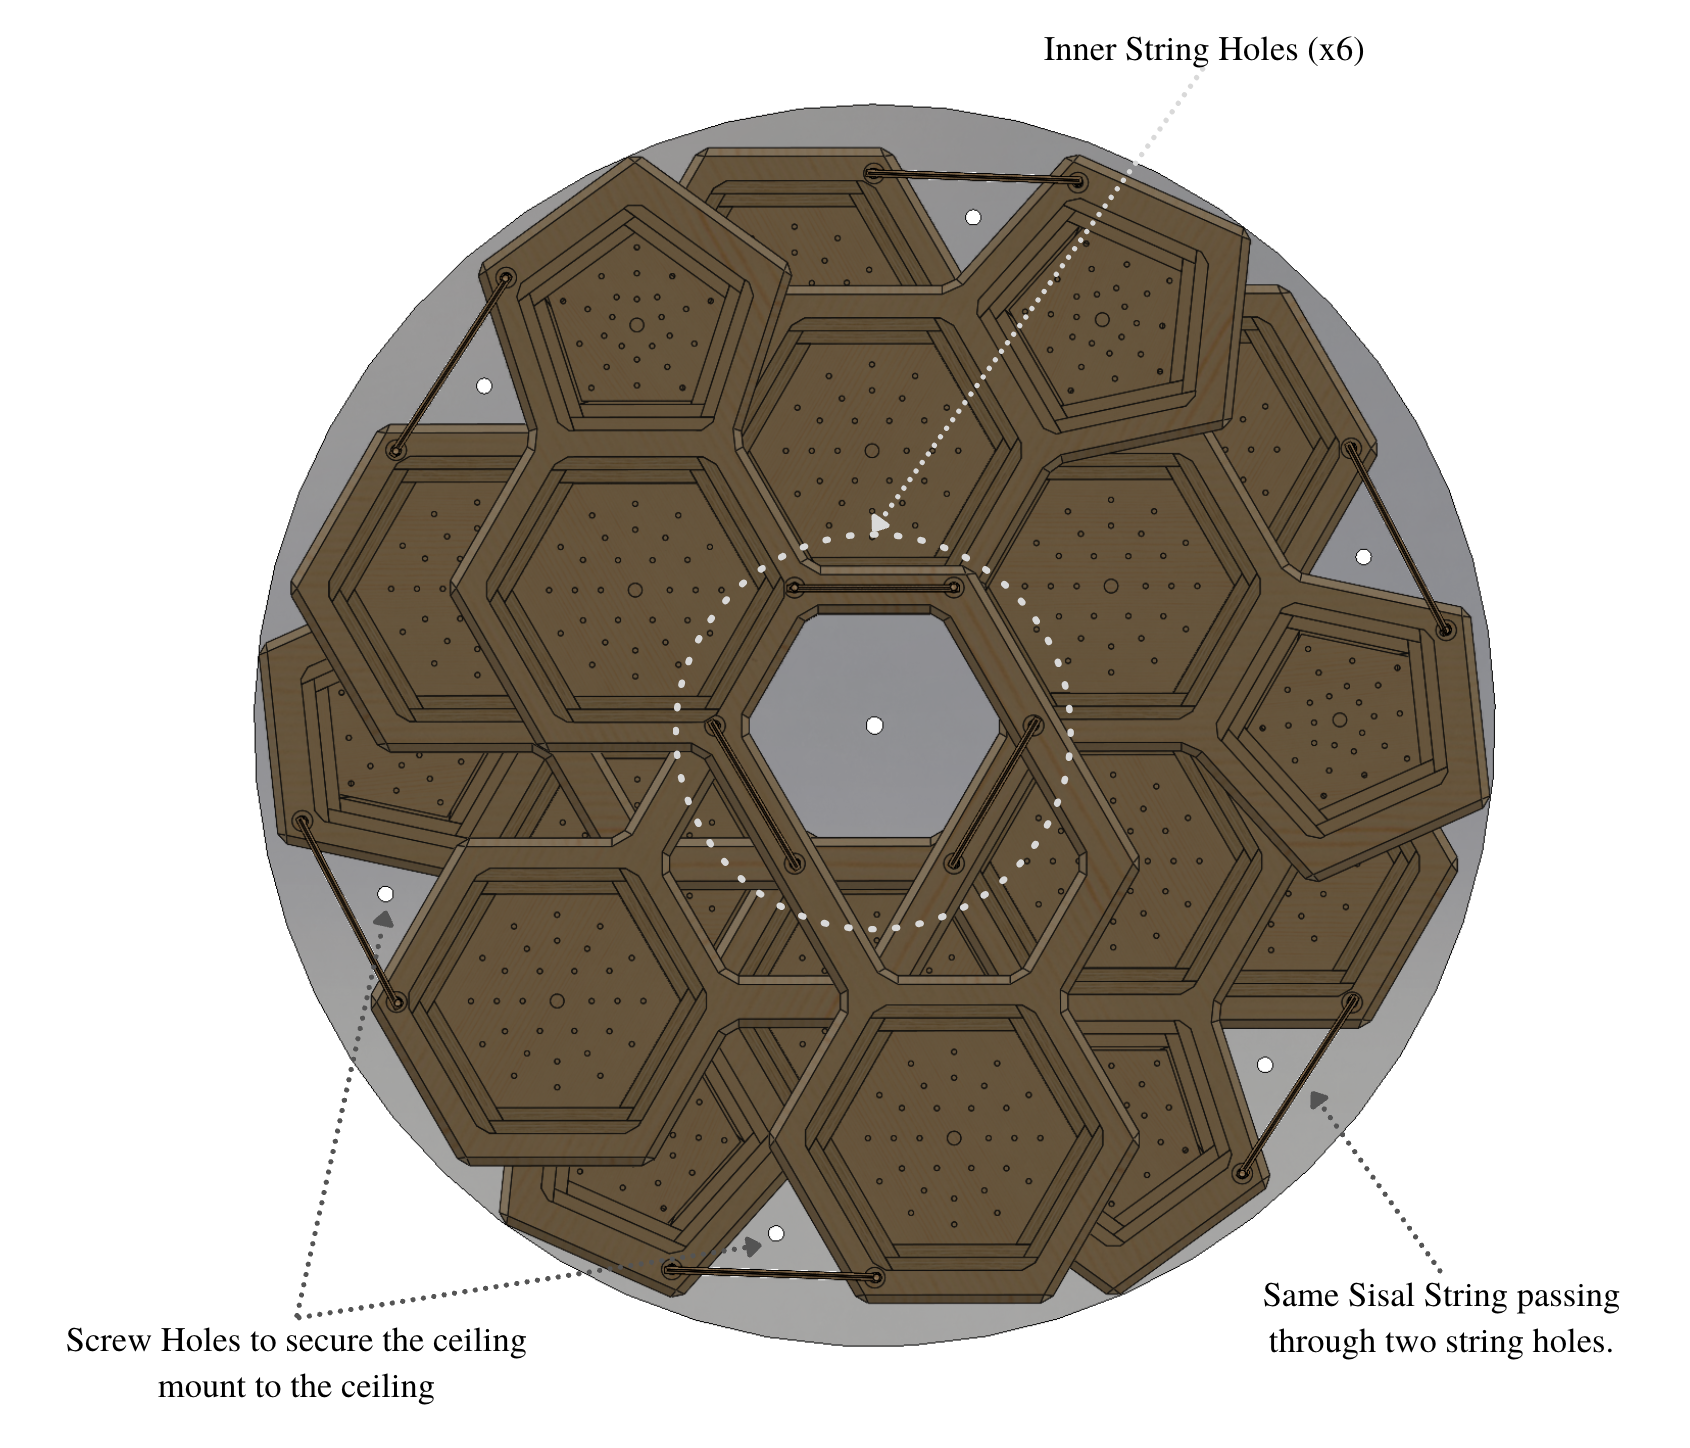
\includegraphics[width=0.7\textwidth]{images/screenshots/ceiling_mount_3d.png}
    \caption{Top view of the Ceiling Mount. The smaller 6 mm holes (18x) are where the sisal strings will be attached. The larger 9 mm holes (7x) are screw holes that would be used to fasten the mount to the ceiling.}
    \label{fig:ceiling_mount_annotated}
\end{figure}

To prevent screwing 18 hooks into the ceiling, we designed a simple metallic ceiling mount, to which the ends of all sisal strings can be tied. The use of only seven ceiling hooks simplifies the installation procedure. We designed the ceiling mount in such a way that 9 individual ropes can be used to suspend the entire structure with one rope passing through two holes from the top (as visible in the top view of the ceiling mount in Figure \ref{fig:ceiling_mount_annotated}). 

\pagebreak
\subsection{Plant Pots}
The design of an individual plant pot was a crucial element in the overall process. Since we had two different types of slots - one hexagonal and one pentagonal - a pinewood pot was designed for each of these two slots.

One of the most obvious concerns when designing the pots out of wood was to avoid accelerated decay by soil and water. To prevent this, we found a highly reliable wood polymer sealant that could be coated on the entire surface of the pots (inside and outside) to create a protective seal against water damage.

As visible in the images \ref{fig:hex_pot} and \ref{fig:pent_pot}, the plant pot has two design segments - the upper segment which has a bigger diameter and proportionally bigger volume and will sit on top of the base pair; and the lower segment which has a smaller diameter and can thus slide into the base pair ring enclosure. The difference in diameters was deliberately chosen in order for the plant pot to easily slide into and rest on the rings of the base pairs. 

As shown in Figure \ref{fig:pent_pot_half}, the lower segment of the plant pot houses a small water chamber which contains the excess water from watering and is separated from the main body of the pot via a secondary wooden bottom. 
We also added the option to install a braided cotton wick that runs from the soil to the water chamber through the larger hole to maintain the soil's moisture. We only chose a single wick to ensure that the soil does not become overly damp which may have an adverse effect on the plant.
\clearpage
\begin{figure}[ht]
     \centering
     \begin{subfigure}[b]{0.45\textwidth}
         \centering
         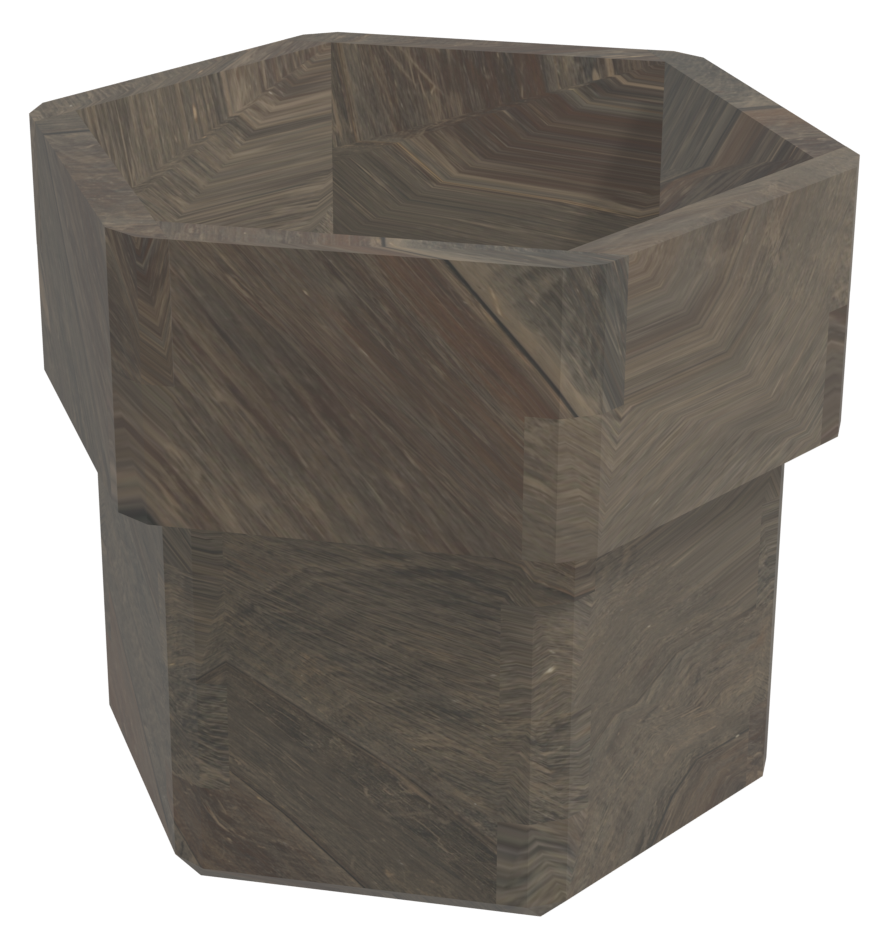
\includegraphics[width=\textwidth]{images/screenshots/hexagonpot.png}
         % \caption{Adenine Base Sketch}
         \caption{3d Render of the plant pot for the \textbf{hexagonal ring} for the nitrogenous base.}
         \label{fig:hex_pot}
     \end{subfigure}
     \hfill
     \begin{subfigure}[b]{0.43\textwidth}
         \centering
         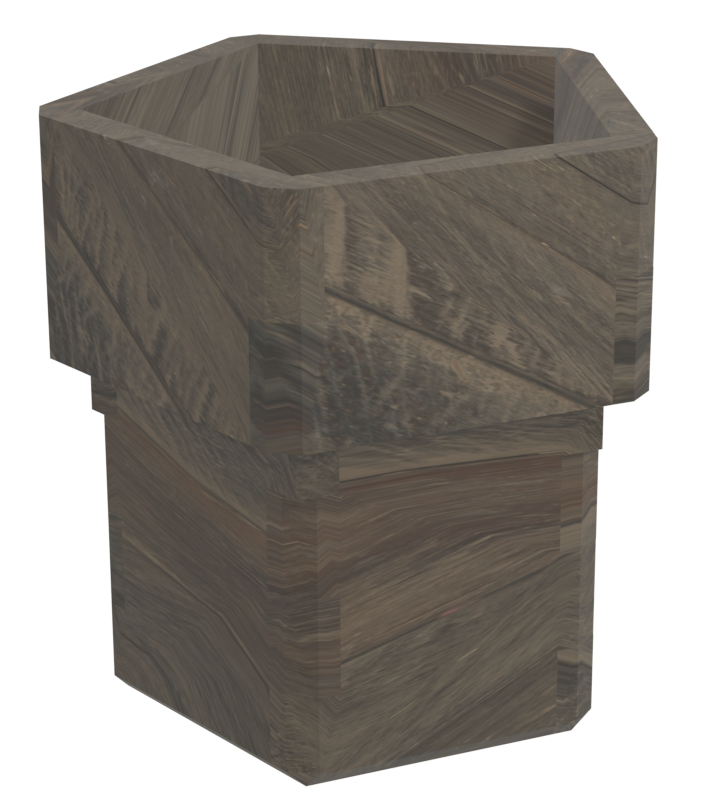
\includegraphics[width=\textwidth]{images/screenshots/pentagonpot.png}
         % \caption{Base Pair Structure}
         \caption{3d Render of the plant pot for the \textbf{pentagonal ring} for the nitrogenous base.}
         \label{fig:pent_pot}
     \end{subfigure}
     \caption{Blender produced images, reflecting the wooden texture of the design.}
\end{figure}
\begin{figure}[H]
     \centering
     \begin{subfigure}[b]{0.65\textwidth}
         \centering
         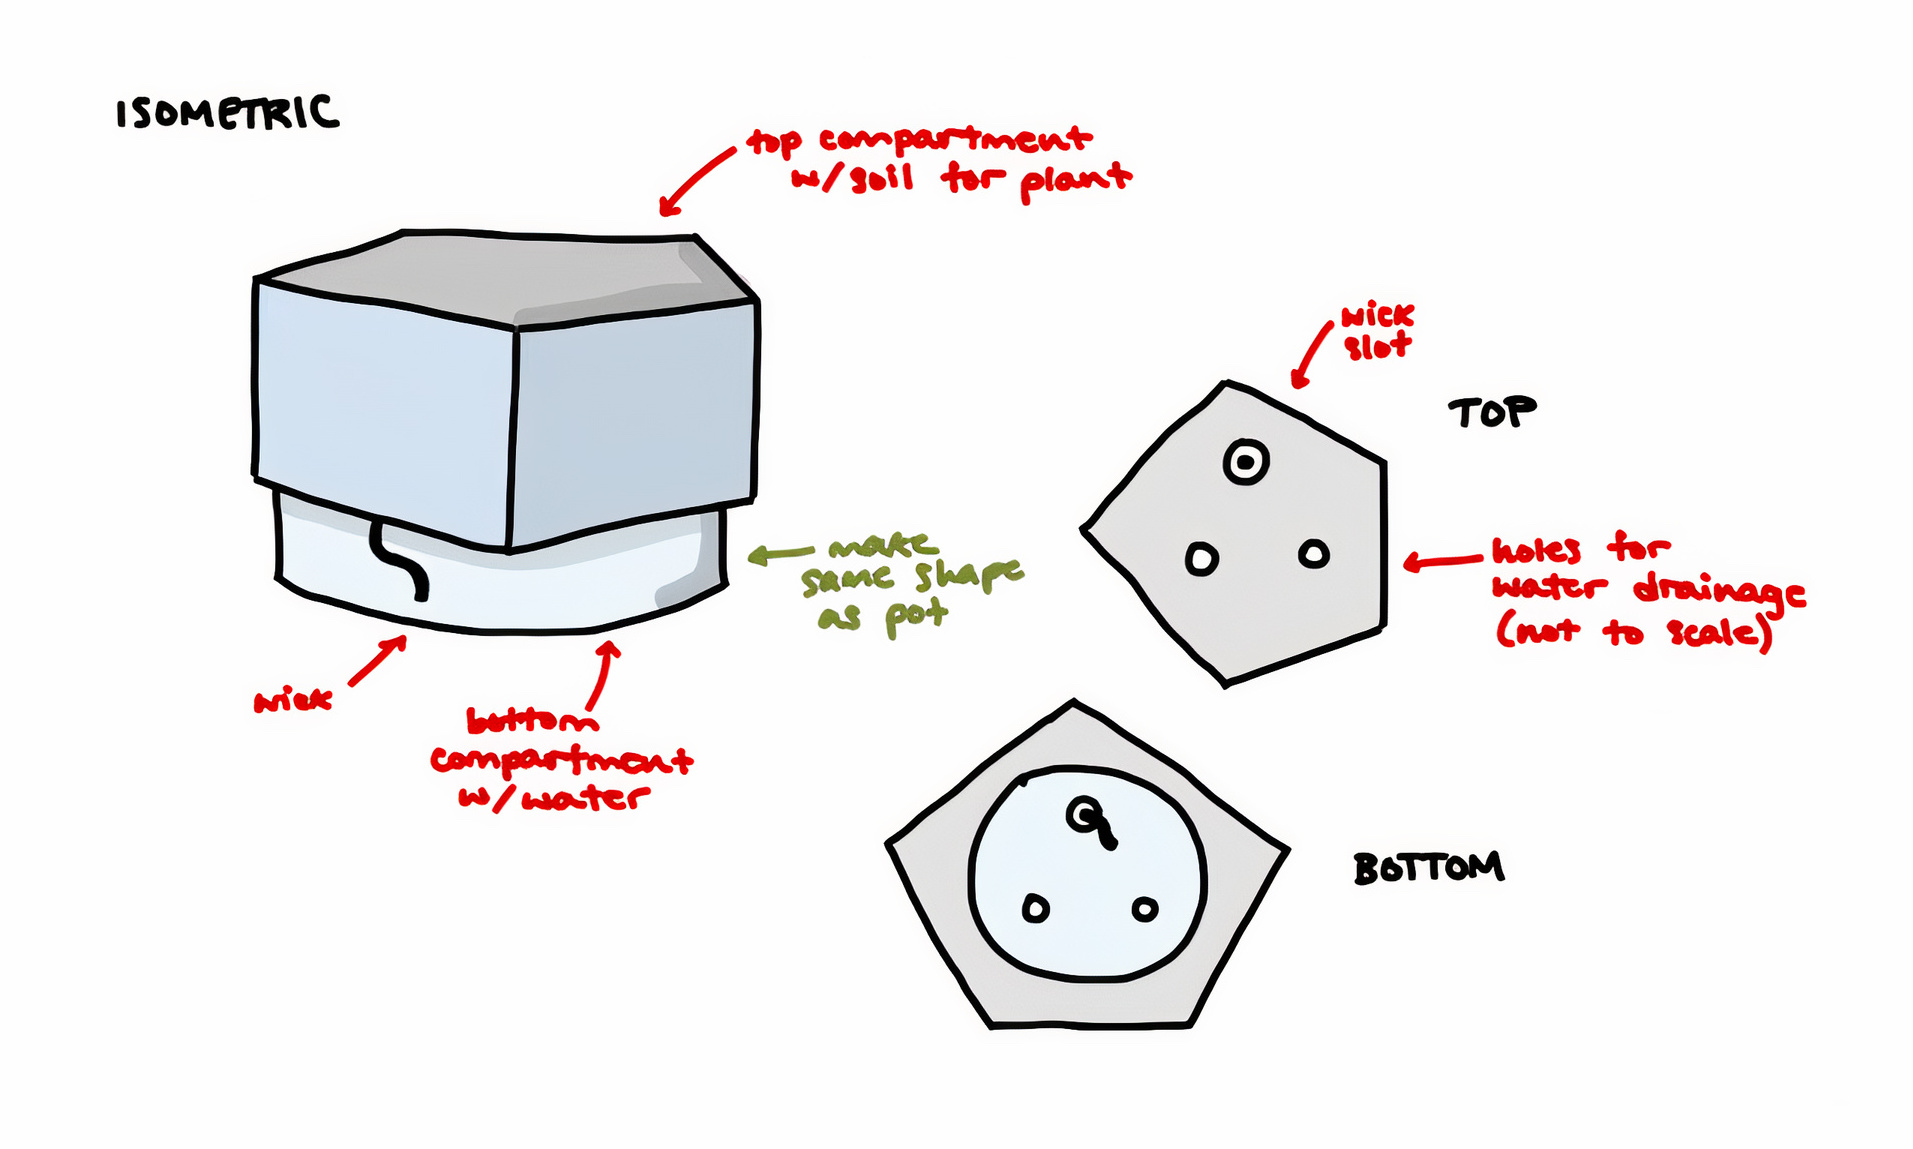
\includegraphics[width=\textwidth]{images/sketches/initial_plant_pot_idea.jpeg}
         \caption{Sketch drawn during the design phase displaying our initial design idea for the plant pot. The circular lower part design was later superseded by a polygonal shape. This sketch also shows where the wicking mechanism.}
         \label{fig:initial_plant_pot_sketch}
     \end{subfigure}
     \hfill
     \begin{subfigure}[b]{0.3\textwidth}
         \centering
         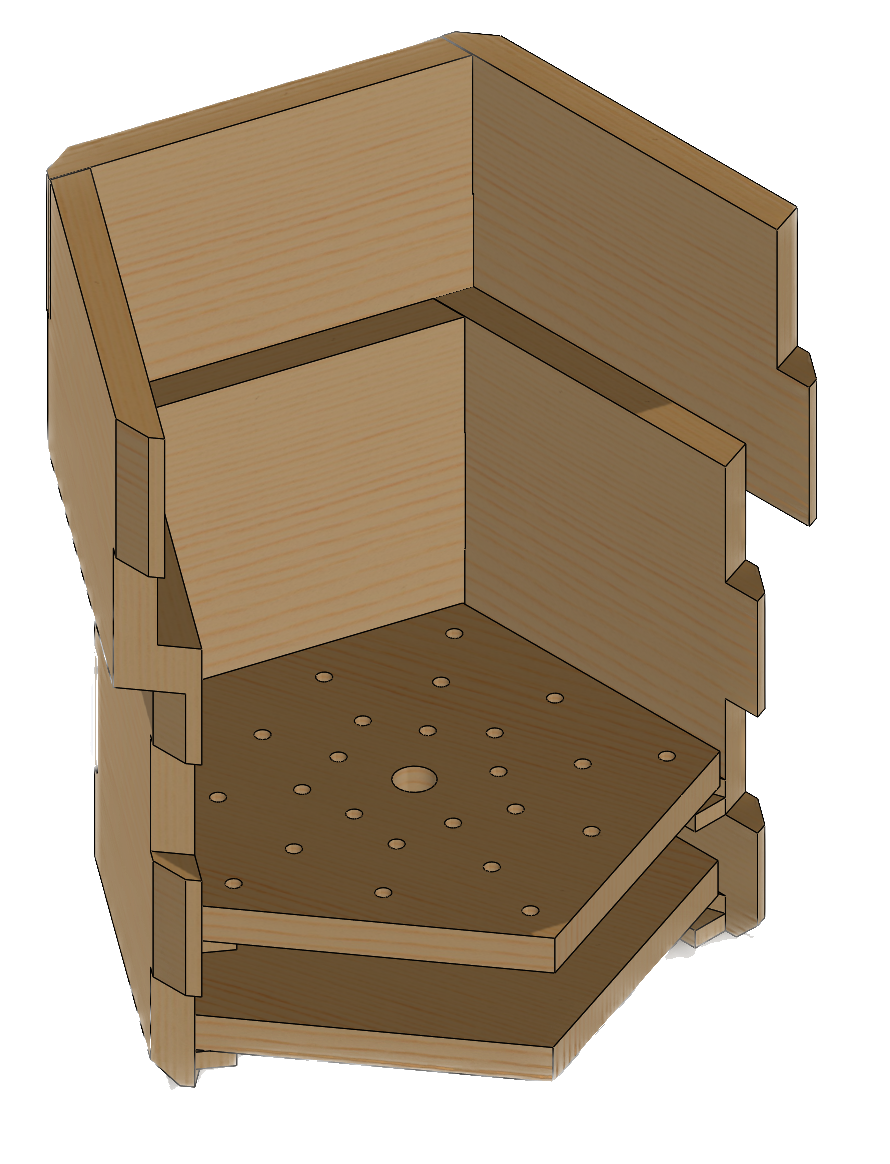
\includegraphics[width=\textwidth]{images/screenshots/pent_pot_half_transparent.png}
         % \caption{Base Pair Structure}
         \caption{An open 3-D render of the plant pot displaying the inner bottom separating the soil and water chamber. The smaller holes allow excess water to drain into the water chamber. The larger hole is present to encapsulate a wick from the soil to the water chamber.}
         \label{fig:pent_pot_half}
     \end{subfigure}
     \caption{Sketch and render of the pot's inner design.}
\end{figure}

\newpage
\subsection{Bill of Materials}\label{topic:bill_of_materials}
\begin{table}[ht]
  \begin{center}
  \begin{minipage}{500pt}
  \caption{Bill of all materials required for manufacturing and assembly}\label{tab1}
  \begin{tabular}{m{2.5em}  m{8em} m{6em}  m{6em}  m{10em} m{4em}} 
  % {@{\extracolsep{\fill}}lcccccc@{\extracolsep{\fill}}}
    \toprule
   Serial No. & Material & Quantity & Price/Base Pair (GBP) & Price/Entire Structure (GBP) & Purchase Link\\
    \midrule
        1. & Pine Wood Panel\footnote{ 1/4 of a 33 x 270 x 4500mm panel; wastage included} & 0.020 m$^{3}$  & 3.00 & 18.00 & \href{http://www.chilterntimber.co.uk/product/laminated-pine-board-33-x-4500mm-x-various-widths/}{link}\\
        
        2. & Clippers & 60 units & 1.80 & 9.00 & 
        \href{https://www.alibaba.com/product-detail/Custom-stainless-steel-fitting-cable-rail_1600802307080.html}{link}\\
        3. & Sisal String & 30 m & 0.13 & 0.75 & \href{https://www.alibaba.com/product-detail/100-Natural-sisal-Rope-1mm-50mm_1600765012684.html}{link}\\
        4. & Pure Tung Oil & 1 Litre\footnote{Total Area of wood per base pair (including three pots) = 0.9 $m^{2}$ * 6 Base Pairs = $~5.4 m^{2}$ of total coating area. 1 Litre of tung oil would give us ~3–4 coats of the entire area of wood.} & 2.12 & 12.74 & \href{https://www.amazon.co.uk/Pure-Tung-Oil-Bestwood-500ml/dp/B009YKW9LU?source=ps-sl-shoppingads-lpcontext&ref_=fplfs&psc=1&smid=A2E8NZBD2EH78J}{link}\\
        5. & Wood Glue & 0.4 Kg & 0.06 & 0.36 & \href{https://www.alibaba.com/product-detail/Japanese-JIS-standard-white-glue-wood_1600741536039.html?spm=a2700.galleryofferlist.0.0.70d07a4bfT8qAG}{link}\\
        
        6. &  Aluminium Sheet\footnote{750 x 750 x 2 mm sheet; wastage included.} & 1 sheet  & - & 27.07 & \href{https://www.1stchoicemetals.co.uk/product/2mm-3/}{link}\label{bill:alumninium_sheet}\\
        
        7. & Sleeve Anchor & 7 units & - & 9.03 & \href{https://www.hilti.co.uk/c/CLS_FASTENER_7135/CLS_SLEEVE_ANCHORS_NAIL_ANCHORS_7135/r3955}{link}\\
        8. & Wick & 1 m & 0.04 & 0.68 & \href{https://www.alibaba.com/product-detail/Macrame-Twist-Braided-Cord-100-Macrame_1600204884923.html?}{link}\\
        \midrule
        & & & Total & 78 GBP\\
    \bottomrule
  \end{tabular}
  \end{minipage}
  \end{center}
  \end{table}

\section{Discussion}
\subsection{Choice of materials}\label{topic:choice_of_materials}
\subsubsection{Wood}
In our material selection process, we considered criteria for simplicity, sustainability, and cost-effectiveness. Our objective was to explore alternatives to conventional plastics while prioritising the aesthetics of the texture. With these goals in mind, we ultimately chose pinewood as the primary material for our design. We selected pinewood over oak or other common wood counterparts due to the following advantages it offers:

\begin{itemize}
    \item Versatility: Pinewood is a lightweight wood, which facilitates ease of workmanship and handling during the manufacturing process.
    \item Cost: Pinewood is a cost-effective alternative as it is naturally grown in the UK and is relatively inexpensive.
    \item Aesthetics: After polishing, pinewood exhibits a visually pleasing texture.
\end{itemize}

\textbf{Redwood} or \textbf{Cedar} could also be considered as alternatives. These woods are harder, which can provide increased durability and strength. However, they come with certain trade-offs, such as increased weight of the structure and significantly higher price.


\subsubsection{Biopolymer}
Upon finalising the wood selection, it became crucial to determine the appropriate biopolymer sealant to prevent the wood from getting damp. We extensively explored various options, including varnish, oils, resin, beeswax, polyurethane, and more. Our primary focus was to identify a natural and non-toxic sealant that would ensure the absence of soil and plant toxicity. Consequently, we eliminated polyurethane due to its plastic nature, which could potentially lead to the bioaccumulation of microplastics in the plants. We also took cost-effectiveness into consideration.

We ultimately selected \textbf{pure tung oil} as the best overall wood coat\cite{tung_oil}. This choice was driven by its natural composition, biodegradability, and non-toxic properties, as well as its excellent water-repellent properties. Furthermore, \textbf{pure tung oil} provides an aesthetic 'wet' looking finish. It is important to note a few potential drawbacks - relatively long drying time, ranging from 24 to 32 hours, and the presence of a mild odour for a few days after application. While not crucial, different shades of polish could also be applied to different pots for a much more vibrant design as present in \ref{fig:rendered_whole_structure}\footnote{This step is optional, and we haven't included this in the Assembly or Bill of Materials.}.

\subsection{Manufacturing}
\subsubsection{Plant Pot Components}
\begin{figure}[!ht]
     \centering
     \begin{subfigure}[b]{0.2\textwidth}
         \centering
         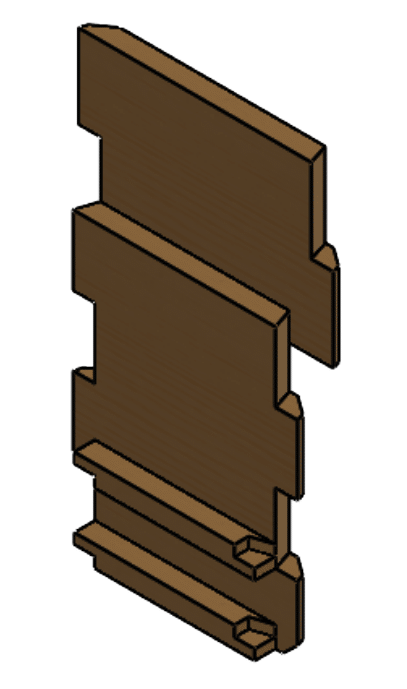
\includegraphics[width=\textwidth]{images/screenshots/ind_pot_comp/Pentagonal side-1.png}
         \caption{Side Part}
         \label{fig:pent_pot_side_part}
     \end{subfigure}
     \hfill
     \begin{subfigure}[b]{0.35\textwidth}
         \centering
         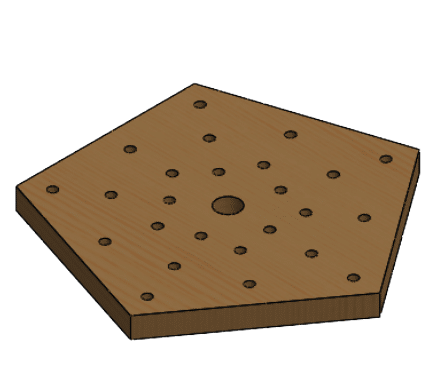
\includegraphics[width=\textwidth]{images/screenshots/ind_pot_comp/Pentagonal false bottom-1.png}
         \caption{Inner Bottom Part}
         \label{fig:pent_pot_inner_bottom}
     \end{subfigure}
     \begin{subfigure}[b]{0.35\textwidth}
         \centering
         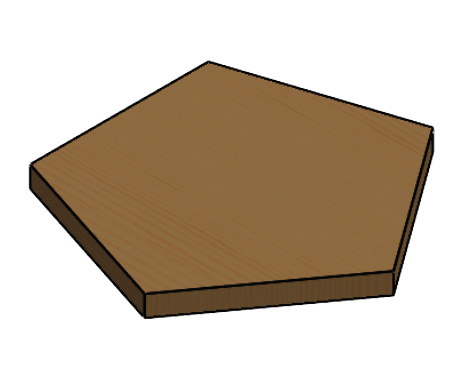
\includegraphics[width=\textwidth]{images/screenshots/ind_pot_comp/Pentagonal pot bottom-1.png}  
         \caption{Outer Bottom Part}
         \label{fig:pent_pot_outer_bottom}
     \end{subfigure}
     \caption{3-d Render of the three individual components required to be manufactured via CNC milling mentioned in the section \ref{topic:CNC_Milling}. \textit{*Note: these components are required for the pentagonal pot. The individual components required for the hexagonal pots with the exact dimensions are present in the technical drawings - \ref{technical_drawing:hex_pot_side_part}, \ref{technical_drawing:hex_pot_inner_bottom}, \ref{technical_drawing:hex_pot_outer_bottom}.}}
     \label{fig:ind_pot_components}
\end{figure}

The plant pots are composed of three individual components - a side part, the inner bottom, and the outer bottom - as displayed in Figure \ref{fig:ind_pot_components}. \label{topic:CNC_Milling} These parts are deliberately designed in such a way that they can easily be pieced together; \textit{similar to assembling Lego blocks}. 
\label{topic:CNC_milling_side_part}The side part (figure \ref{fig:pent_pot_side_part}) needs to be CNC milled from one side, then flipped around and milled from the other side. A negative mould would ensure the piece is stable while milling from the other side. 

For the Inner Bottom Part (figure \ref{fig:pent_pot_inner_bottom}) and the Outer Bottom Part (figure \ref{fig:pent_pot_outer_bottom}), the pieces can also be manufactured using laser cutting as it might be simpler and less expensive. 

\textit{Since these methods result in wasted wood, the additional wood required is also accounted for in the bill of materials (section \ref{topic:bill_of_materials}).} 

\hspace{0.1cm}

Components required for an individual \textbf{Pentagonal Pot}:
\begin{itemize}
    \item 5 * Pentagonal Side Part (figure \ref{technical_drawing:pent_pot_side_part})
    \item 1 * Pentagonal Inner Bottom (figure \ref{technical_drawing:pent_pot_inner_bottom})
    \item 1 * Pentagonal Outer Bottom (figure \ref{technical_drawing:pent_pot_outer_bottom})
\end{itemize}

Components required for an individual \textbf{Hexagonal Pot}:
\begin{itemize}
    \item 5 * Hexagonal Side Part (figure \ref{technical_drawing:hex_pot_side_part})
    \item 1 * Hexagonal Inner Bottom (figure \ref{technical_drawing:hex_pot_inner_bottom})
    \item 1 * Hexagonal Outer Bottom (figure \ref{technical_drawing:hex_pot_outer_bottom})
\end{itemize}

\textbf{Quantity of Plant Pots} required for the entire structure:
\begin{itemize}
    \item 2 * Hexagonal Pots / Base Pair * 6 Base Pairs = 12 Hexagonal Pots for 6 Base Pairs.
    \item 1 * Pentagonal Pots / Base Pair * 6 Base Pairs = 6 Pentagonal Pots for 6 Base Pairs.
\end{itemize}
\textit{The quantities can be changed depending on the number of base pair scaffolds used for the overall structure based on the above calculations. }

\subsubsection{Base Pair Scaffolding}
\begin{figure}[ht]
    \centering
    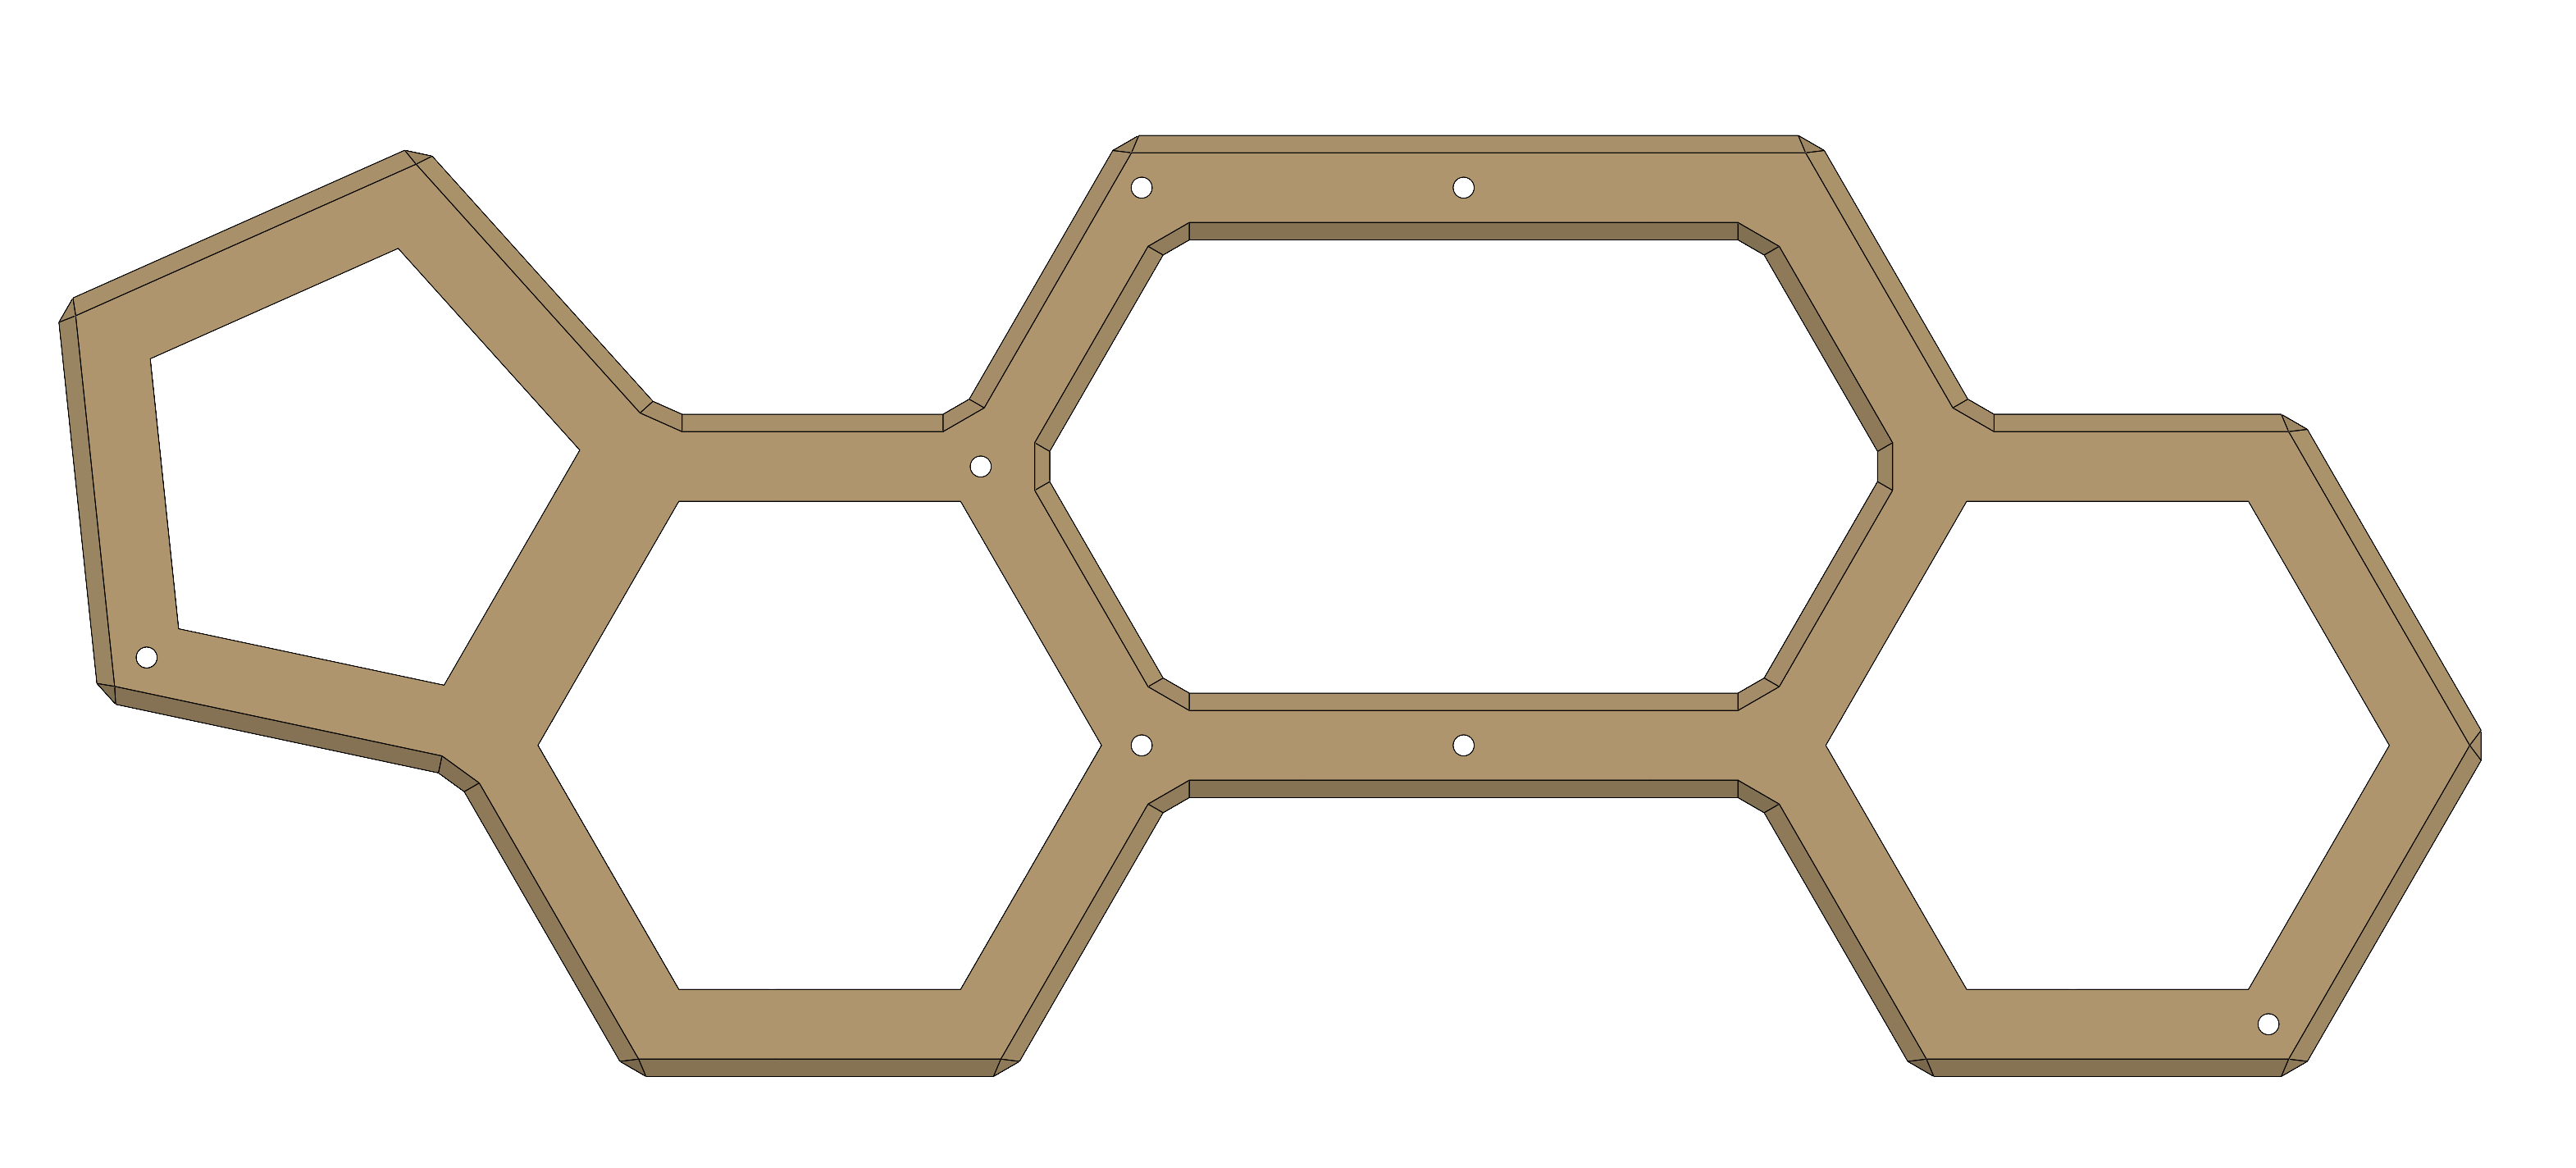
\includegraphics[width=0.5\textwidth]{images/screenshots/bp_transparent.png}
    \caption{Top view of the Base-Pair scaffolding that needs to be CNC milled. The string holes can be drilled by the CNC mill.}
    \label{topview:basepair}
\end{figure}

The base pair scaffolding, where the pots will rest, can also be manufactured via two-step CNC milling (similar to the process described for the side part of the plant pot in section \ref{topic:CNC_milling_side_part}). First, the large flat side is CNC milled from a wood slab; then, the part is flipped and placed into a negative mold, in order to mill the opposite side. (\textit{*This is achieved as there is no overhang present on those faces}). As per our initial design choice, \textbf{6 copies} of the same scaffolding are required for the entire structure.

\subsubsection{Ceiling Mount}
The Ceiling Mount (figure \ref{technical_drawing:ceiling_mount}) can be manufactured by cutting a single sheet of aluminium (Bill of Materials Section \ref{bill:alumninium_sheet}) and drilling holes of appropriate size. The edges would need to be deburred afterwards to prevent damage to the Sisal strands.

\pagebreak
\subsection{Assembly}
\subsubsection{Individual Plant Pots}
\begin{figure}[ht]
    \centering
    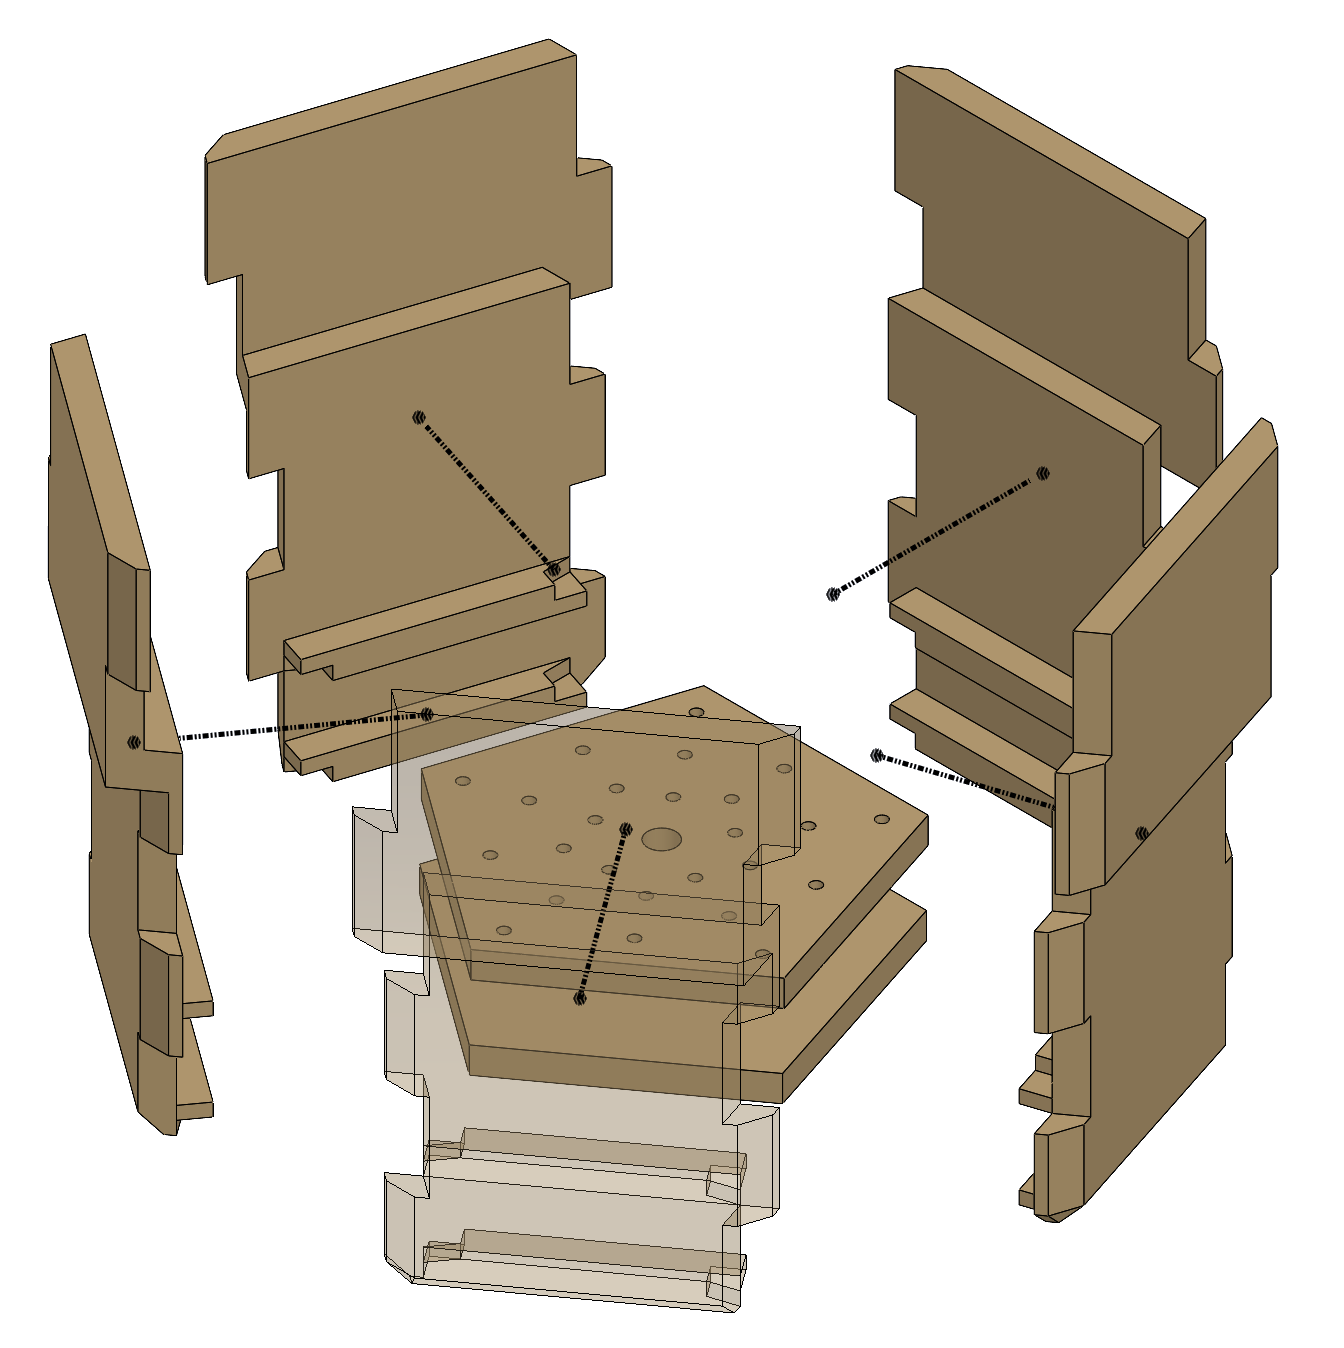
\includegraphics[scale=0.3]{images/screenshots/exploded_view_pent_pot.png}
    \caption{The above graphic contains an explosion diagram of all the parts assembling into a pentagonal pot.}
    \label{fig:pent_pot_explosion_diagram}
\end{figure}
After the three individual components for the plant pots are manufactured and coated with the biopolymer seal separately for both the pentagonal and the hexagonal pot, they can easily be assembled as shown in figure \ref{fig:pent_pot_explosion_diagram} with the help of wood glue to increase structural integrity and prevent leaks along the edges. Before assembly, a wick of approximately 5 cm needs to be installed in the inner bottom part.

\textit{The detailed explosion diagrams for both types of pots are present in Appendix Section \ref{technical_drawing:entire_exploding_technical_drawing}.}

\pagebreak
\subsubsection{Entire Structure}
\begin{figure}[H]
    \centering
    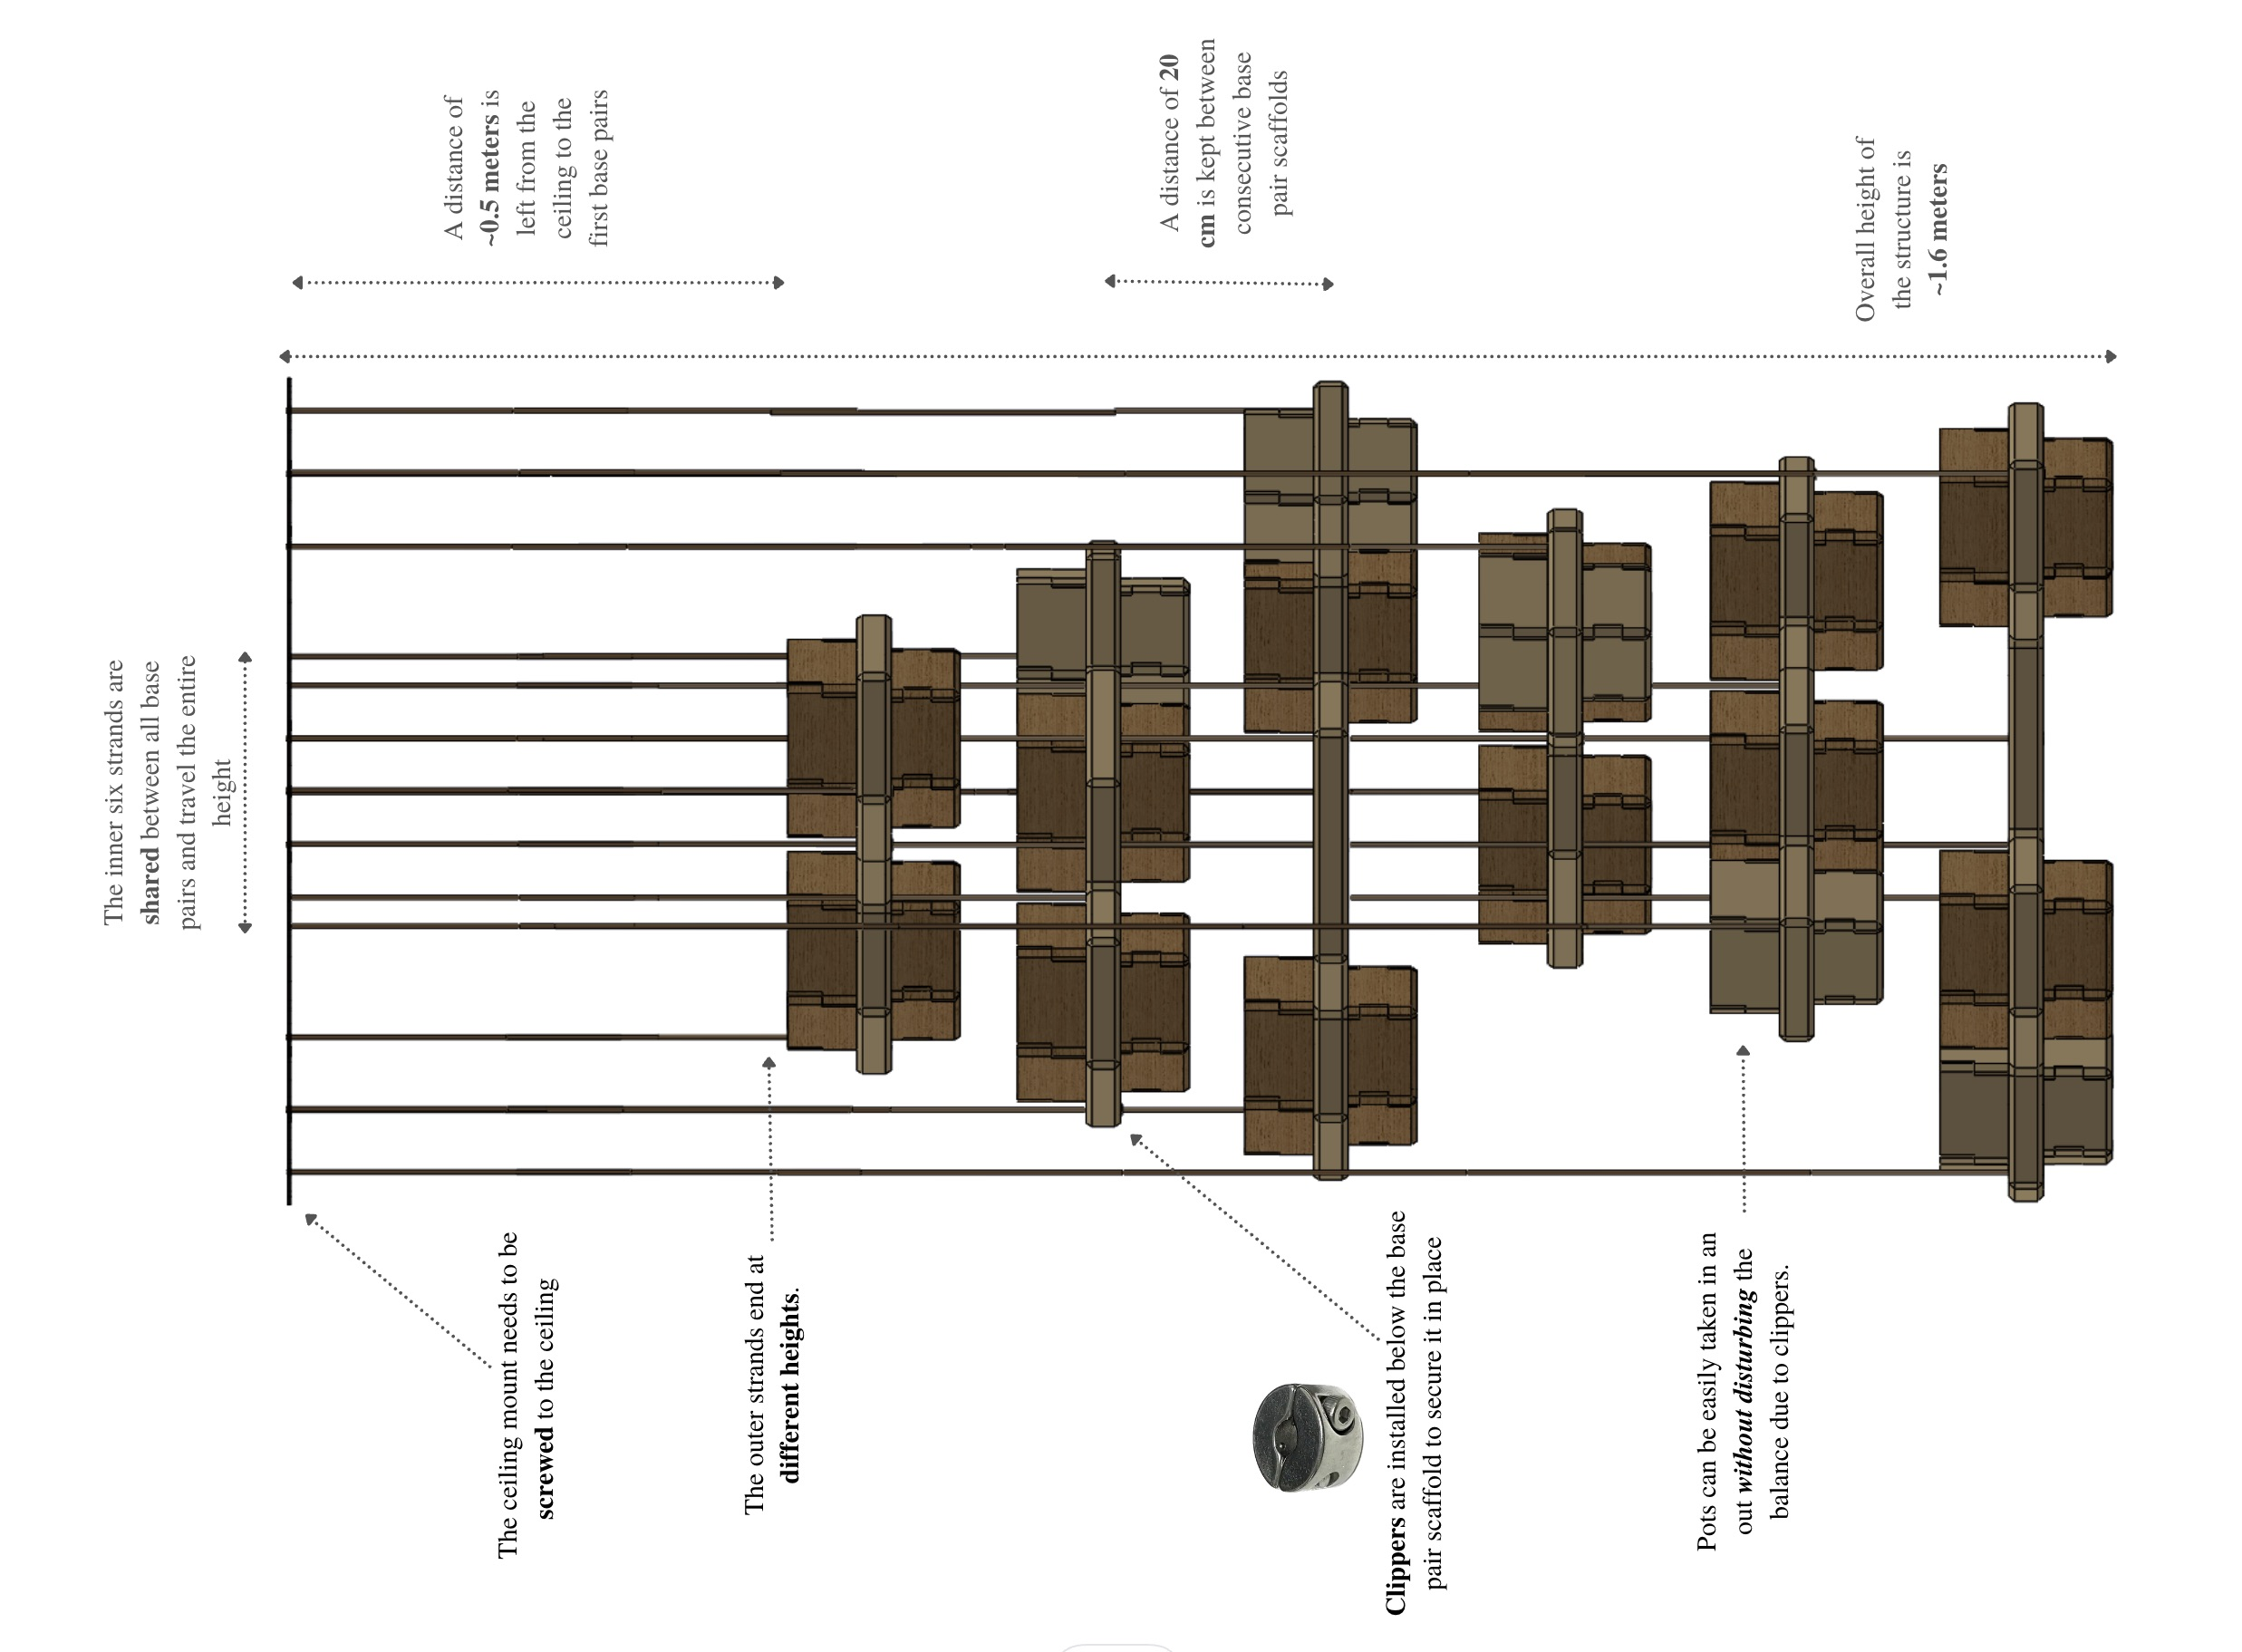
\includegraphics[scale=0.24, angle=-90]{images/screenshots/assembly_instructions.jpeg}
    \caption{The above graphic contains instructions to assemble the entire structure.}
    \label{fig:entire_assembly_instructions}
\end{figure}

After the individual plant pots have been assembled and the base-pair scaffolding manufactured, the final step is to assemble the entire structure as per the annotated graphic above.  
\pagebreak
\subsection{Fulfilment of the criteria}
\begin{itemize}
    \item \textbf{Design}: Our proposed ensemble takes heavy inspiration from Bioengineering by encapsulating the double-helical structure of DNA. We carefully decided the number of base pair scaffolds and angle of rotation in such a way as to ensure that the helix is easily observable.
    \item \textbf{Suitability to House Edible Plants}: We designed the pots to allow for the cultivation of edible plants. The dimensions of our
pots (10 cm in diameter, and 12.5 cm in depth) allow cultivation of various compact edible plants, such as herbs (e.g. Mint or Basil), Purslane, or microgreens. In the larger, hexagonal pots, even small varieties of \textbf{strawberries}, such as Mignonette, Alexandria, or
Fresca can also be grown. In the end, the specific species and variety of fruit that can be cultivated in the pots depend largely on variables independent of the design, such as individual preference and the amount of sunlight available in the room.
\item \textbf{Suitability for Office Spaces}: Our deliberate choice of suspending the entire structure from the ceiling makes it easy to install this ensemble in any office space by reducing its footprint. Moreover, we chose edible plants that can grow even with hindered sunlight and watering. If chosen to be hung in a more public area inside the Department of Bioengineering, the structure could also serve a secondary purpose as art to add to the aesthetics of a space. This makes our design an ideal choice for office spaces in the Bioengineering Department, the Student Common Room, or any other space on Imperial's campus.
\item \textbf{Sustainability}: Our choice of materials speaks for sustainability itself. We rigorously screened through our design choices to only select the most sustainable, and natural materials in our design (explained in depth in section \ref{topic:choice_of_materials}. Our design has \textbf{\textit{zero plastic usage}} and is almost \textbf{\textit{entirely biodegradable}}. 
\item \textbf{Cost}: Keeping the overall cost manageable was one of our primary constraints. As apparent from the Bill of Materials (section \ref{topic:bill_of_materials}), the overall material cost of the entire ensemble is 78 GBP which is a rather reasonable price for such installation. 
\item \textbf{Overall Quality}: Our choice of using wood as the primary material ensured a high-quality feel to the overall structure as opposed to using plastic. Wood renders a more natural and organic aesthetic.  Moreover, the choice of Tung Oil over varnish or beeswax also allowed the added benefit of providing a rich glossy finish to the wood. 
\item \textbf{Ease of Assembly}: Four manufacturing techniques were proposed in our design: CNC milling, Laser cutting, Metal cutting, and Metal drilling. These are very common techniques that would be available at Imperial facilities. The rest of the assembly can be carried out manually without any specialised equipment.
\end{itemize}

\pagebreak
\section{Reflective statement}
The insights we gained from our previous experiences with the DAPP portfolio played a vital role in the design process of our Bioengineering-inspired plant pot. We began by engaging in lively discussions and brainstorming sessions, drawing on our design expertise. The importance of our sketching skills became evident as we utilised digital notebooks to transform our ideas into tangible designs. Our proficiency in sketching greatly enhanced our ability to articulate intricate design choices. 
 
Transitioning from rough on-paper sketches to a more immersive 3D representation, we leveraged our CAD skills acquired through SolidWorks lessons. This allowed us to create high-fidelity models with precise specifications, encompassing material types, weights, joints, edges, and more. The ability to accurately define these details facilitated a clearer manufacturing outline for our design.

Finally, Blender was used to take our SolidWorks models and bring them to life with the addition of the wood stains we wanted to use and with plants to get a better feel for what our design would look like in an environment. This also helps show an audience what to expect from the completed pot assembly.
 
Drawing on our knowledge from the Materials and Common Manufacturing Techniques lesson, we ensured that our manufacturing plans were well-informed. We carefully considered material choices and their impact on the overall design, taking into account factors such as durability, sustainability, and cost-effectiveness. We paired our learning on material properties and failure from "Fundamentals of Biomedical Engineering" with SolidWorks's static simulation analysis in order to assure the structural integrity of our design.

Furthermore, our experience working collaboratively as a team on the Ethics report proved invaluable in organising and distributing tasks effectively. We recognised the importance of leveraging each team member's strengths and ensuring that everyone's perspectives were heard and considered. This collaborative approach allowed us to strike a balance between open discussions and making decisive design choices, propelling us forward as a cohesive unit. 
 
Overall, our prior knowledge and experiences in the DAPP portfolio served as the foundation for our success in designing the Bioengineering-inspired plant pot. By incorporating our sketching skills, CAD proficiency, Blender, knowledge of materials and manufacturing techniques, and effective teamwork, we were able to create a design that seamlessly merged creativity, functionality, and practicality. 
\section{References}
\printbibliography[heading=none]
\pagebreak
\section{Appendix}
For a better visual experience, we exported a short video from Blender highlighting the entire design. The video is located \href{https://drive.google.com/file/d/1XJ0yTDizML6BhURdkV9e93mYVJ_03wjc/view?usp=sharing}{here}.
We also exported all part files, assembly files, blender renders, and technical drawings located in this repository - \href{https://github.com/Sauciu1/DAPP-Plant-Pot-Design}{https://github.com/Sauciu1/DAPP-Plant-Pot-Design}. 

\subsection{Software/Tools Used}
We utilised \textbf{SolidWorks 2022} for the design and assembly of each component. We inferred additional material information using  \textbf{Ansys Grants EduPack}. For various figures mentioned in this report (see Figure \ref{fig:pent_pot}, Figure \ref{fig:hex_pot}, Figure \ref{fig:rendered_whole_structure}), we employed \textbf{Blender 3.5} shaders. For the annotations of various graphics (see Figure \ref{fig:ceiling_mount_annotated}, Figure \ref{fig:entire_assembly_instructions}), we used \textbf{Canva}. We used \textbf{Goodnotes} (iPad) and \textbf{Adobe Fresco} (iPad) for hand-drawn sketches. Finally, we used \textbf{ChatGPT} for grammar aid.

\subsection{Technical Drawings \& Additional Graphics}\label{topic:technical_drawings}

% Stress Test Image
\begin{figure}[!ht]
    \centering
    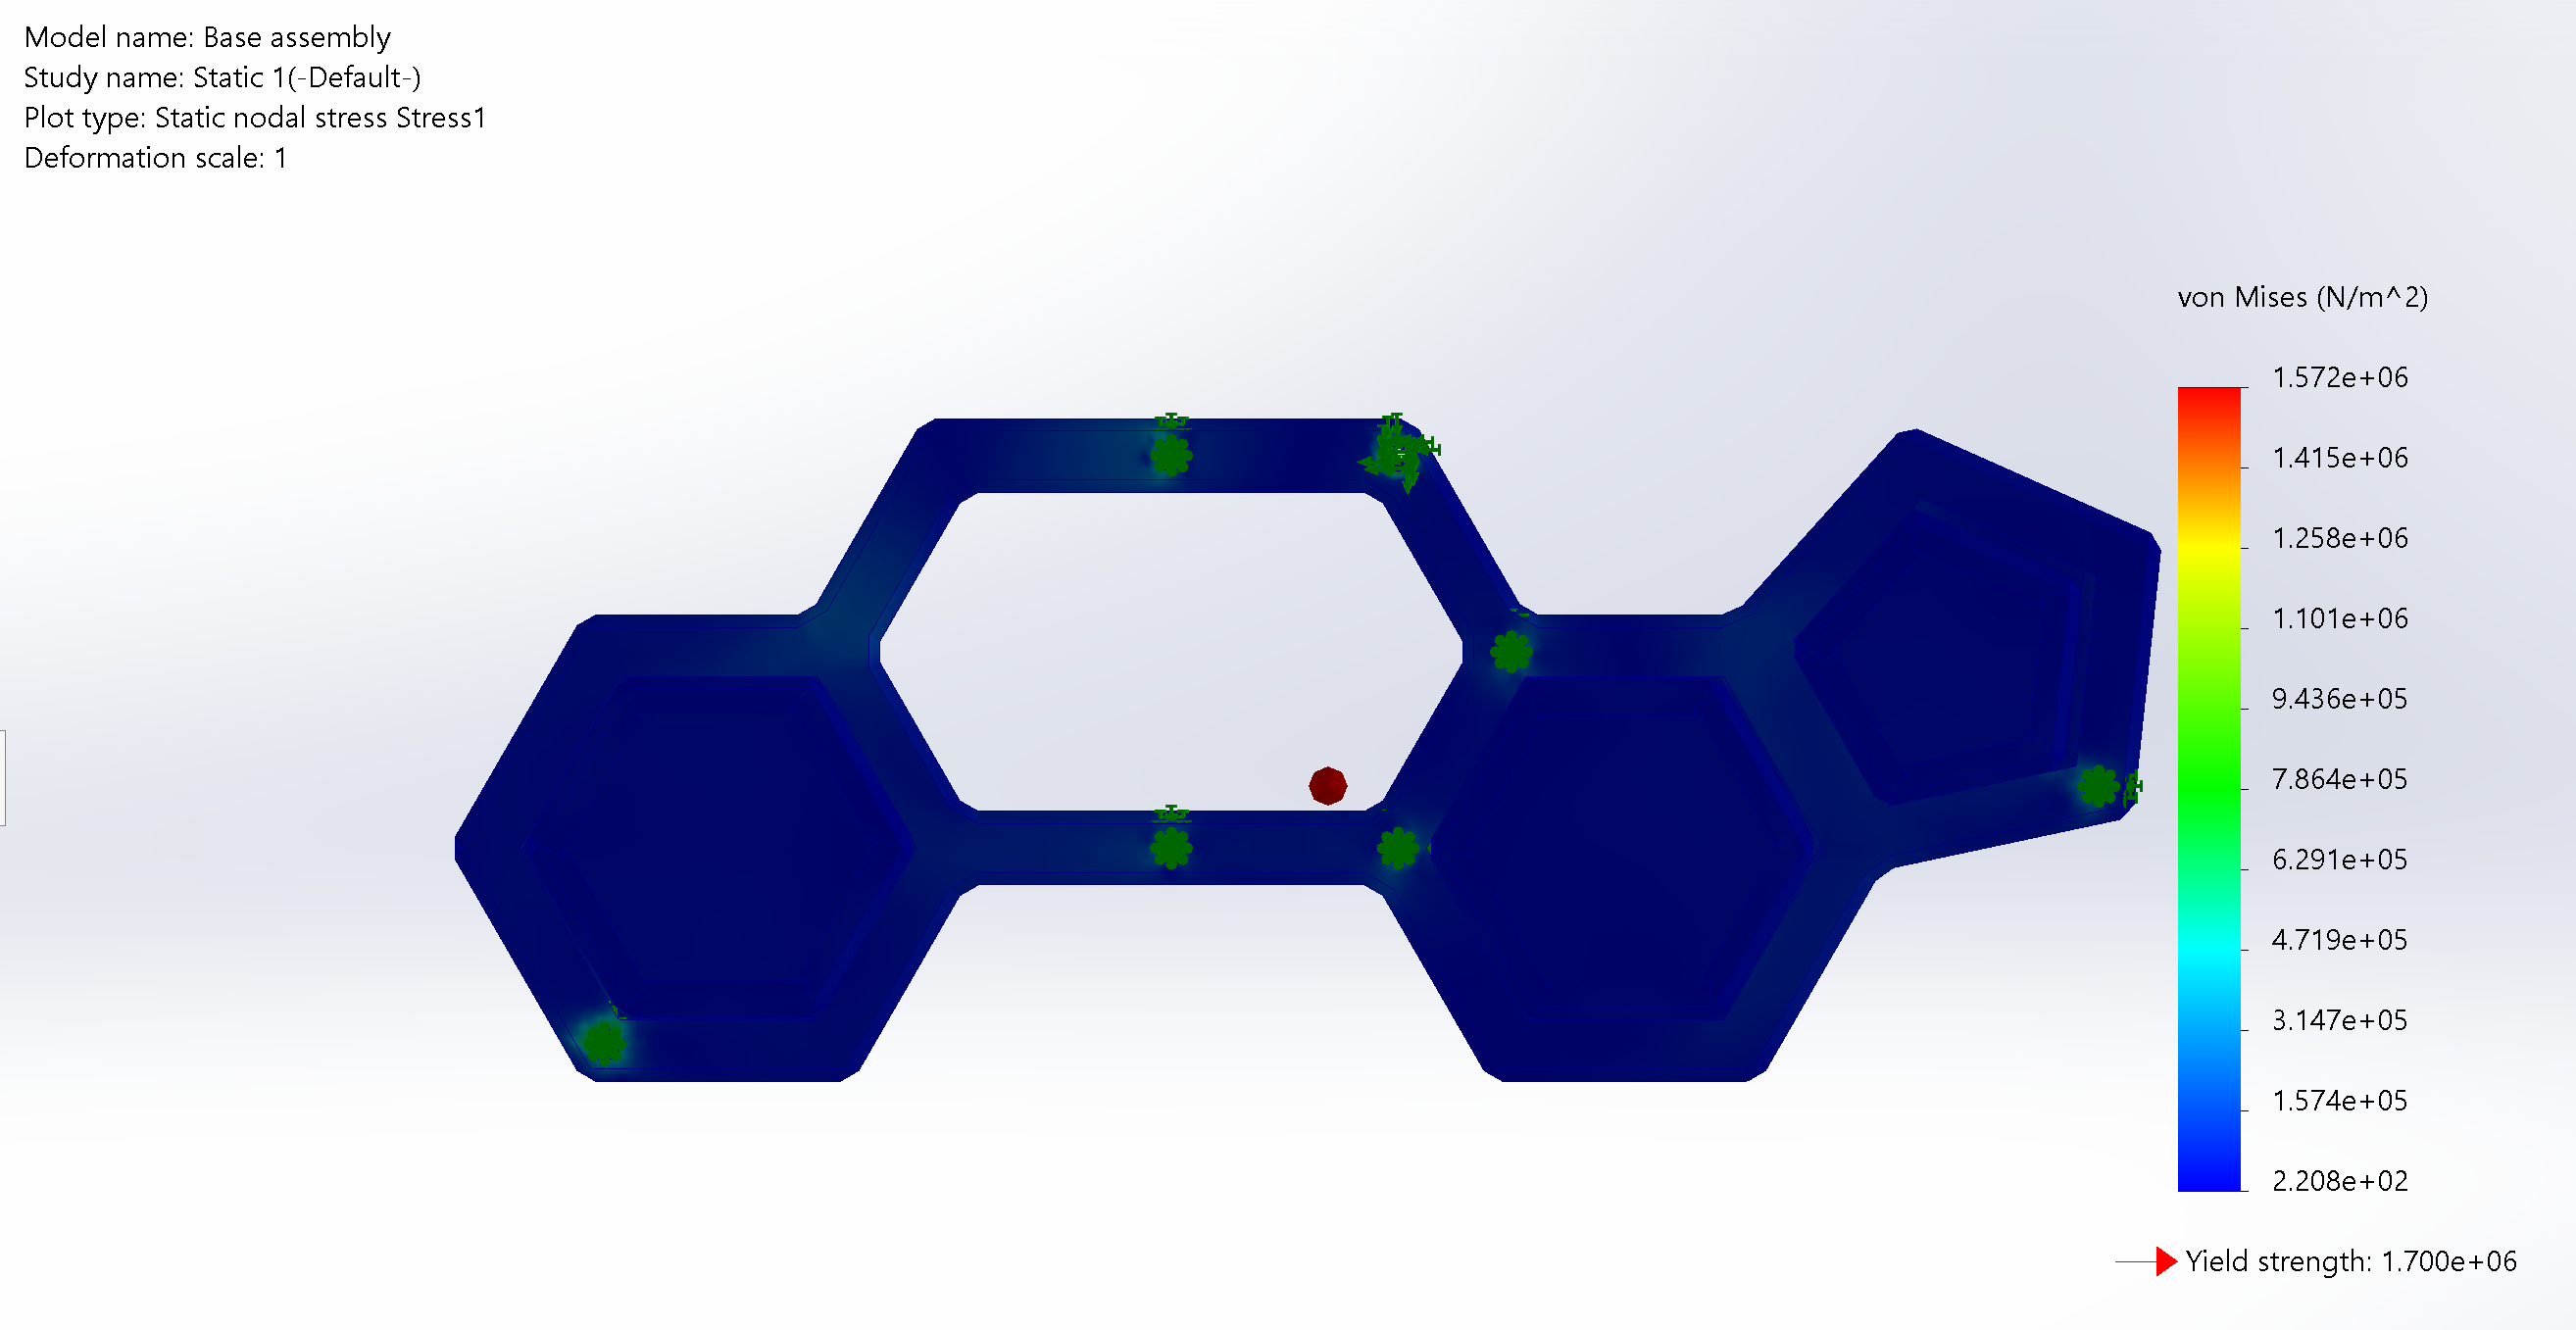
\includegraphics[width=1\textwidth]{images/screenshots/stress_test.png}
    \caption{A Screenshot is taken from SolidWorks denoting the points of maximum stress in the base pair structure. The green points serve as the string holes as explained in section \ref{para:max_stress}.}
    \label{screenshot:stress_test_image}
\end{figure}

% Base pair structure
\begin{sidewaysfigure}[!ht]
    \centering
    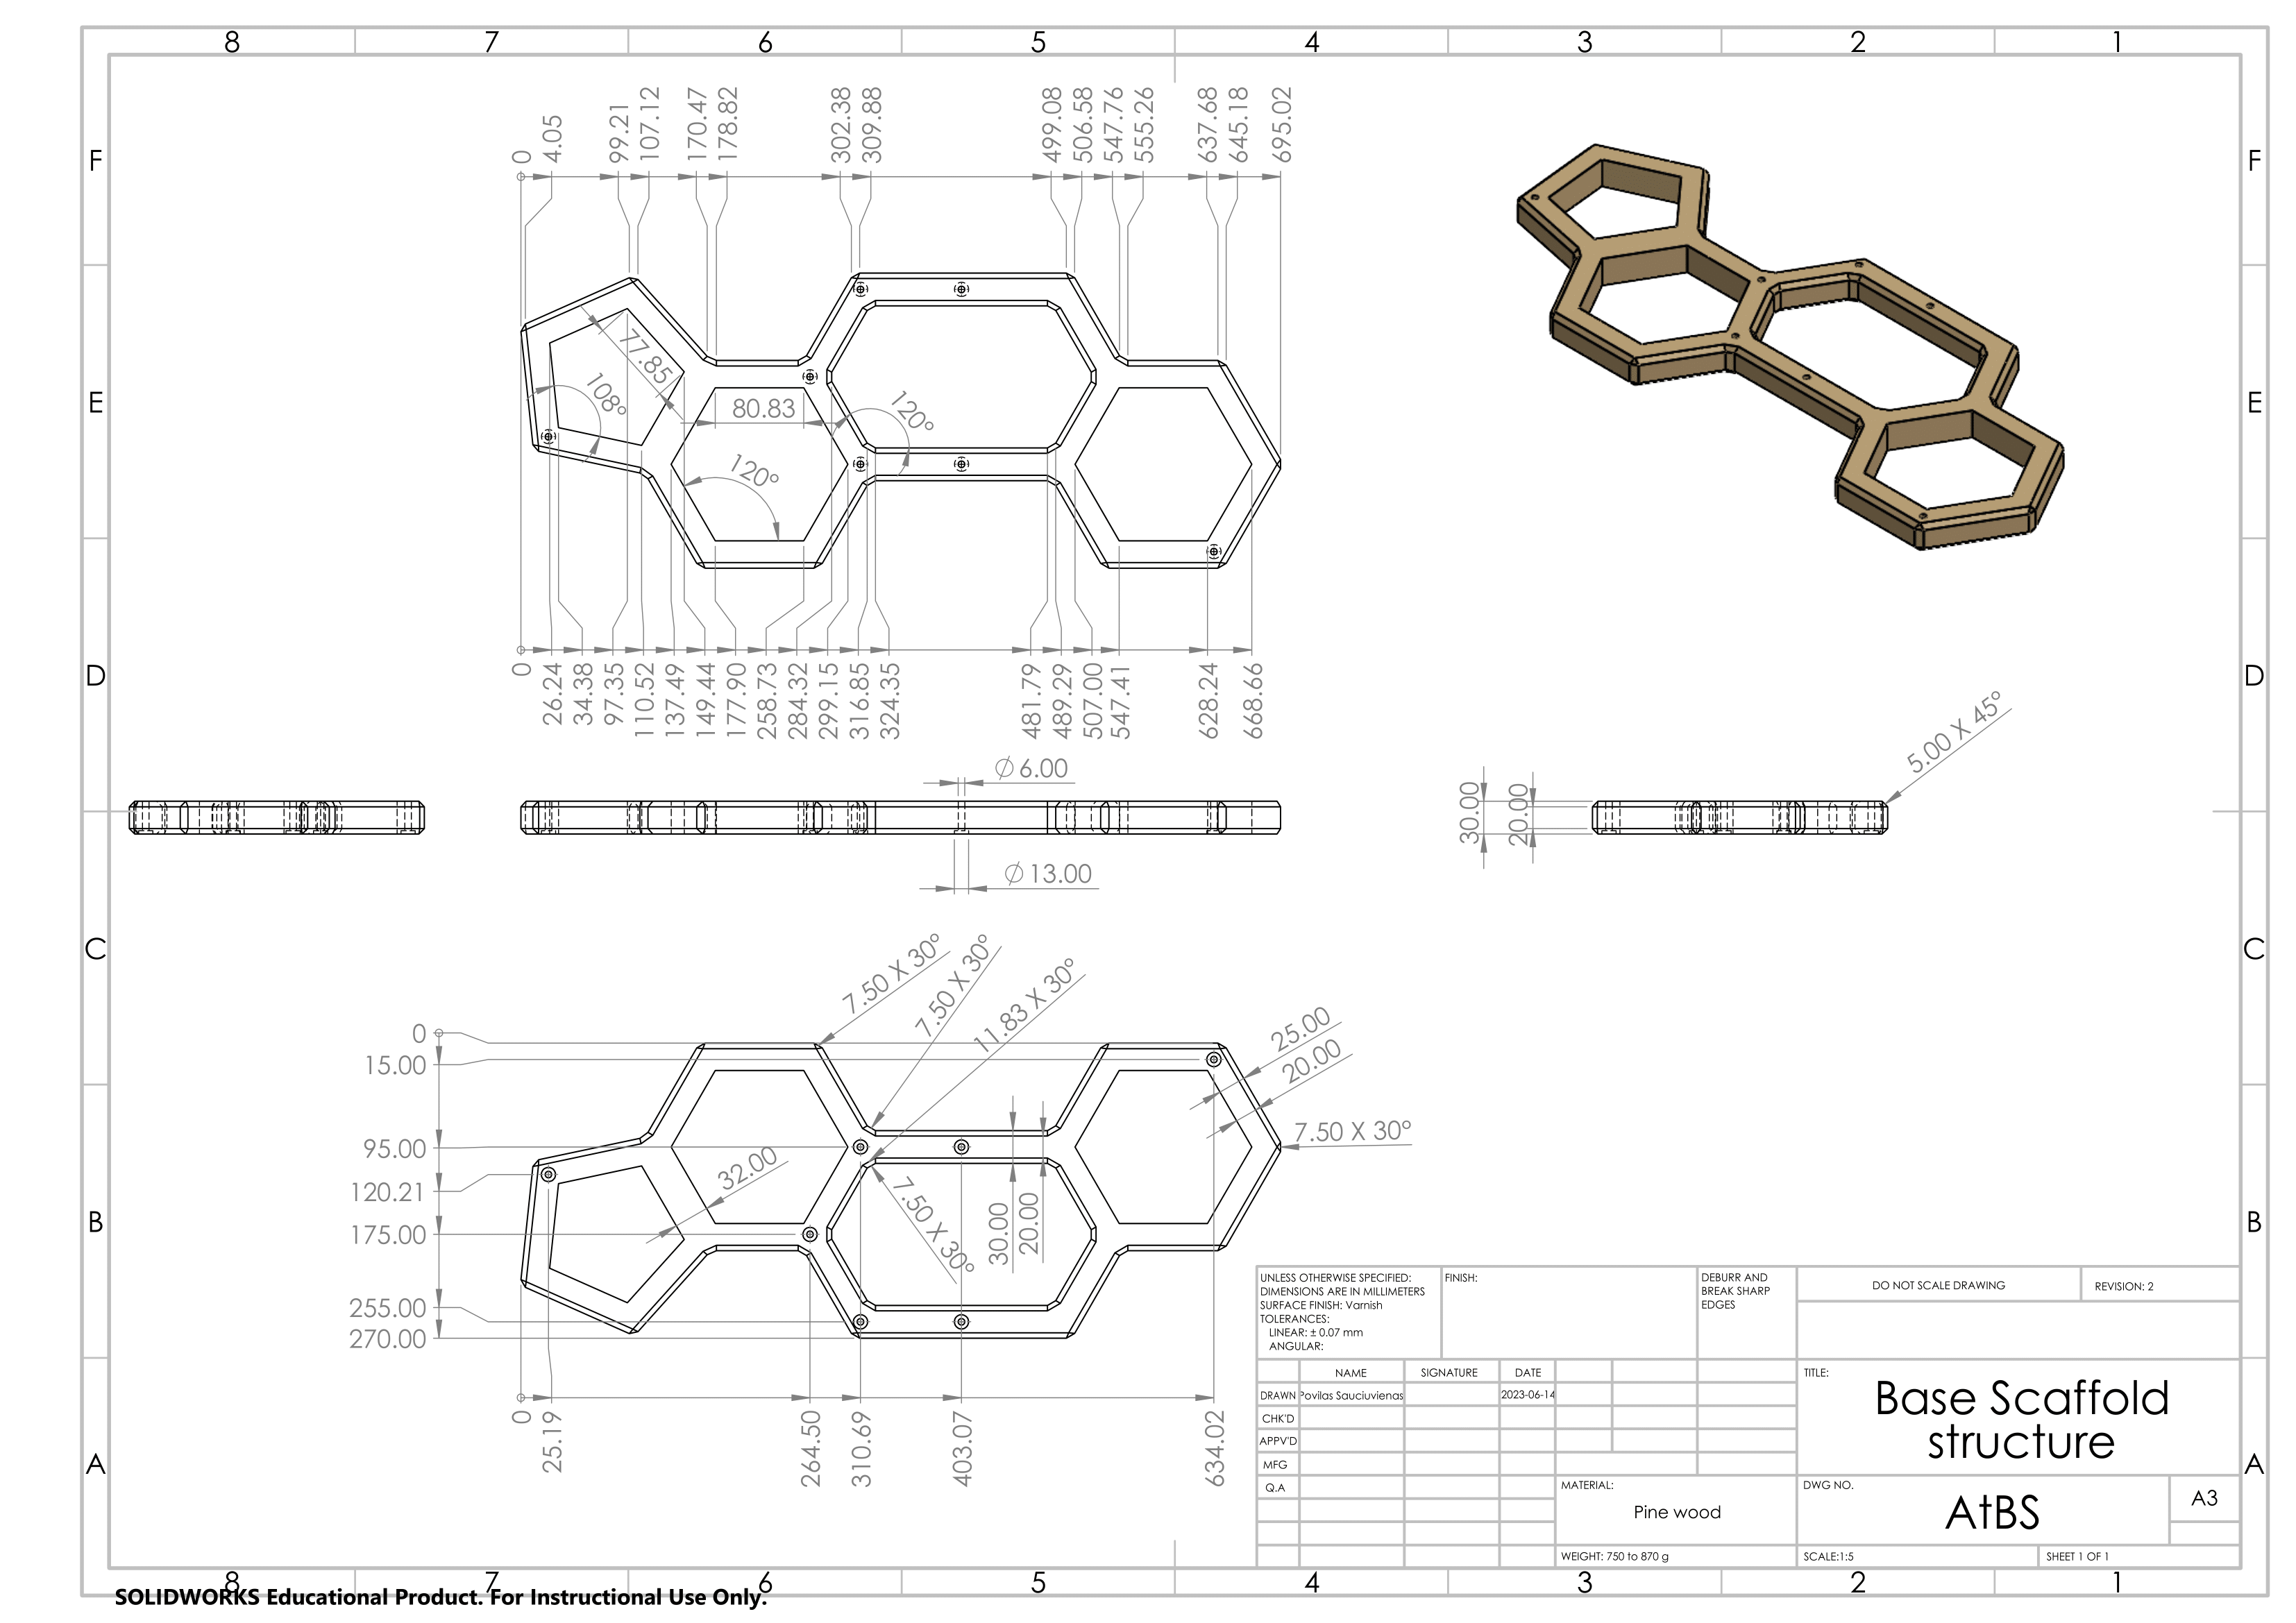
\includegraphics[width=1\textwidth ]{images/technical_drawings/Base structure-1.png}
    \caption{Technical drawing of the \textbf{base-pair structure} that is manufactured via CNC milling as explained in section \ref{topic:CNC_Milling}.}
    \label{technical_drawing:base_pair}
\end{sidewaysfigure}

% Ceiling Mount
\begin{sidewaysfigure}[!ht]
    \centering
    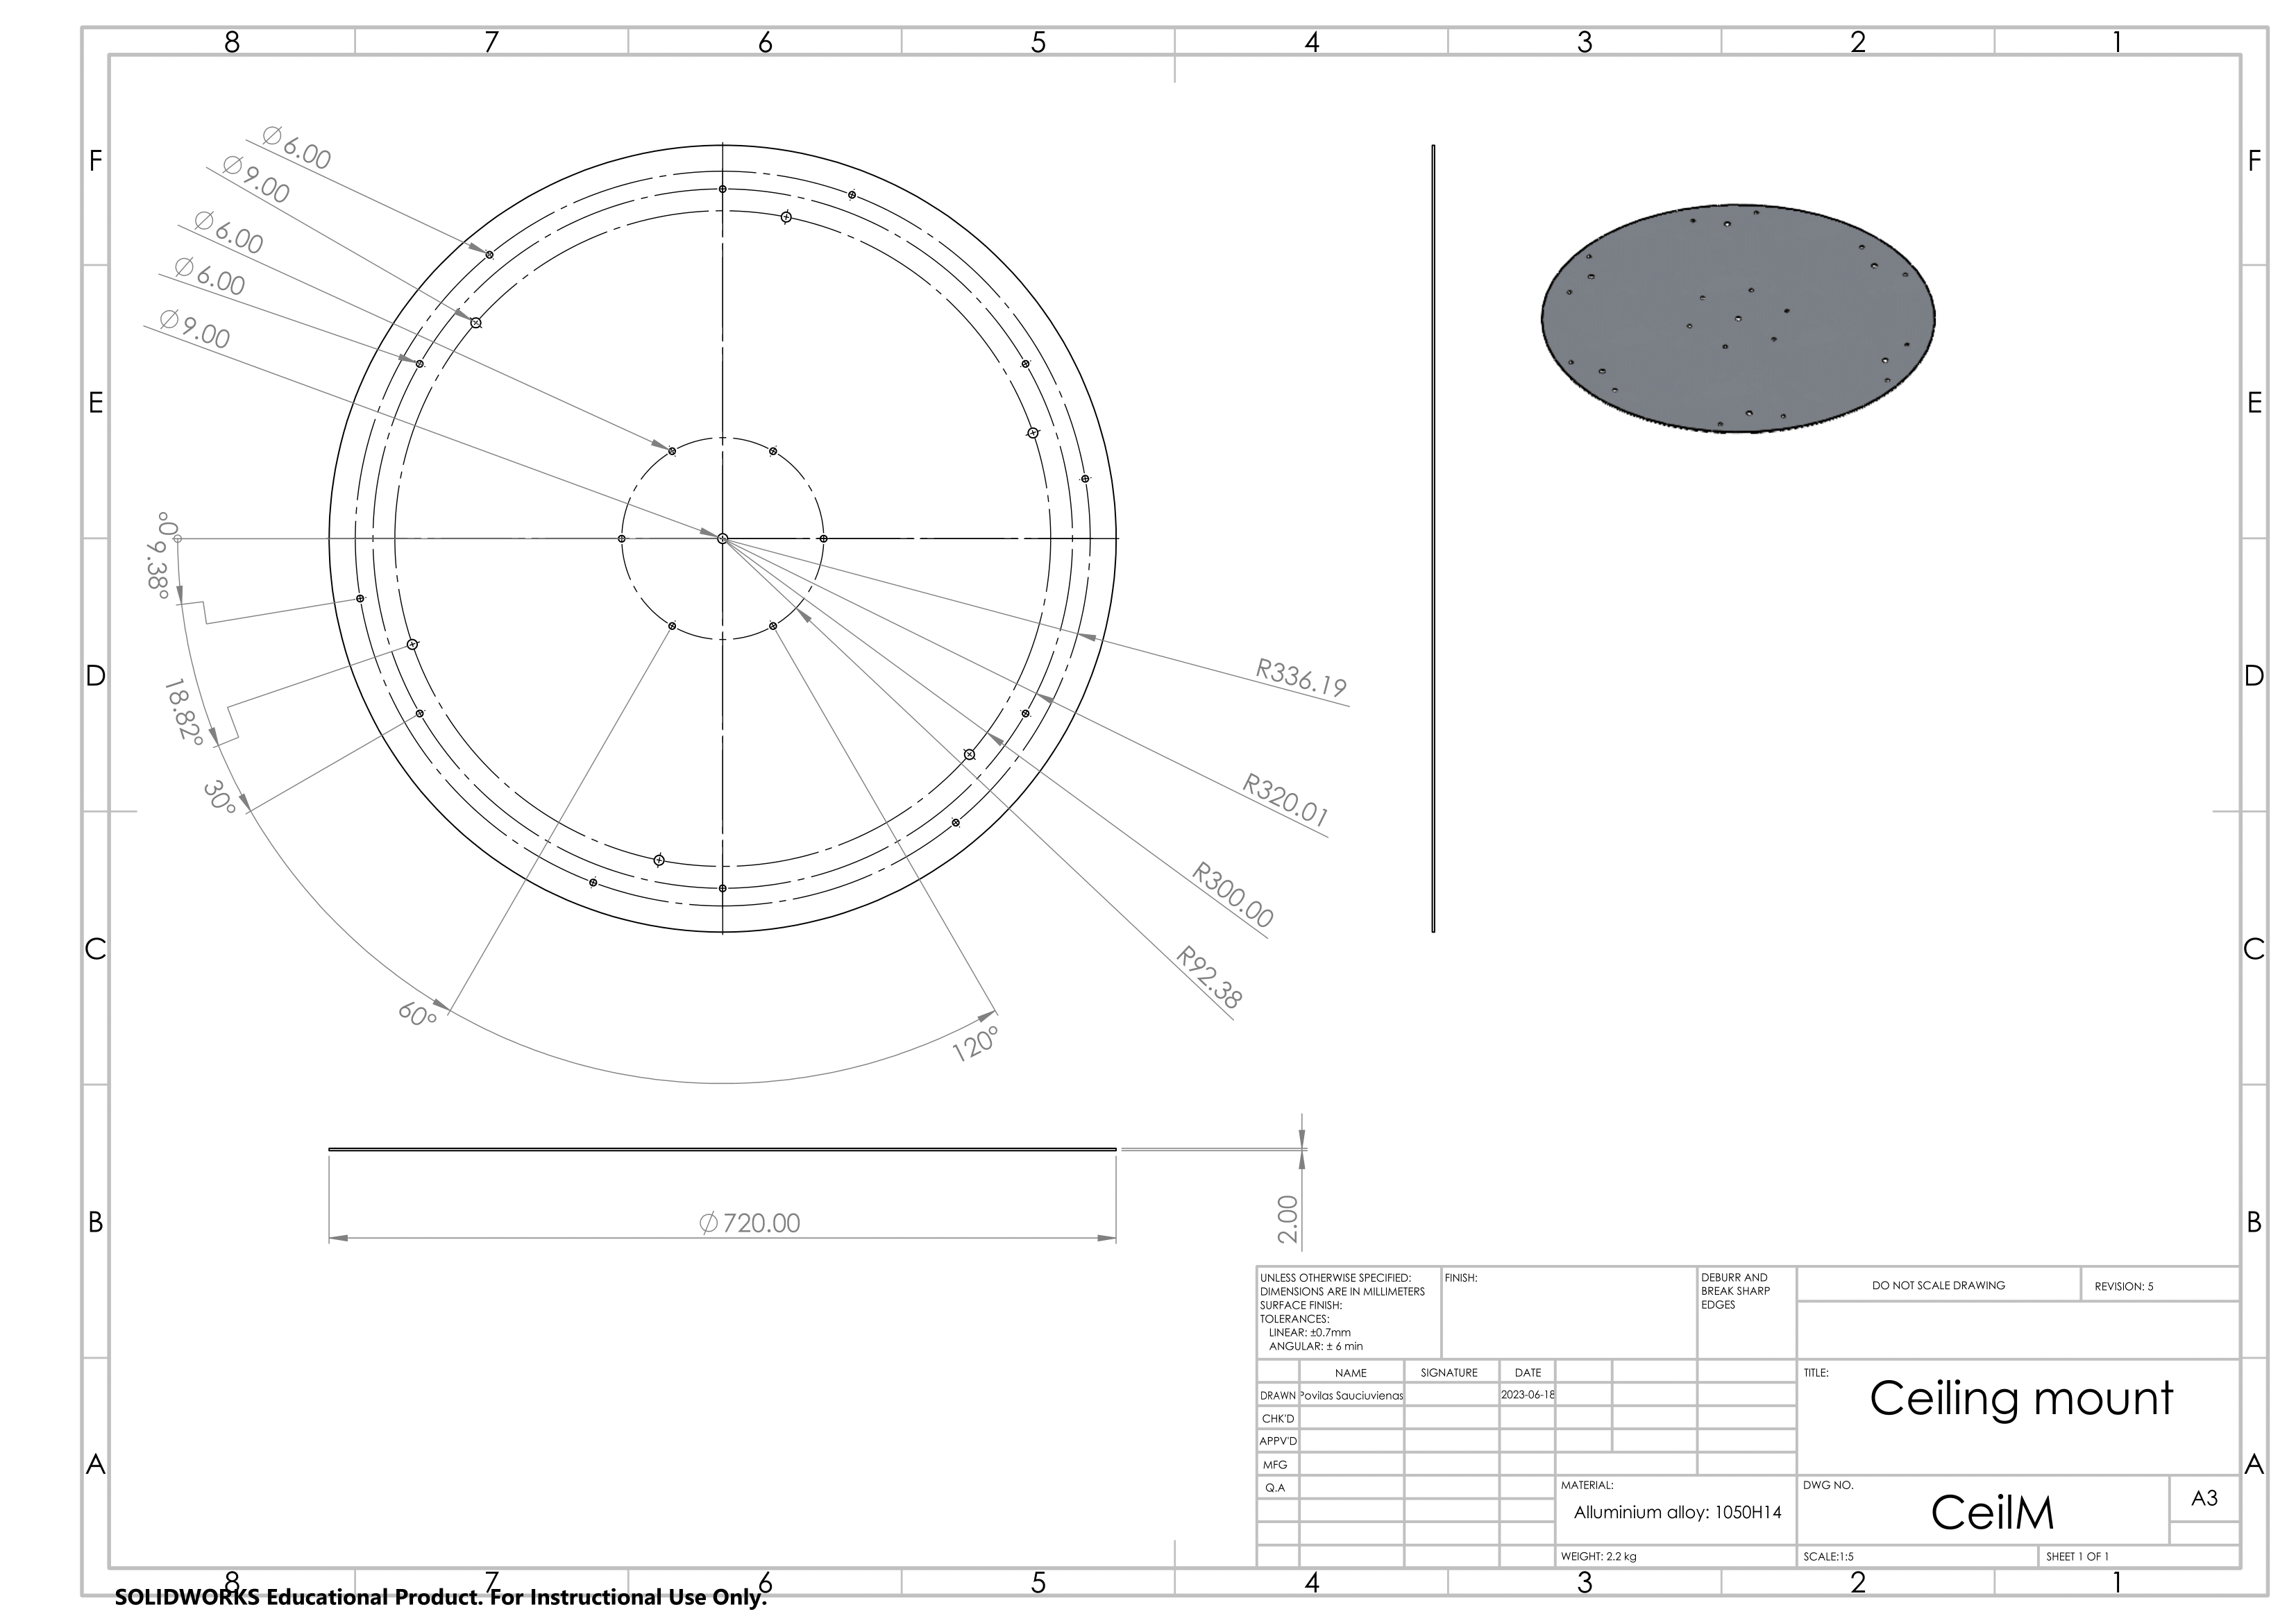
\includegraphics[width=1\textwidth ]{images/technical_drawings/Ceilling_mount_revised.png}
    \caption{Technical drawing of the \textbf{Ceiling Mount} used to suspend the ensemble from the ceiling. Explained in depth in section \ref{fig:ceiling_mount_annotated}.}
    \label{technical_drawing:ceiling_mount}
\end{sidewaysfigure}

% Entire Exploding View
\begin{figure}[ht]
    \centering
    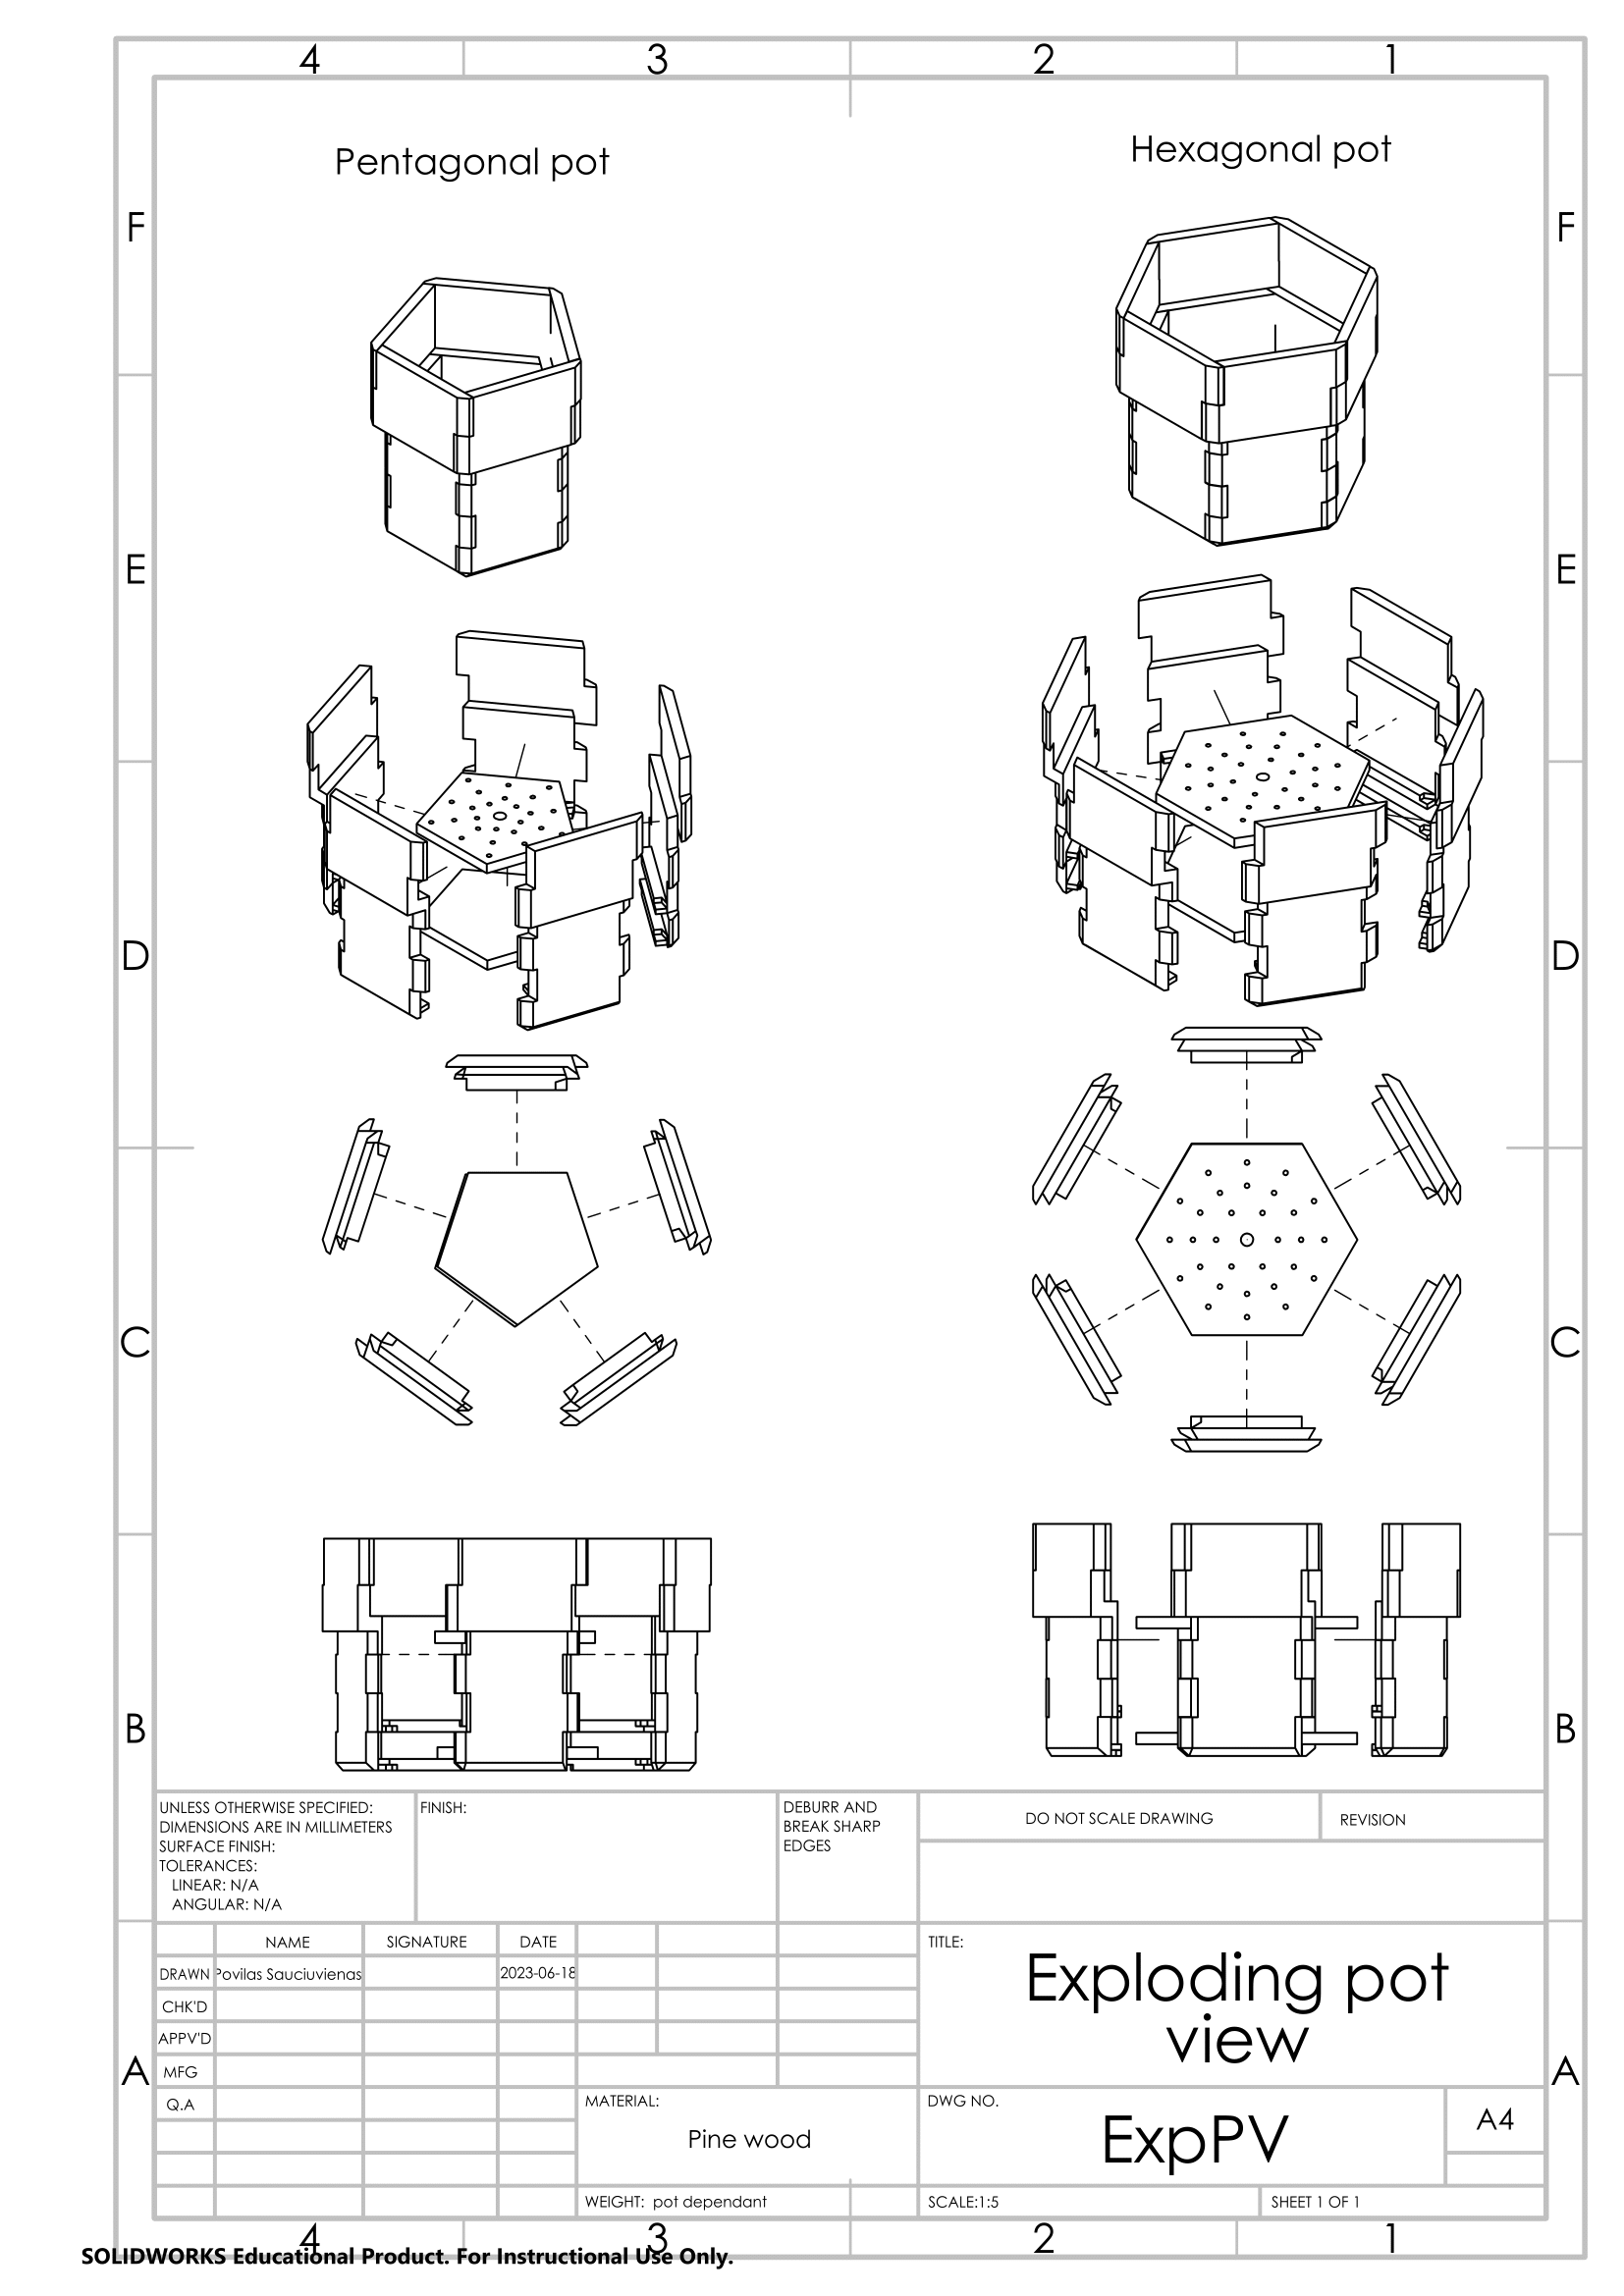
\includegraphics[width=0.9\textwidth]{images/technical_drawings/entire_exploding_technical_drawing.png}
    \caption{Technical drawing of the exploding view of both Pentagonal and Hexagonal Pots as described in the assembly section \ref{fig:pent_pot_explosion_diagram}.}
    \label{technical_drawing:entire_exploding_technical_drawing}
\end{figure}

% Hexagonal pot side part
\begin{sidewaysfigure}[!ht]
    \centering
    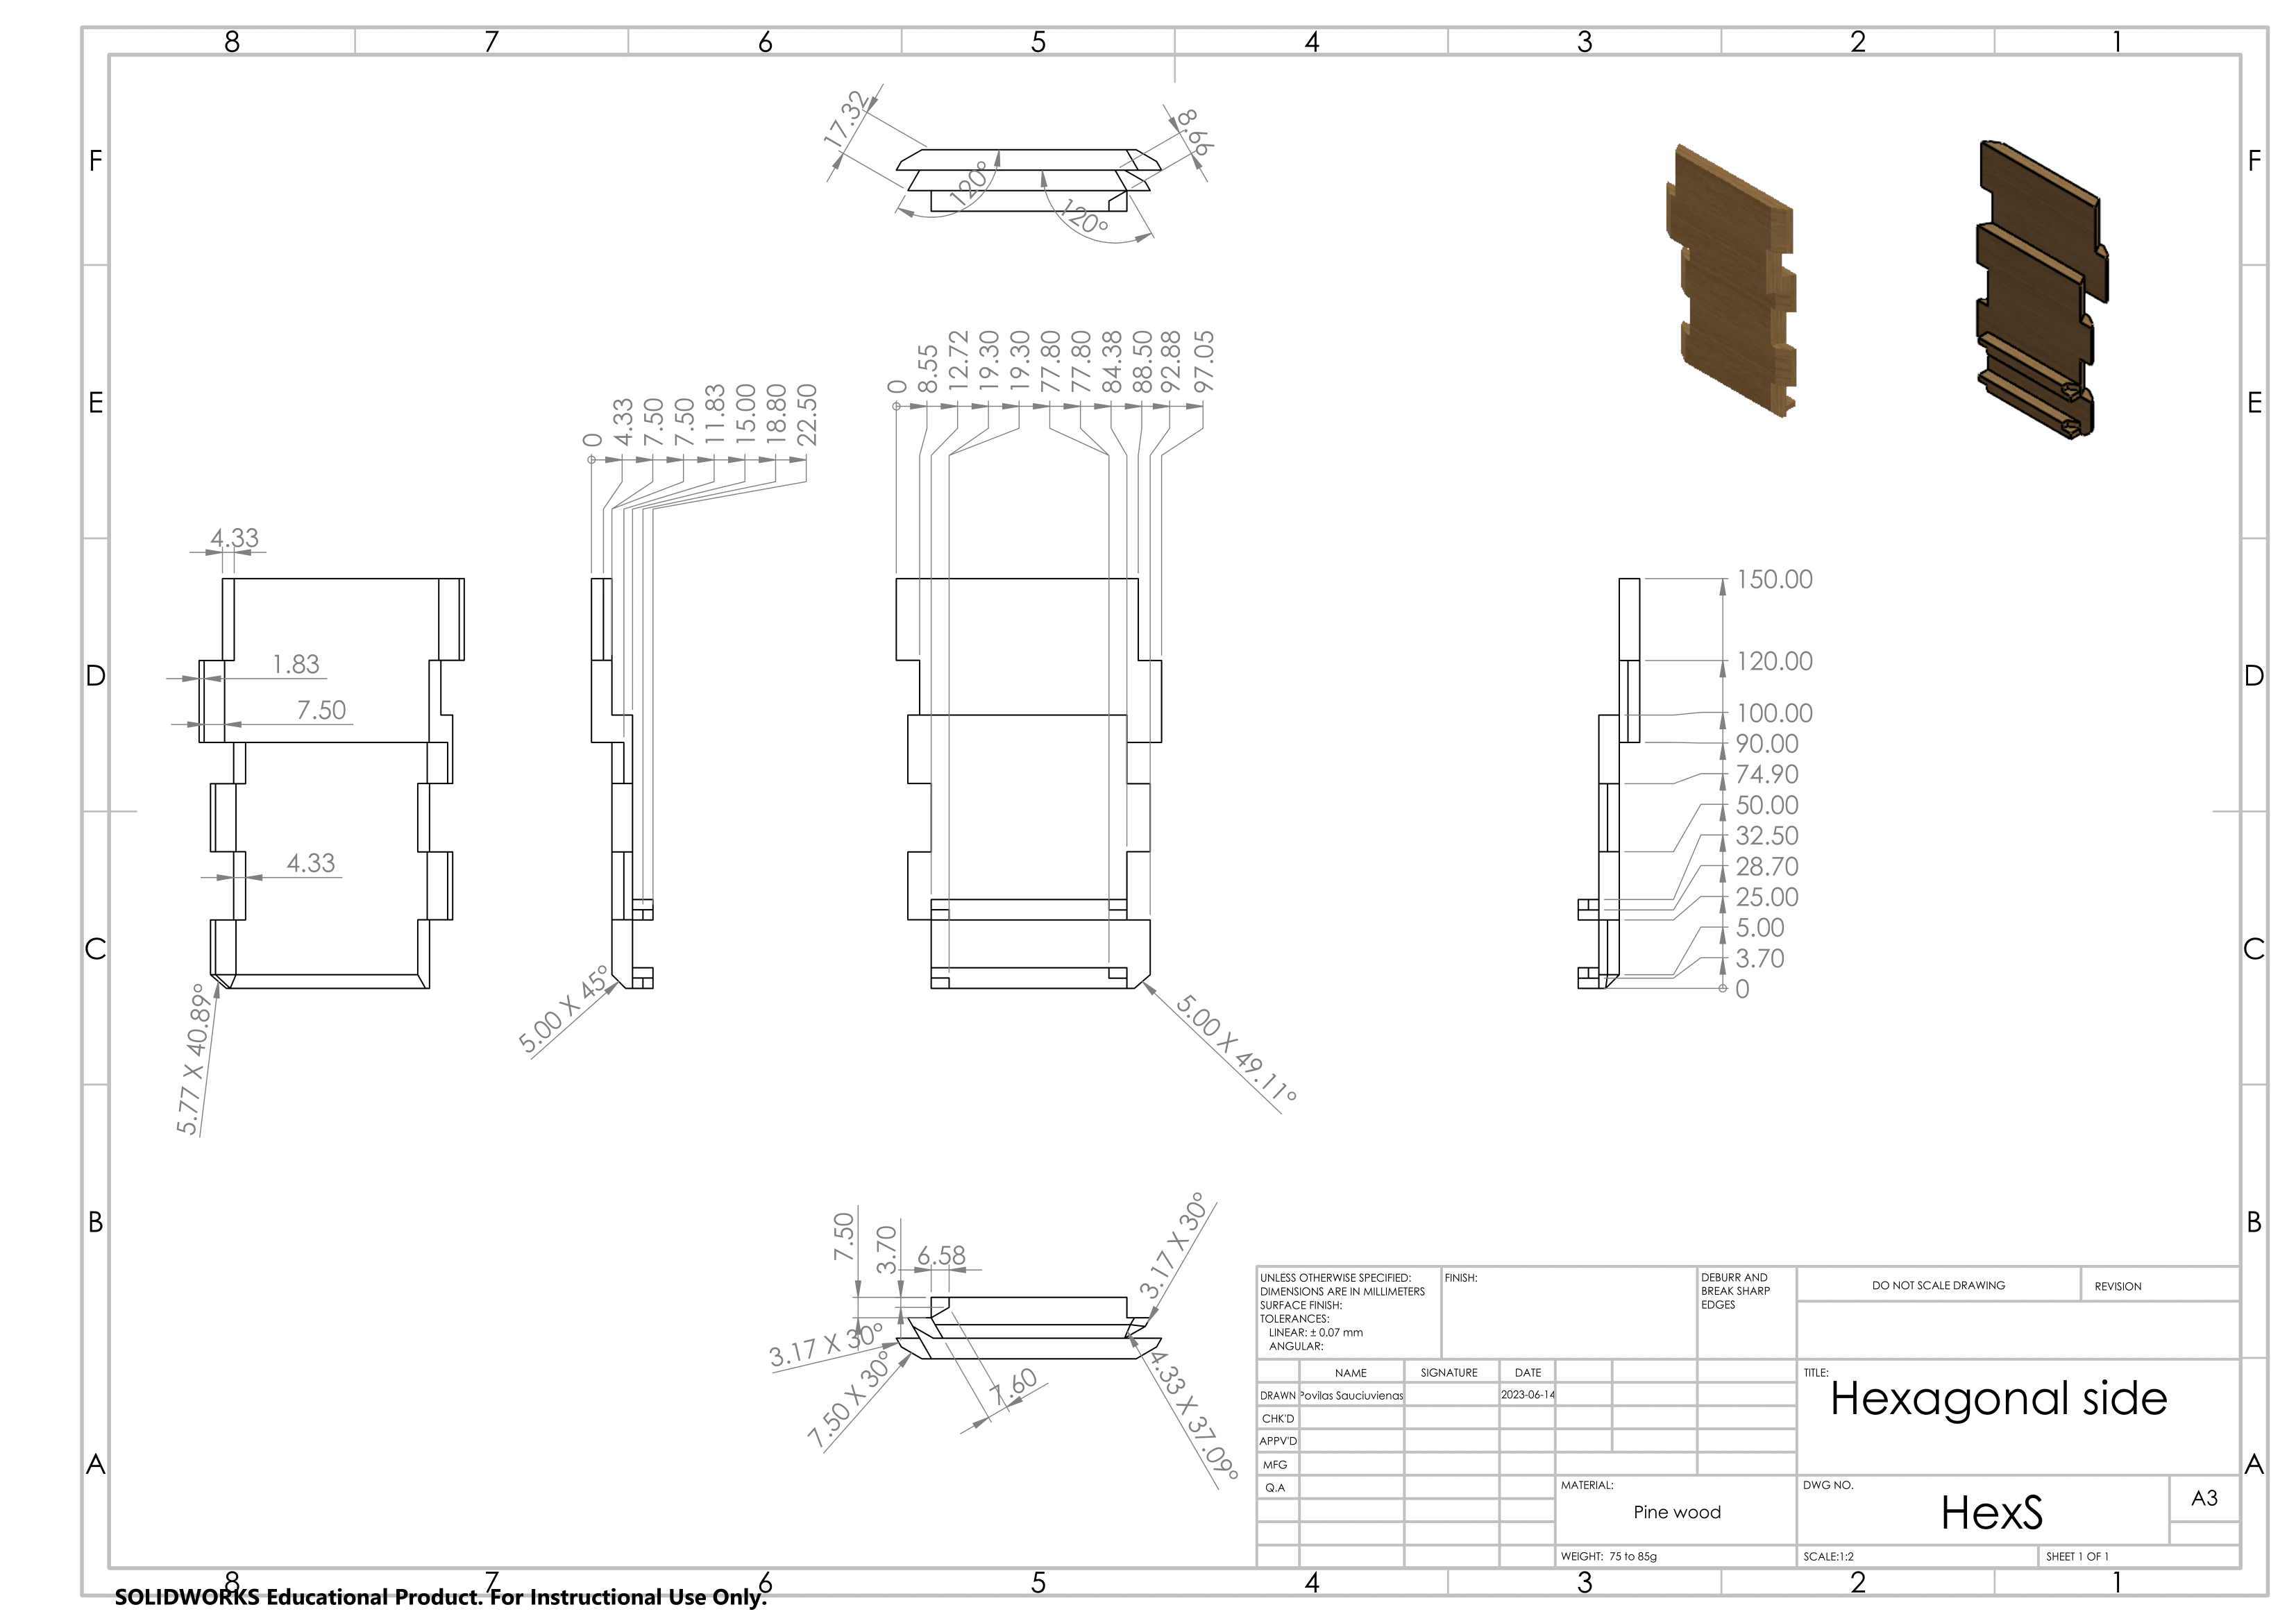
\includegraphics[width=1\textwidth ]{images/technical_drawings/Hexagonal side-1.png}
    \caption{Technical drawing of the \textbf{side part (one of six) of the hexagonal pot} required for assembly explained in section \ref{topic:CNC_Milling}.}
    \label{technical_drawing:hex_pot_side_part}
\end{sidewaysfigure}

% Hexagonal pot inner bottom
\begin{figure}[ht]
    \centering
    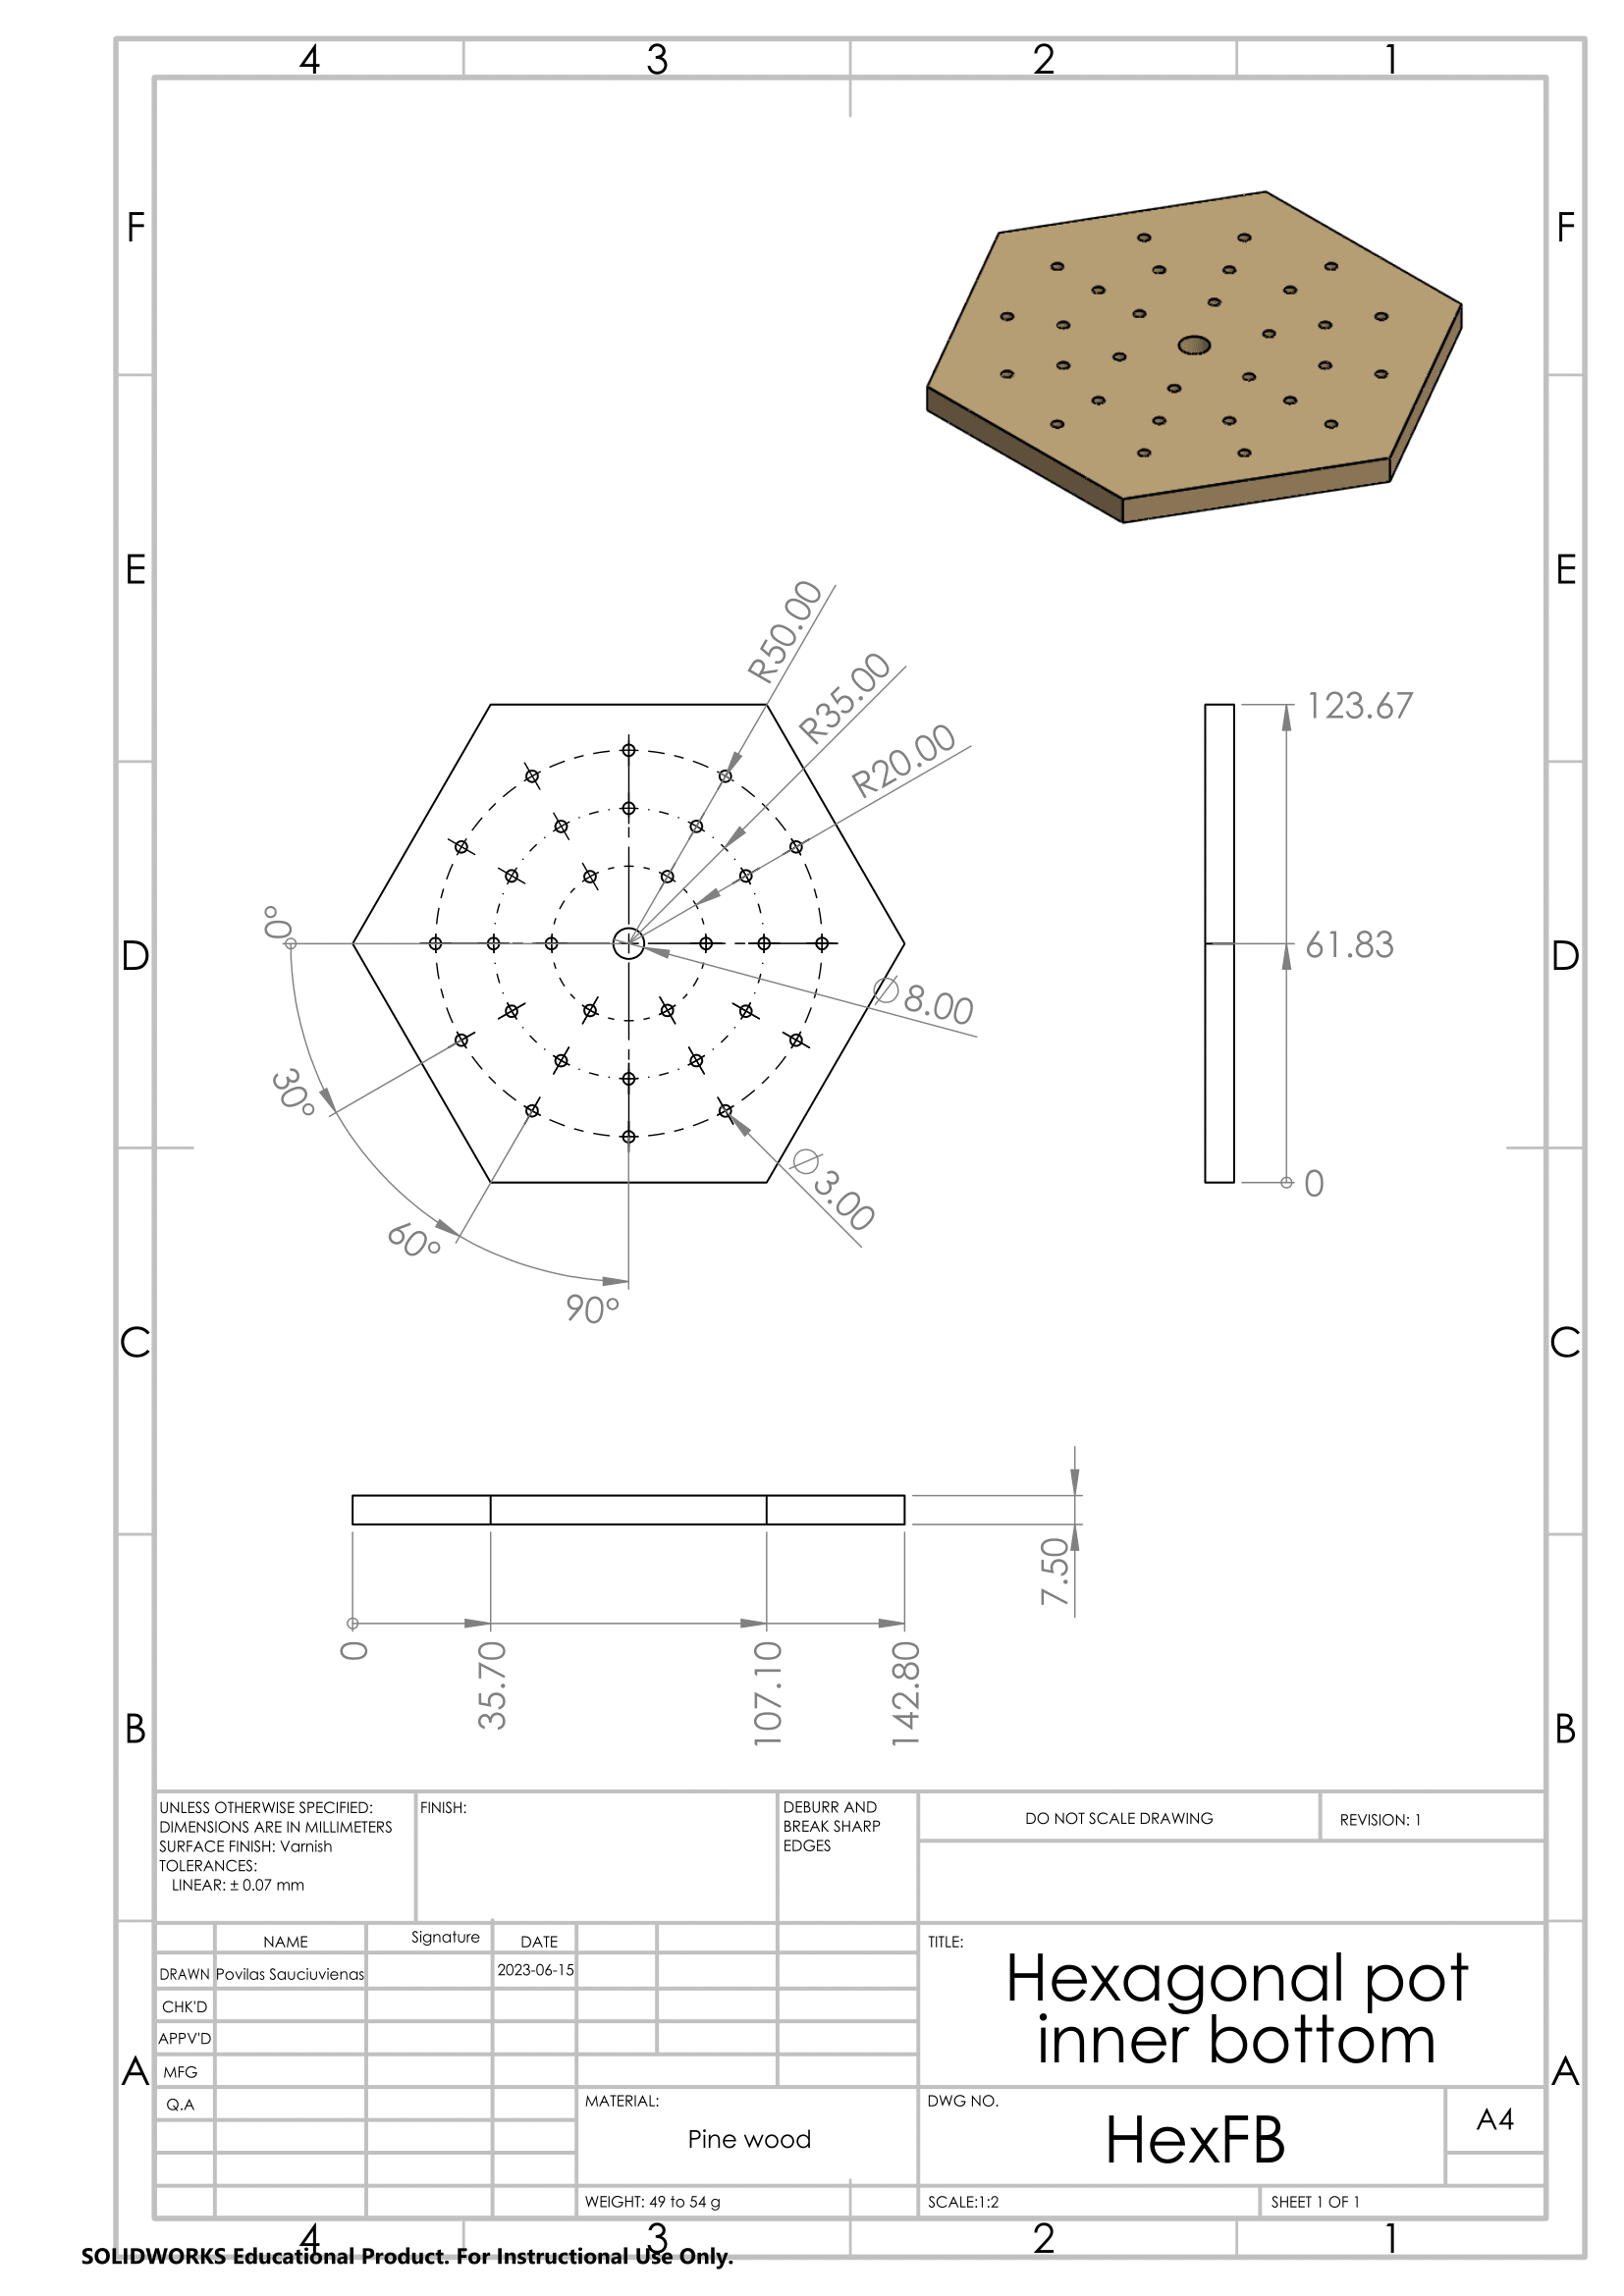
\includegraphics[width=0.9\textwidth]{images/technical_drawings/Hexagonal_pot_inner_bottom.png}
    \caption{Technical drawing of the \textbf{inner bottom of the hexagonal pot} required for assembly explained in section \ref{topic:CNC_Milling}.}
    \label{technical_drawing:hex_pot_inner_bottom}
\end{figure}

% Hexagonal pot outer bottom
\begin{figure}[ht]
    \centering
    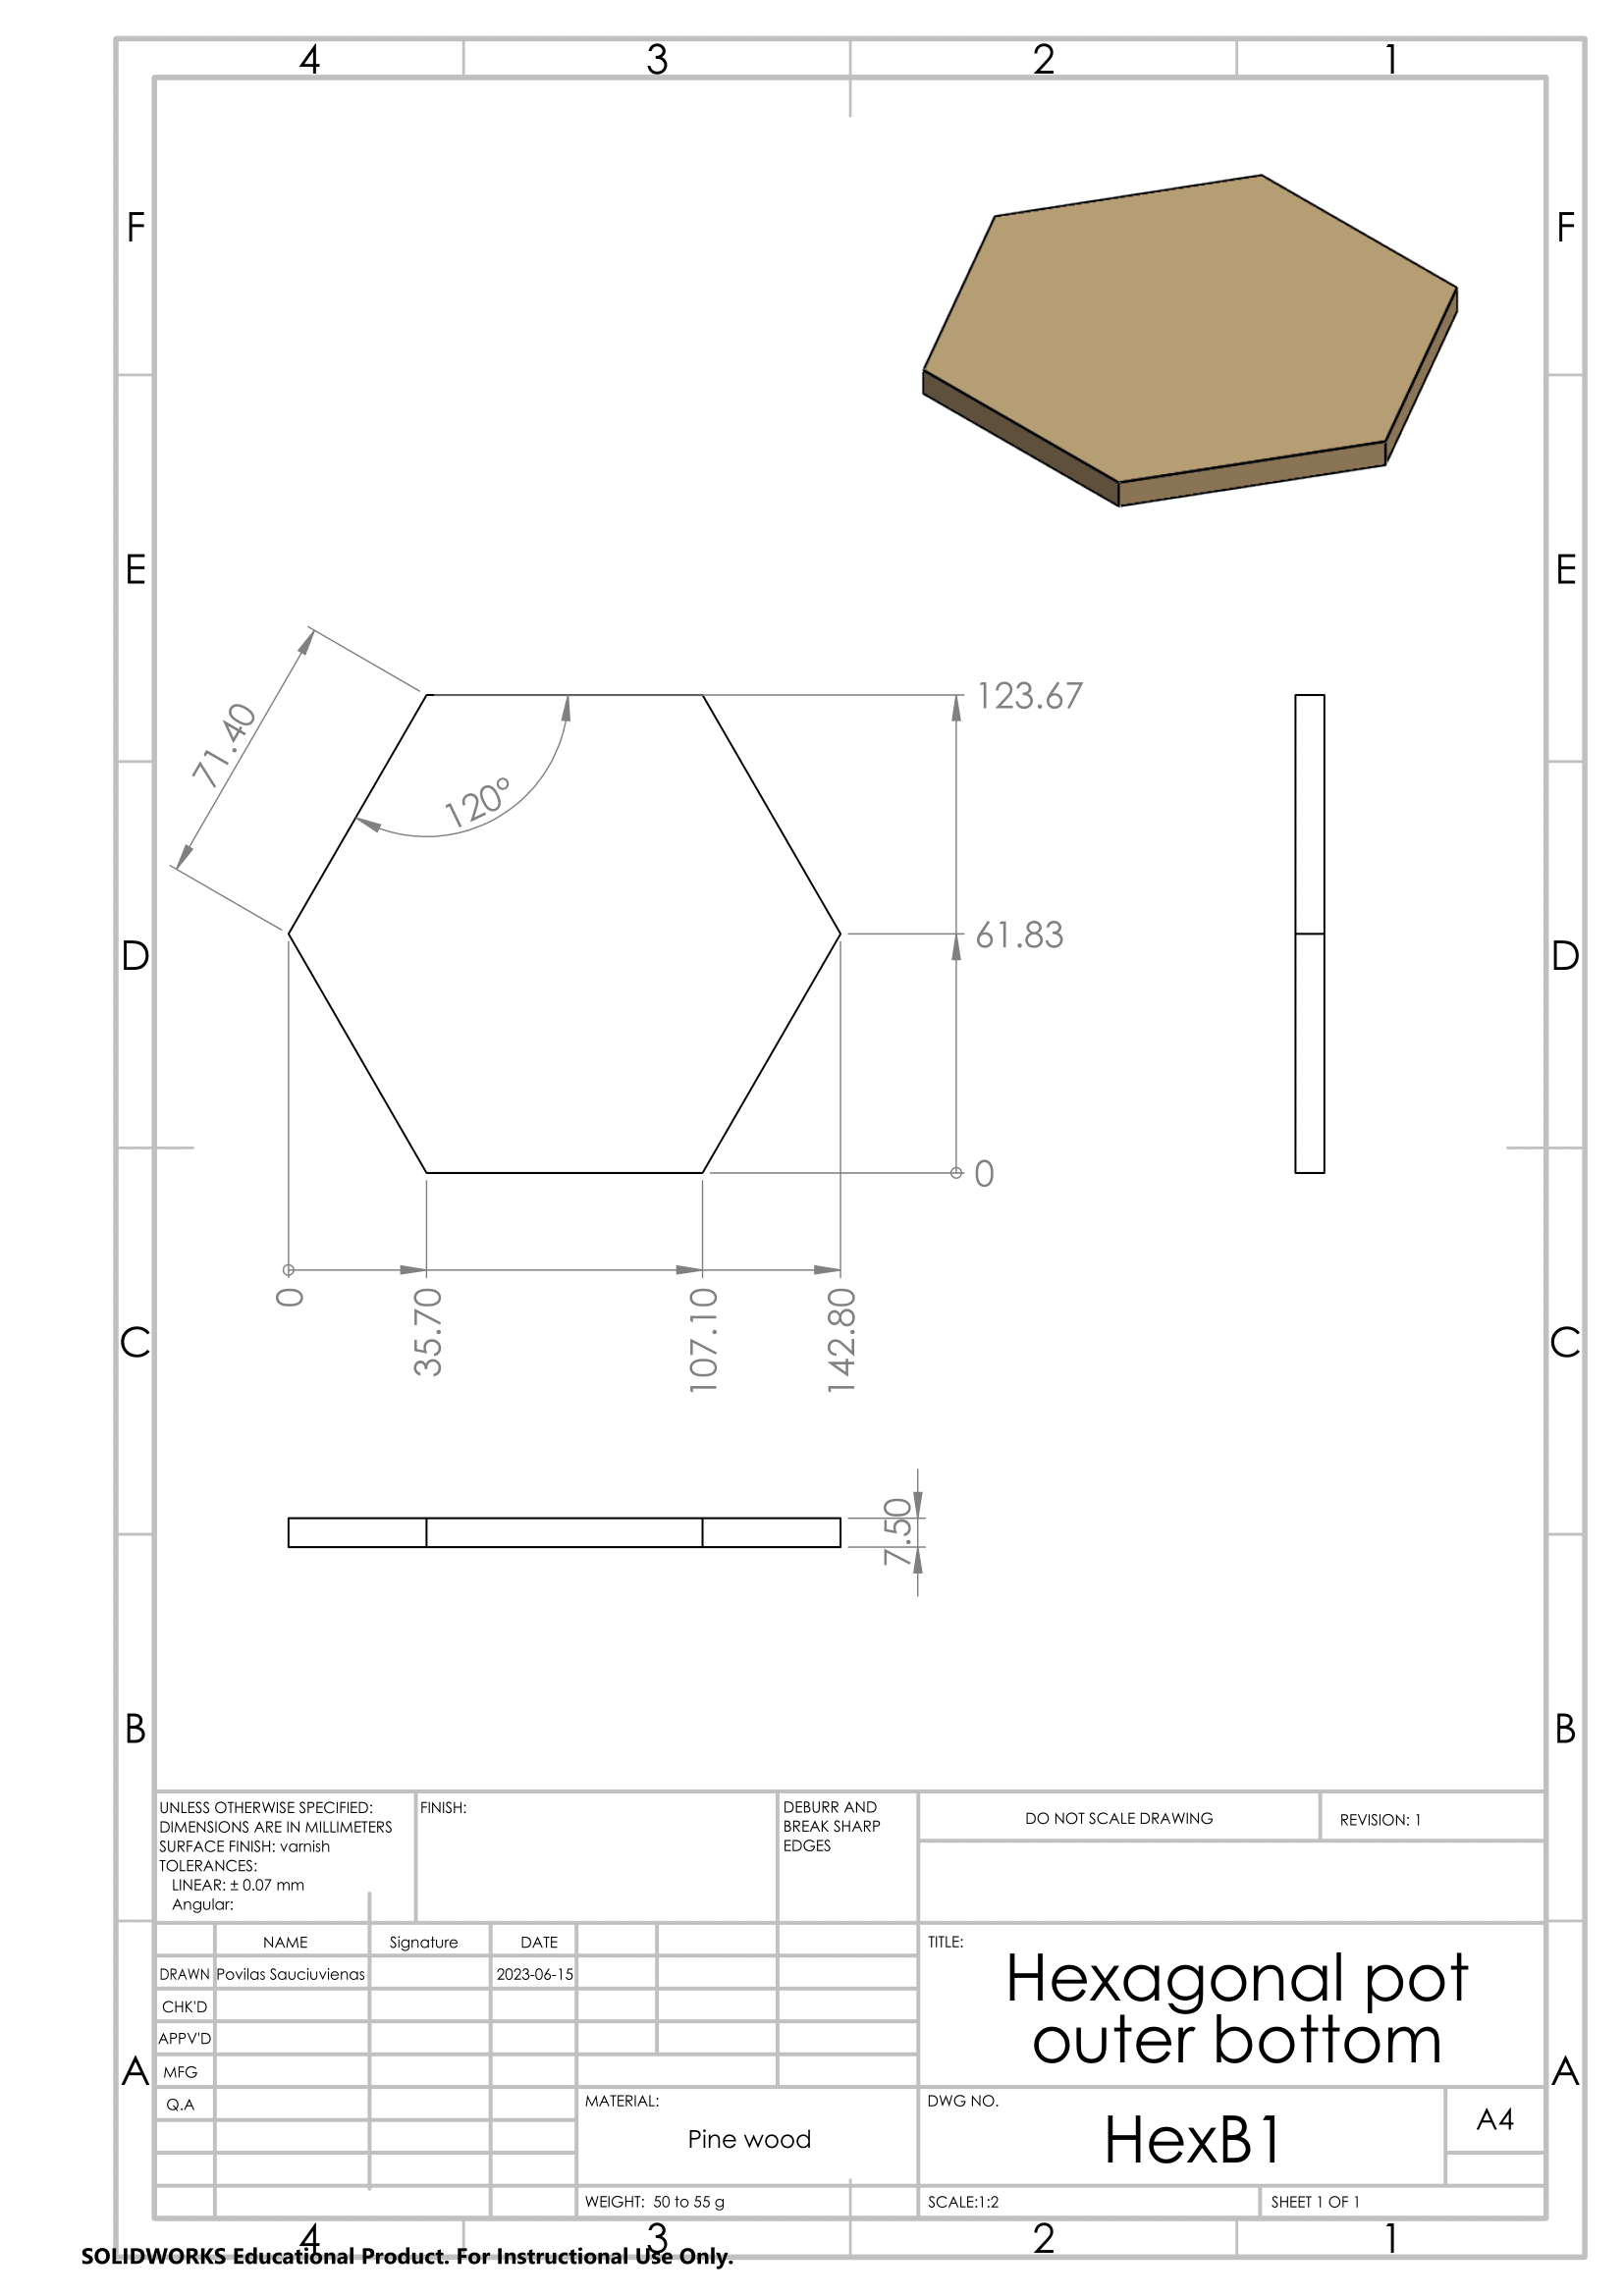
\includegraphics[width=0.9\textwidth]{images/technical_drawings/Hexagonal pot outer bottom-1.png}
    \caption{Technical drawing of the \textbf{outer bottom of the hexagonal pot} required for assembly explained in section \ref{topic:CNC_Milling}.}
    \label{technical_drawing:hex_pot_outer_bottom}
\end{figure}

% Pentagonal pot side part
\begin{sidewaysfigure}[!ht]
    \centering
    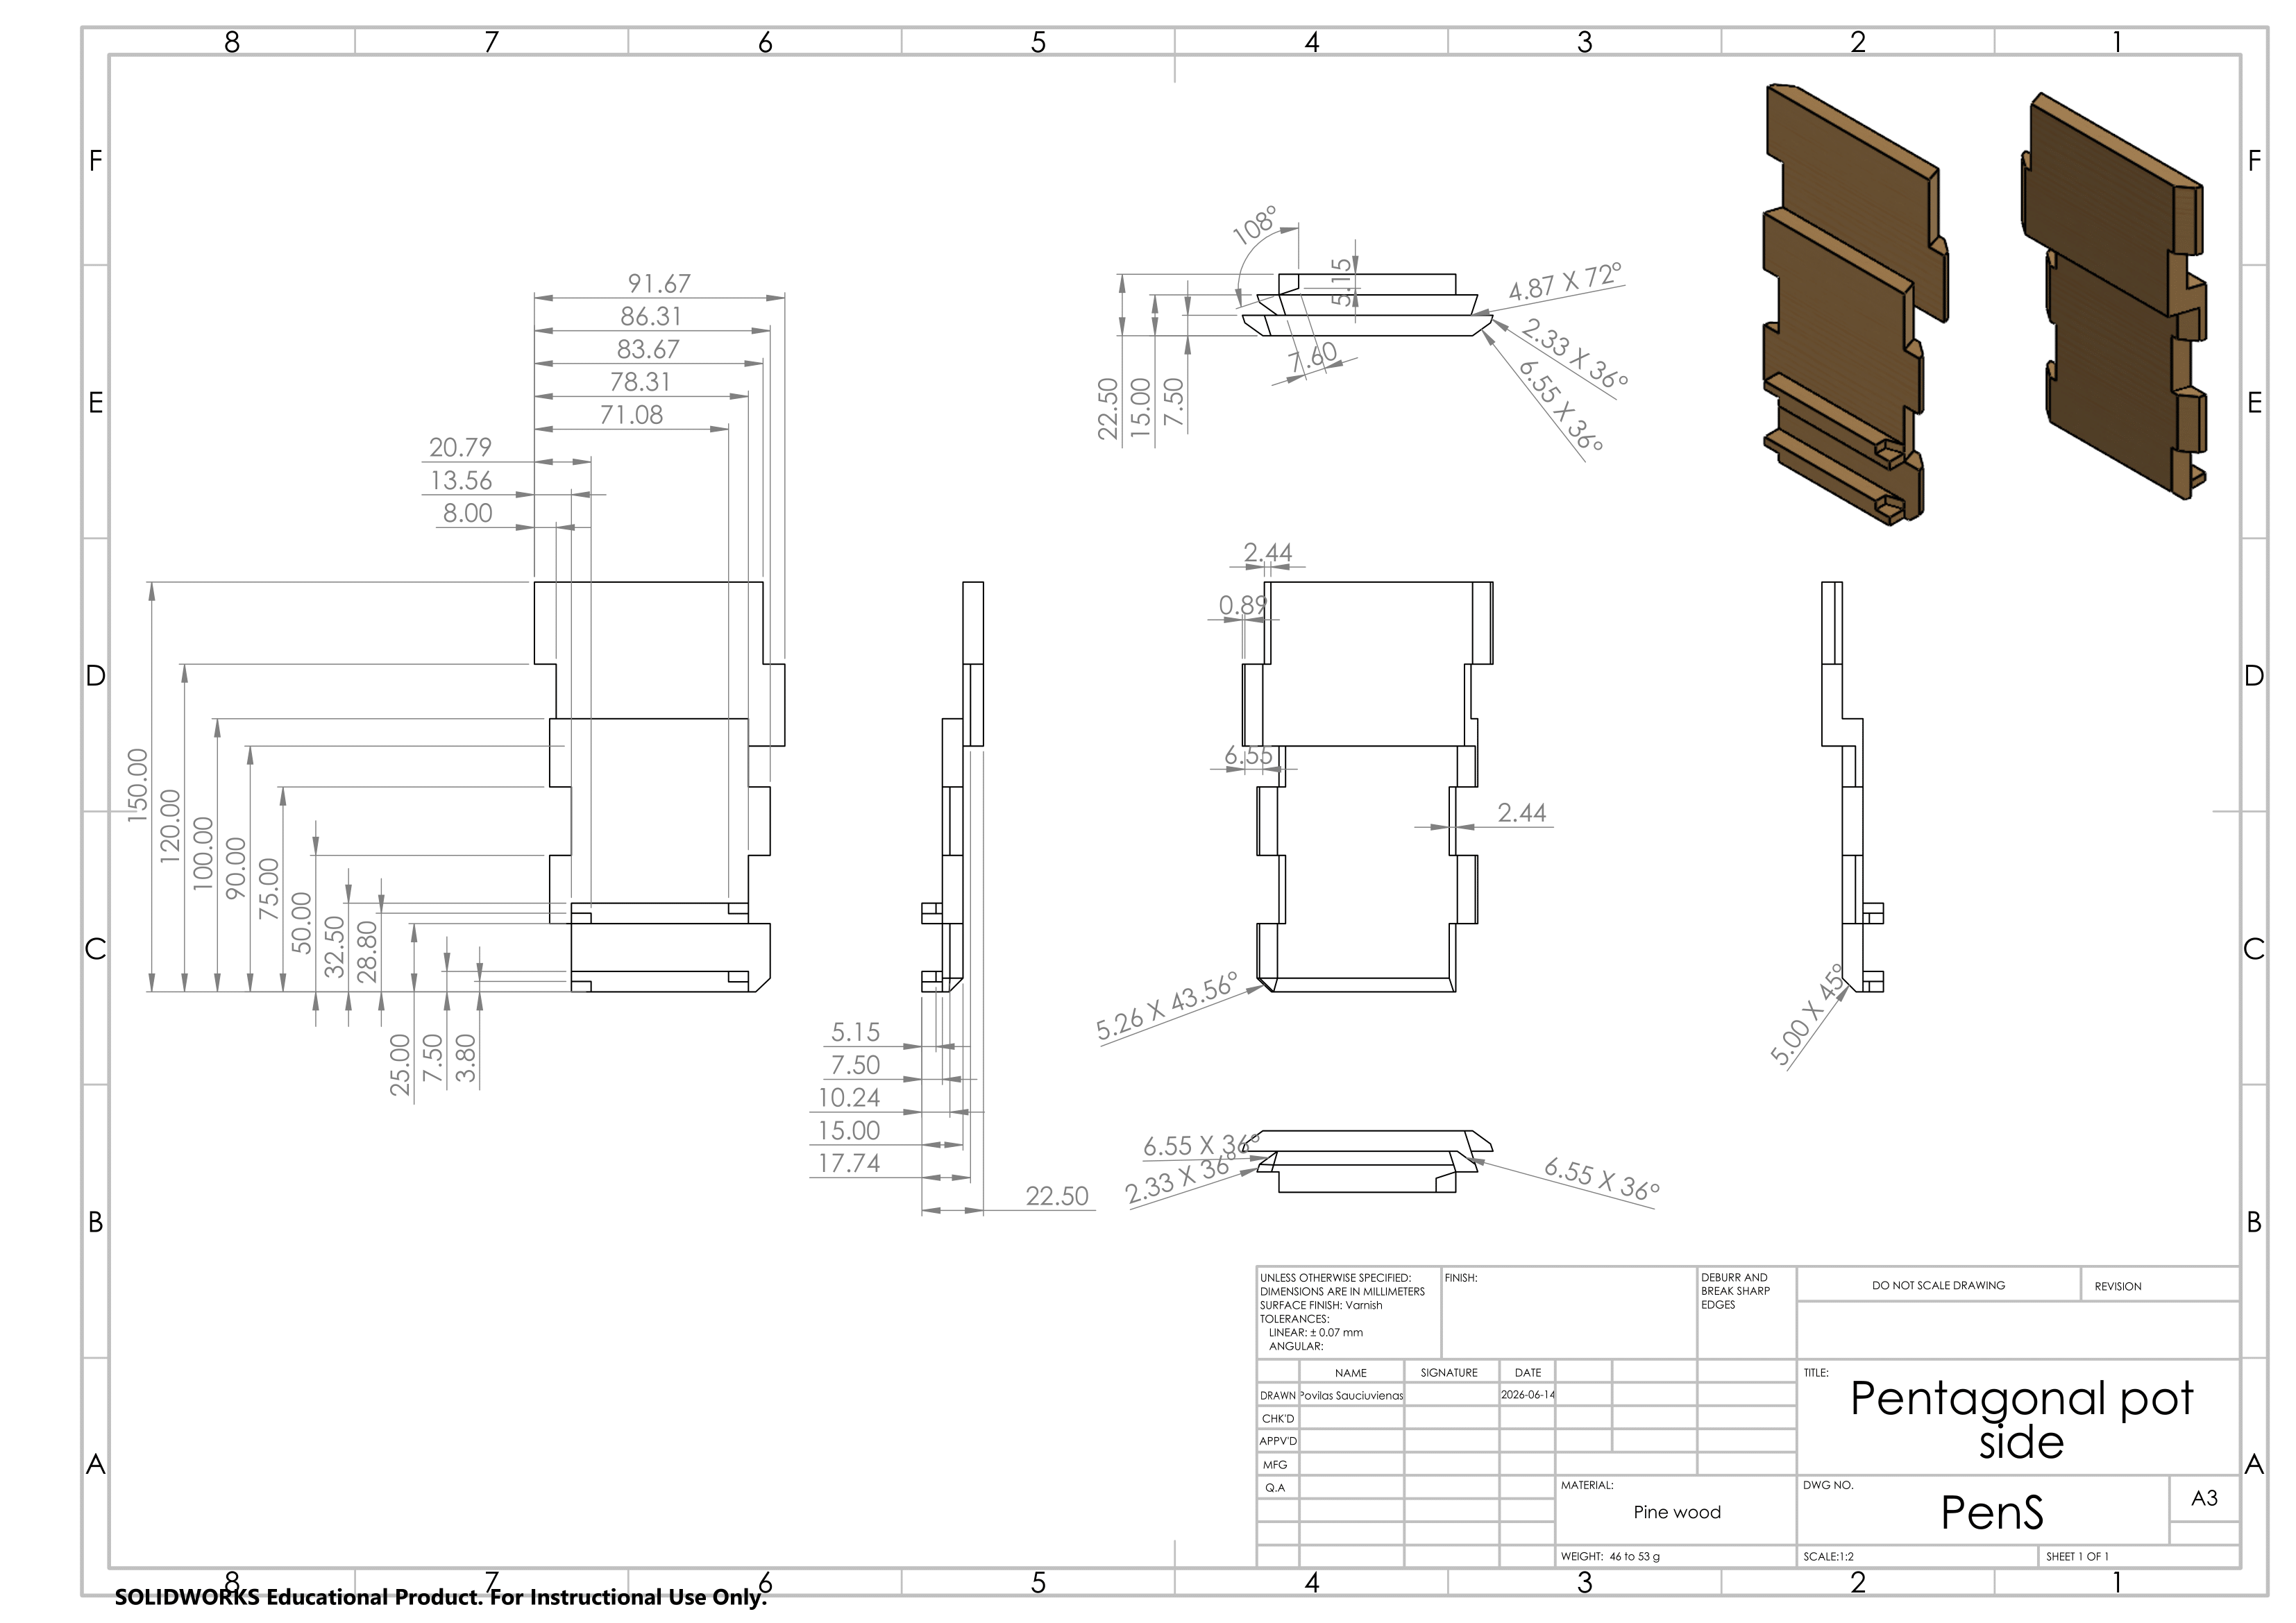
\includegraphics[width=1\textwidth ]{images/technical_drawings/Pentagonal side-1.png}
    \caption{Technical drawing of the \textbf{side part (one of six) of the pentagonal pot} required for assembly explained in section \ref{topic:CNC_Milling}.}
    \label{technical_drawing:pent_pot_side_part}
\end{sidewaysfigure}

% Pentagonal pot inner bottom
\begin{figure}[ht]
    \centering
    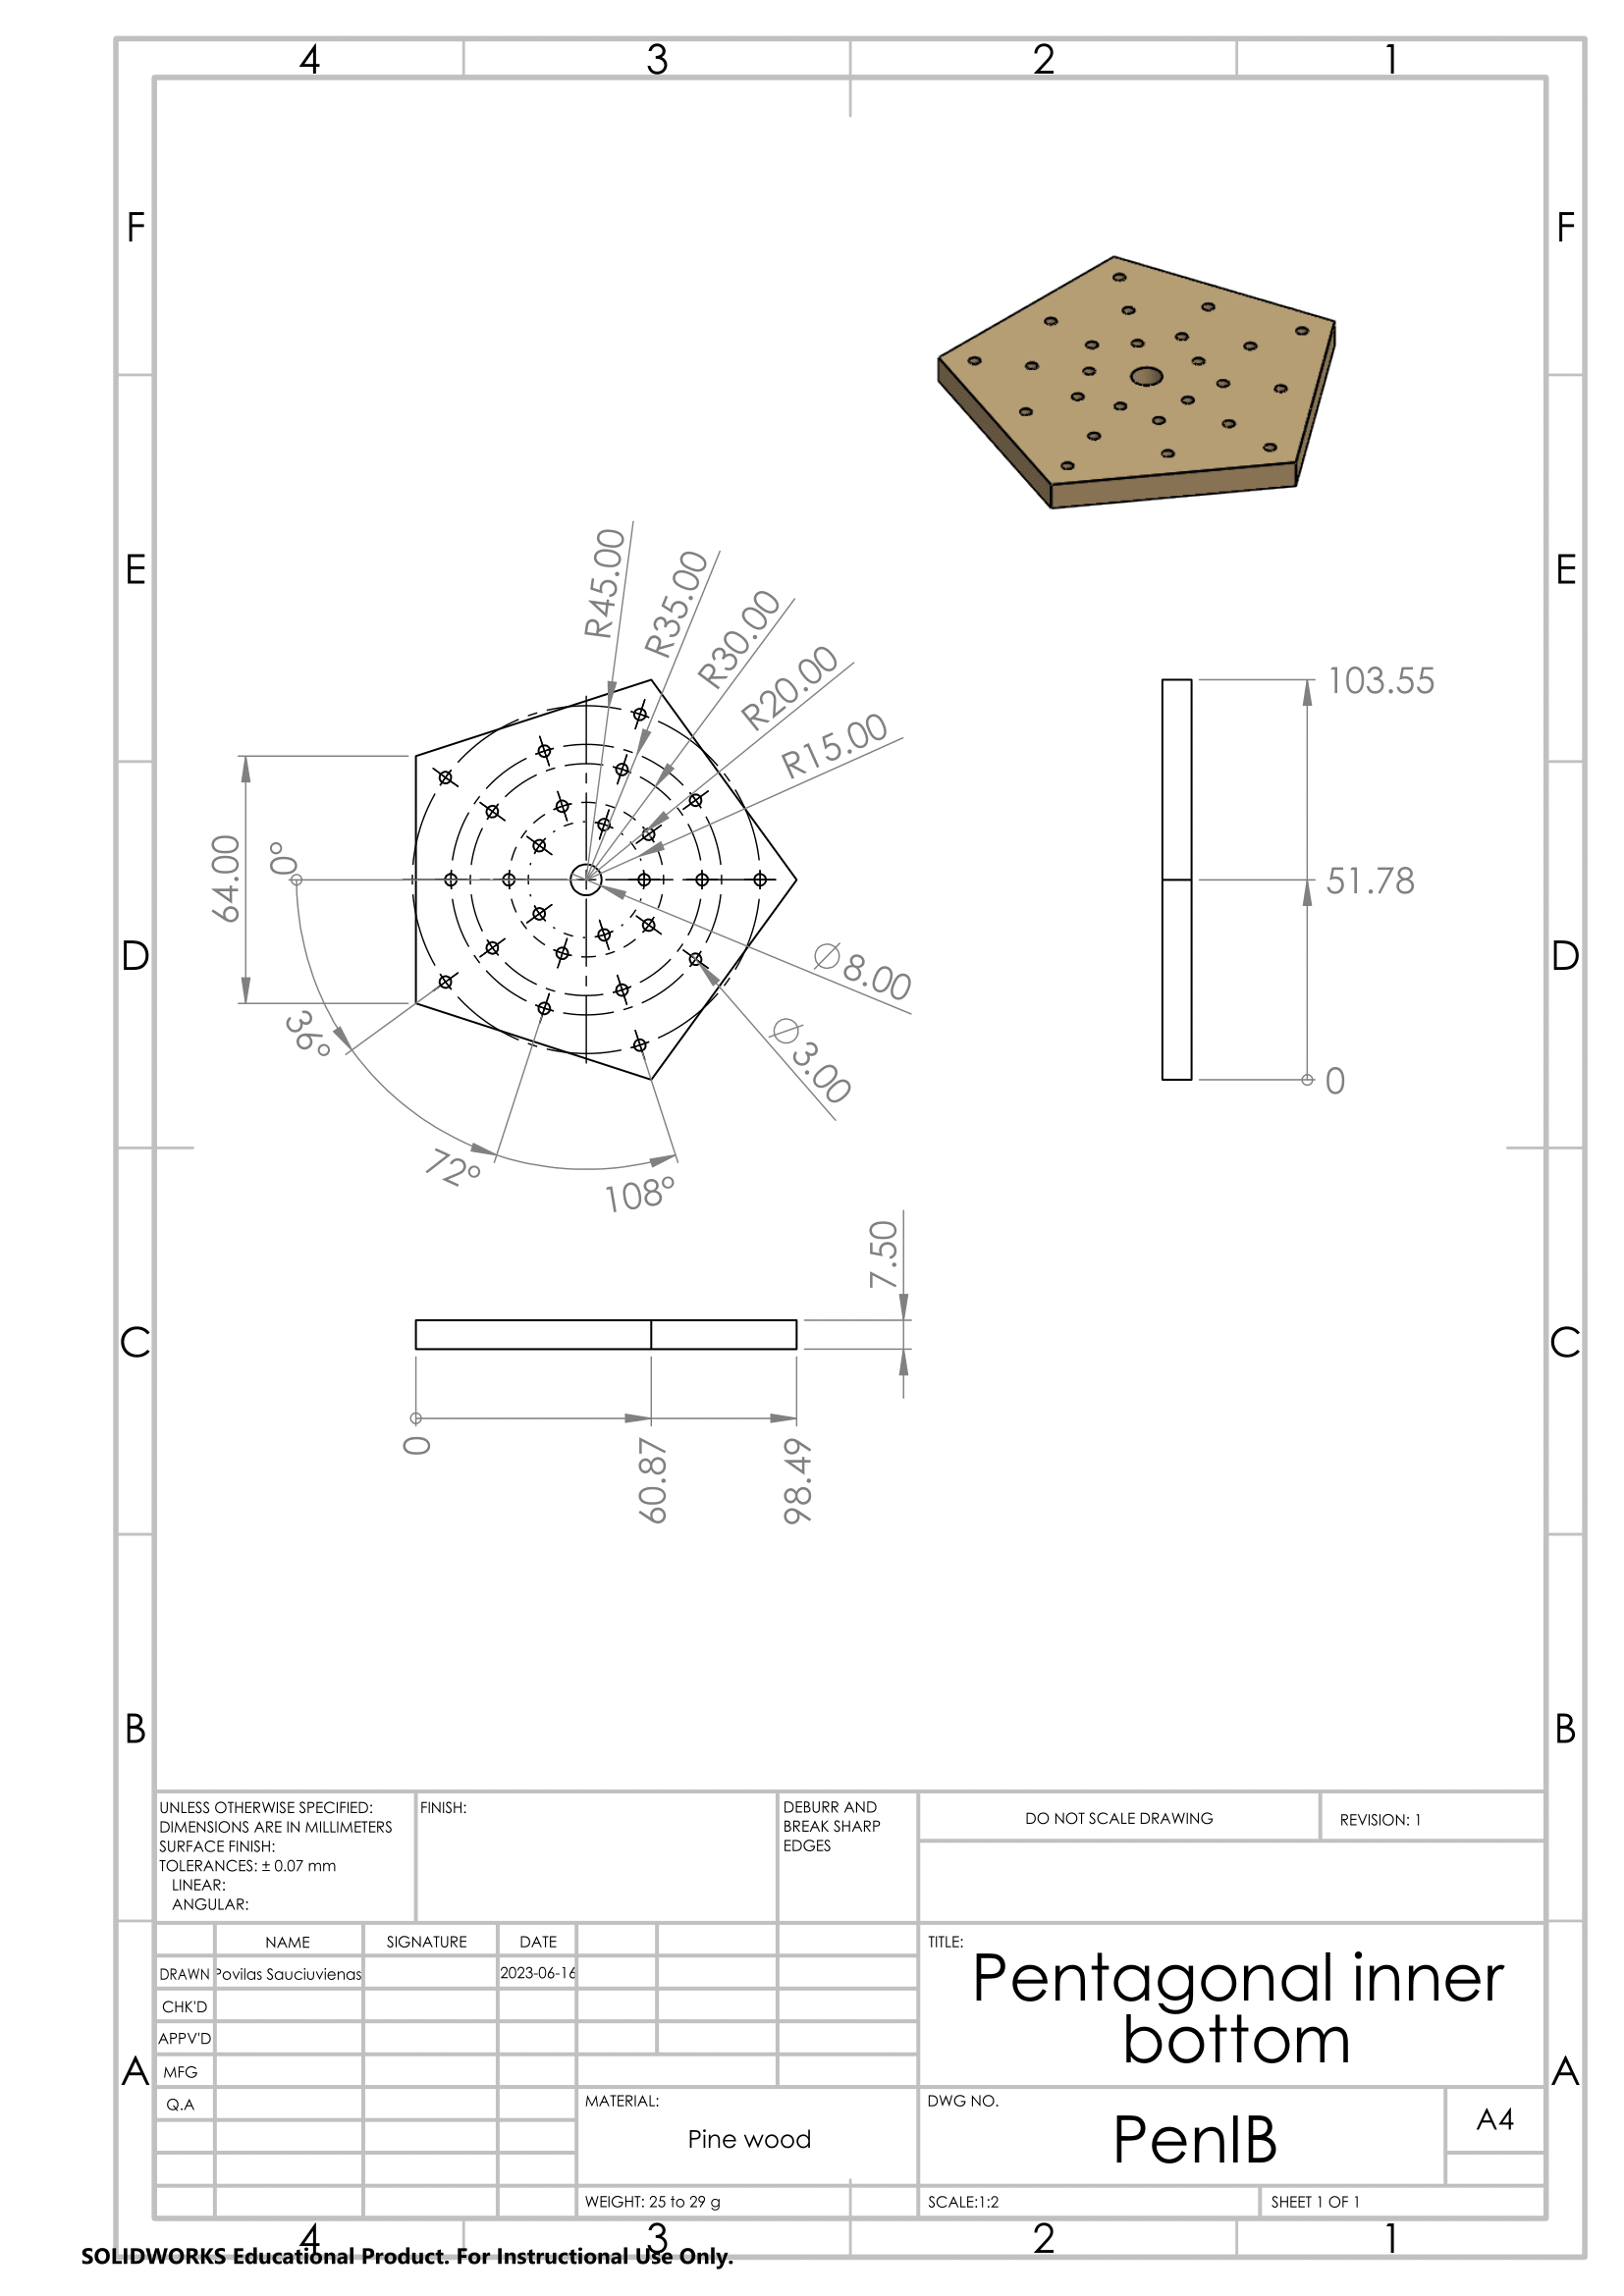
\includegraphics[width=0.9\textwidth]{images/technical_drawings/Pentagonal inner bottom-1.png}
    \caption{Technical drawing of the \textbf{inner bottom of the pentagonal pot} required for assembly explained in section \ref{topic:CNC_Milling}.}
    \label{technical_drawing:pent_pot_inner_bottom}
\end{figure}

% Pentagonal pot outer bottom
\begin{figure}[ht]
    \centering
    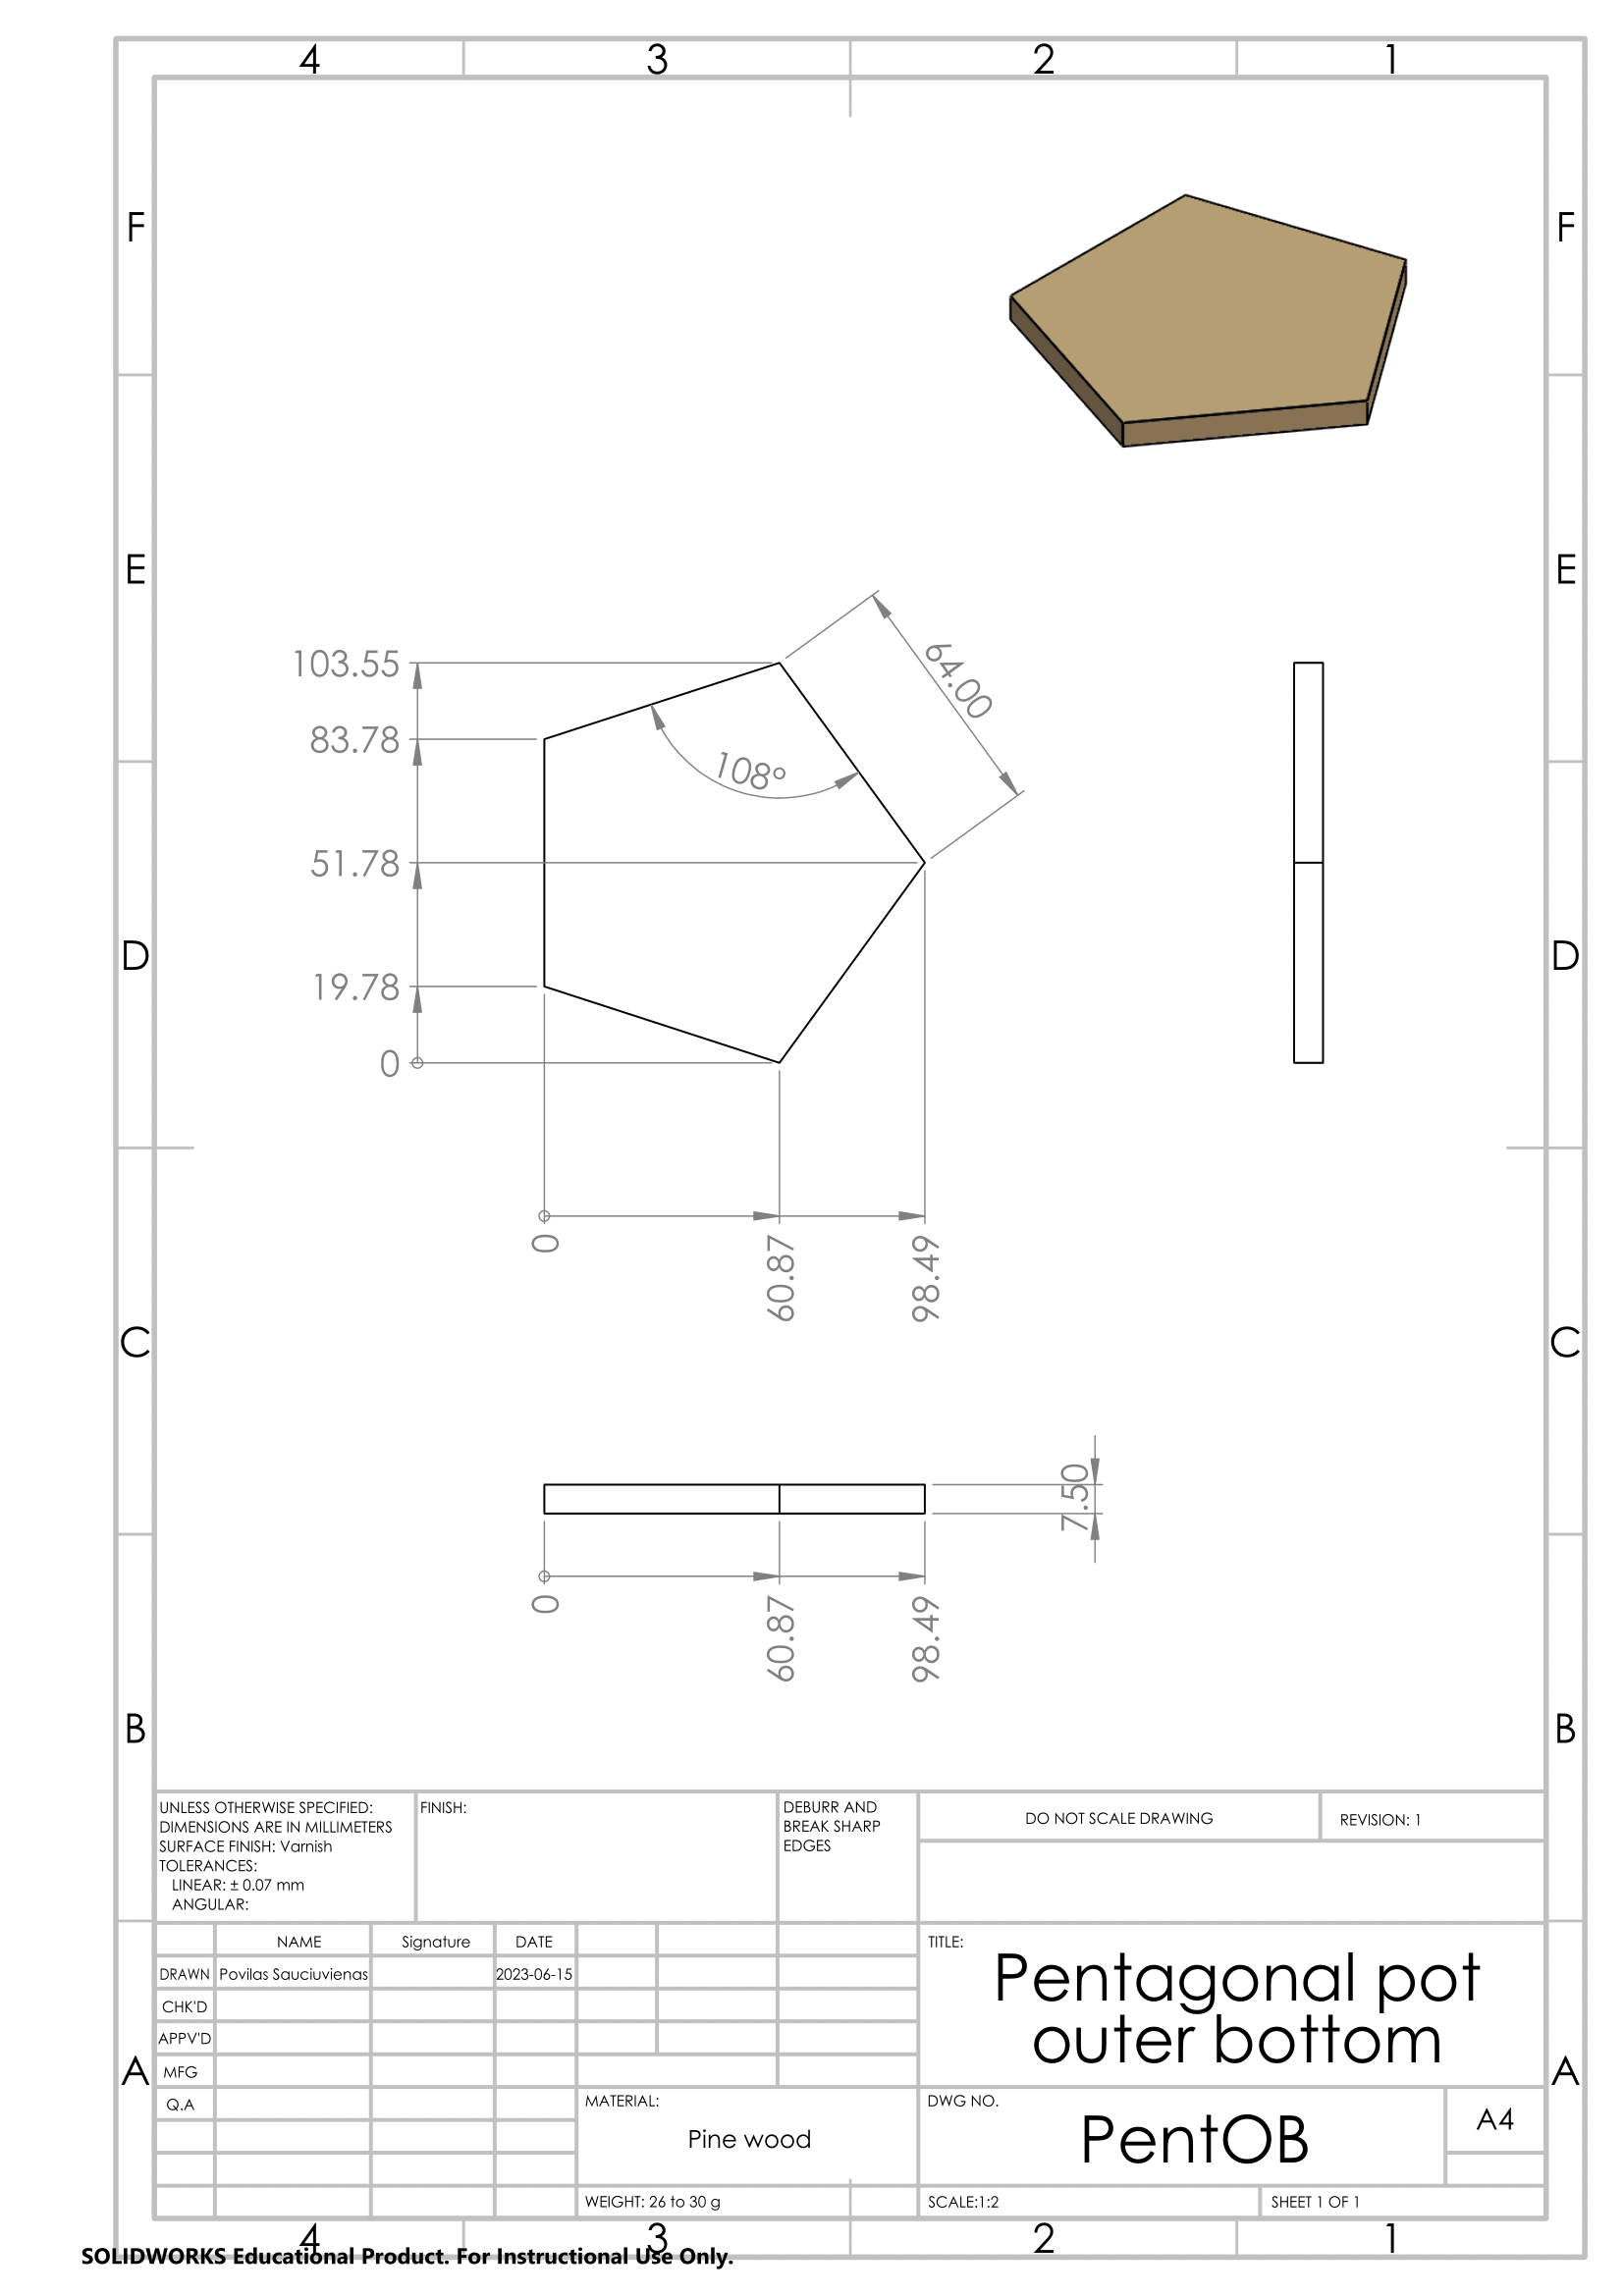
\includegraphics[width=0.9\textwidth]{images/technical_drawings/Pentagonal pot outer bottom-1.png}
    \caption{Technical drawing of the \textbf{outer bottom of the pentagonal pot} required for assembly explained in section \ref{topic:CNC_Milling}.}
    \label{technical_drawing:pent_pot_outer_bottom}
\end{figure}
\pagebreak
%\begin{figure}[ht]
 %   \centering
  %  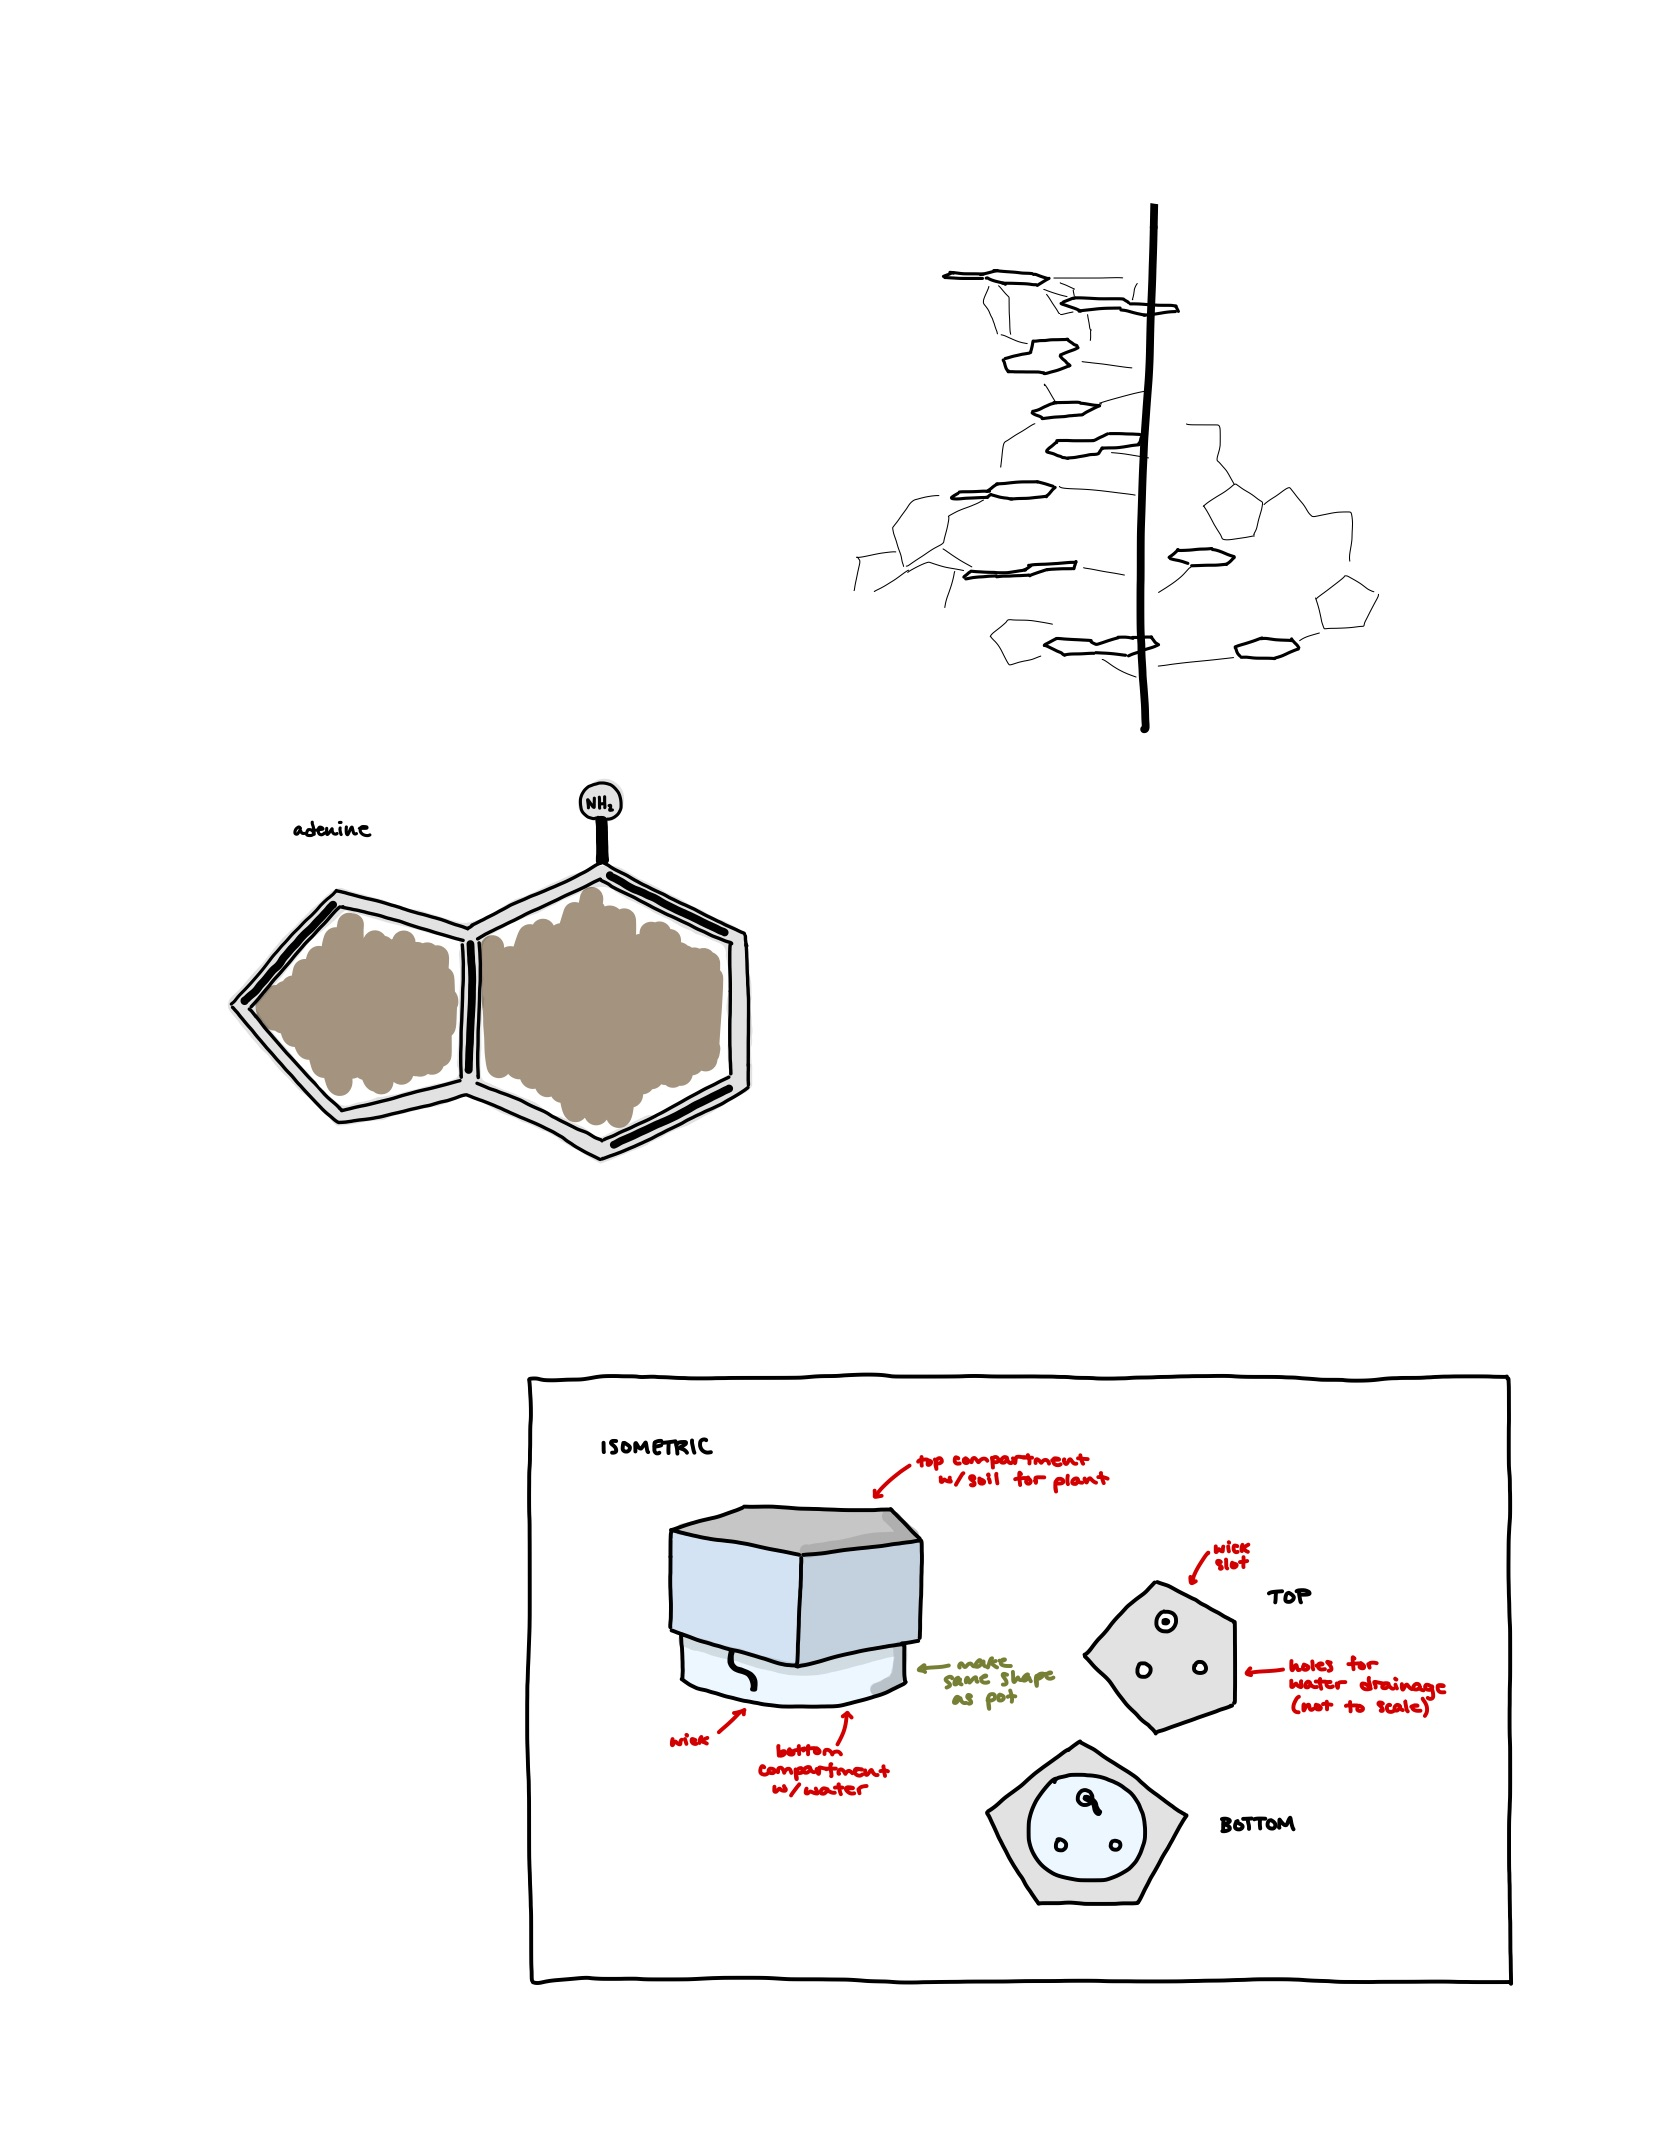
\includegraphics[scale=0.5]{images/Drawings/design drawings.jpg}
   % \caption{Caption}
    %\label{fig:design_drawings}
%\end{figure}
%\begin{figure}[ht]
 %   \centering
  %  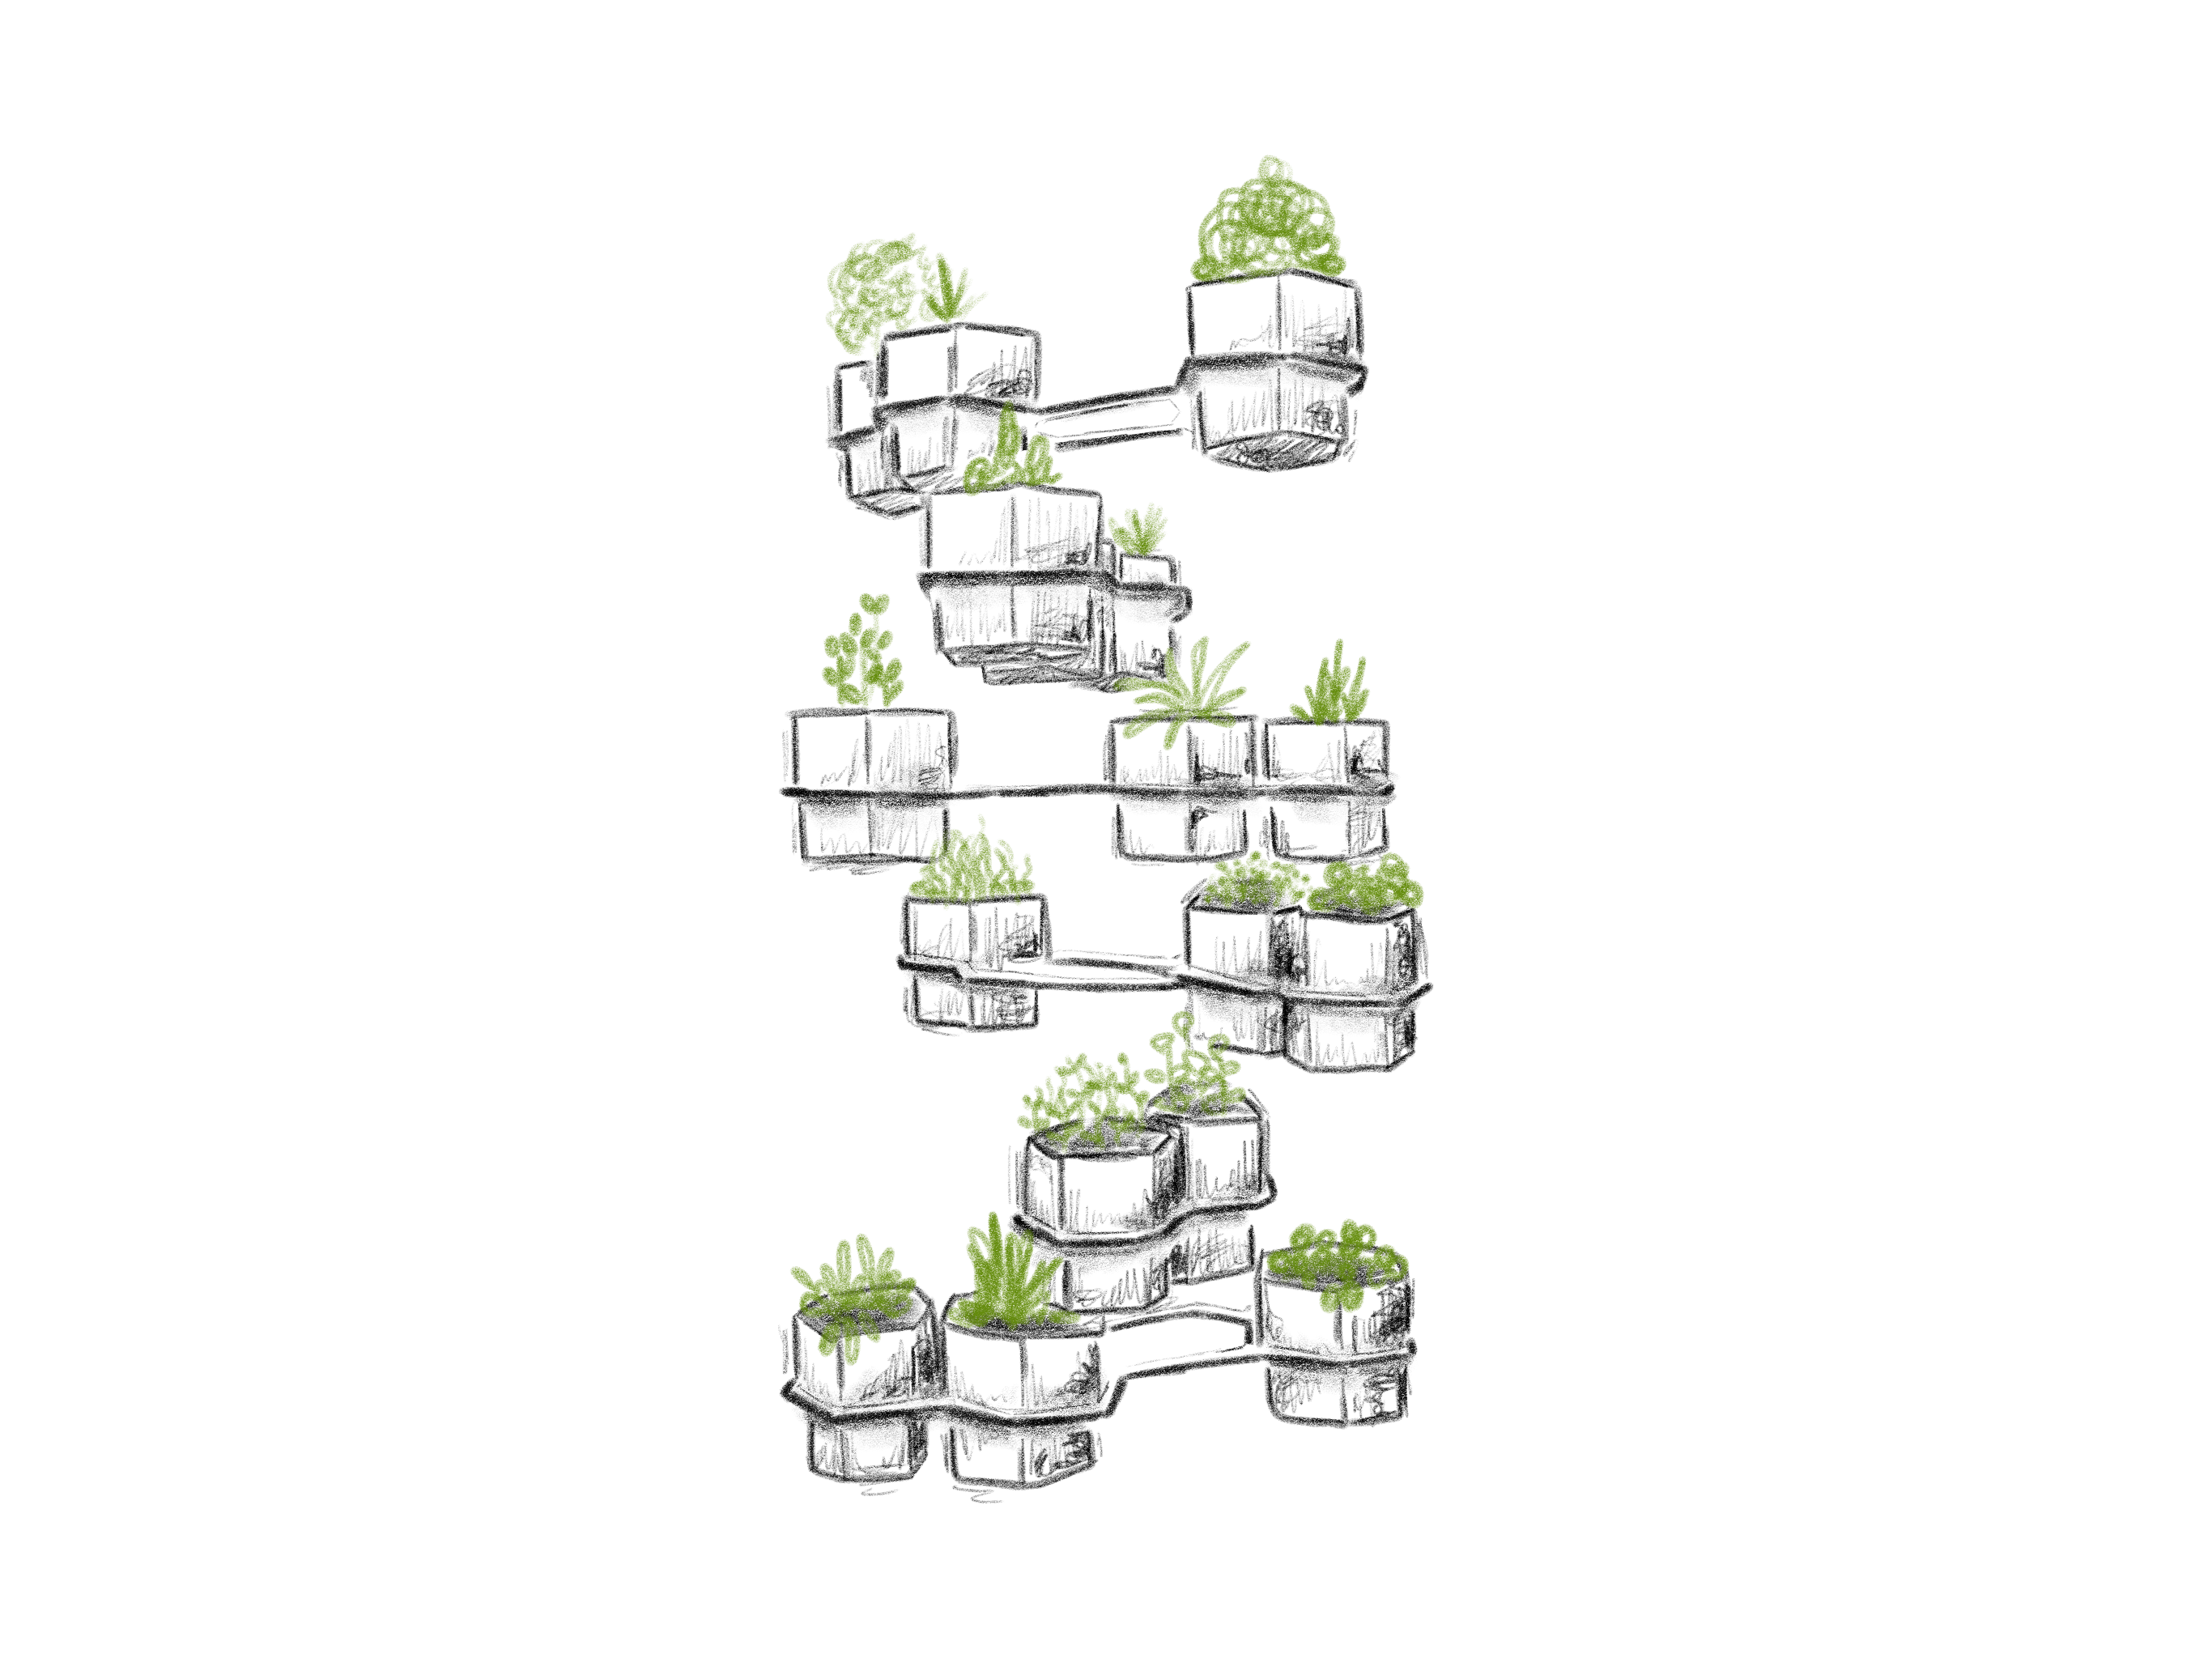
\includegraphics[scale=0.2]{images/Drawings/fullstructure.png}
   % \caption{Caption}
   % \label{fig:drawing_fullstructure}
%\end{figure}
%\pagebreak
\begin{figure}[ht]
    \centering
    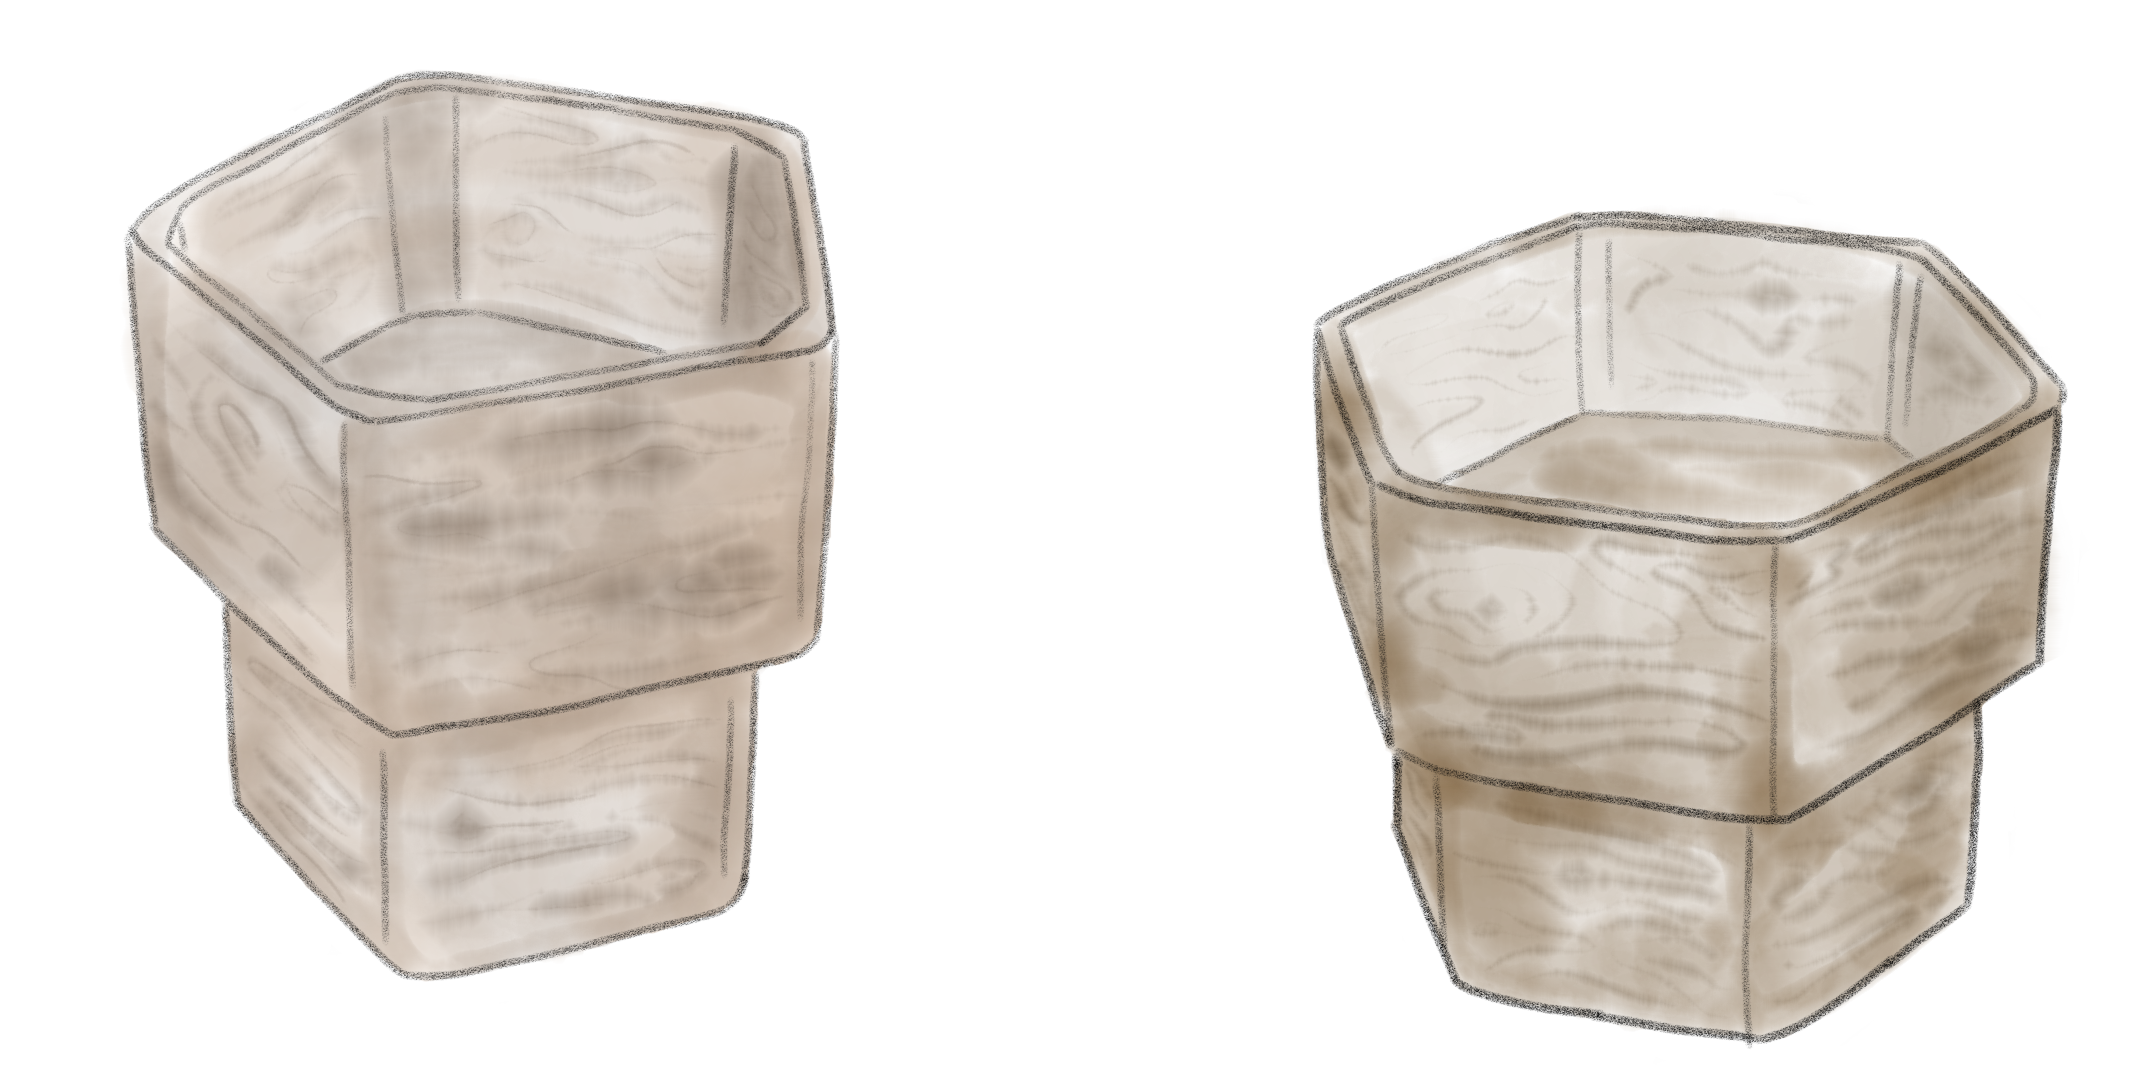
\includegraphics[scale=0.2]{images/Drawings/pot drawings.png}
    \caption{Drawing of the two types of pots.}
    \label{fig:pot_drawings}
\end{figure}
\begin{figure}[ht]
    \centering
    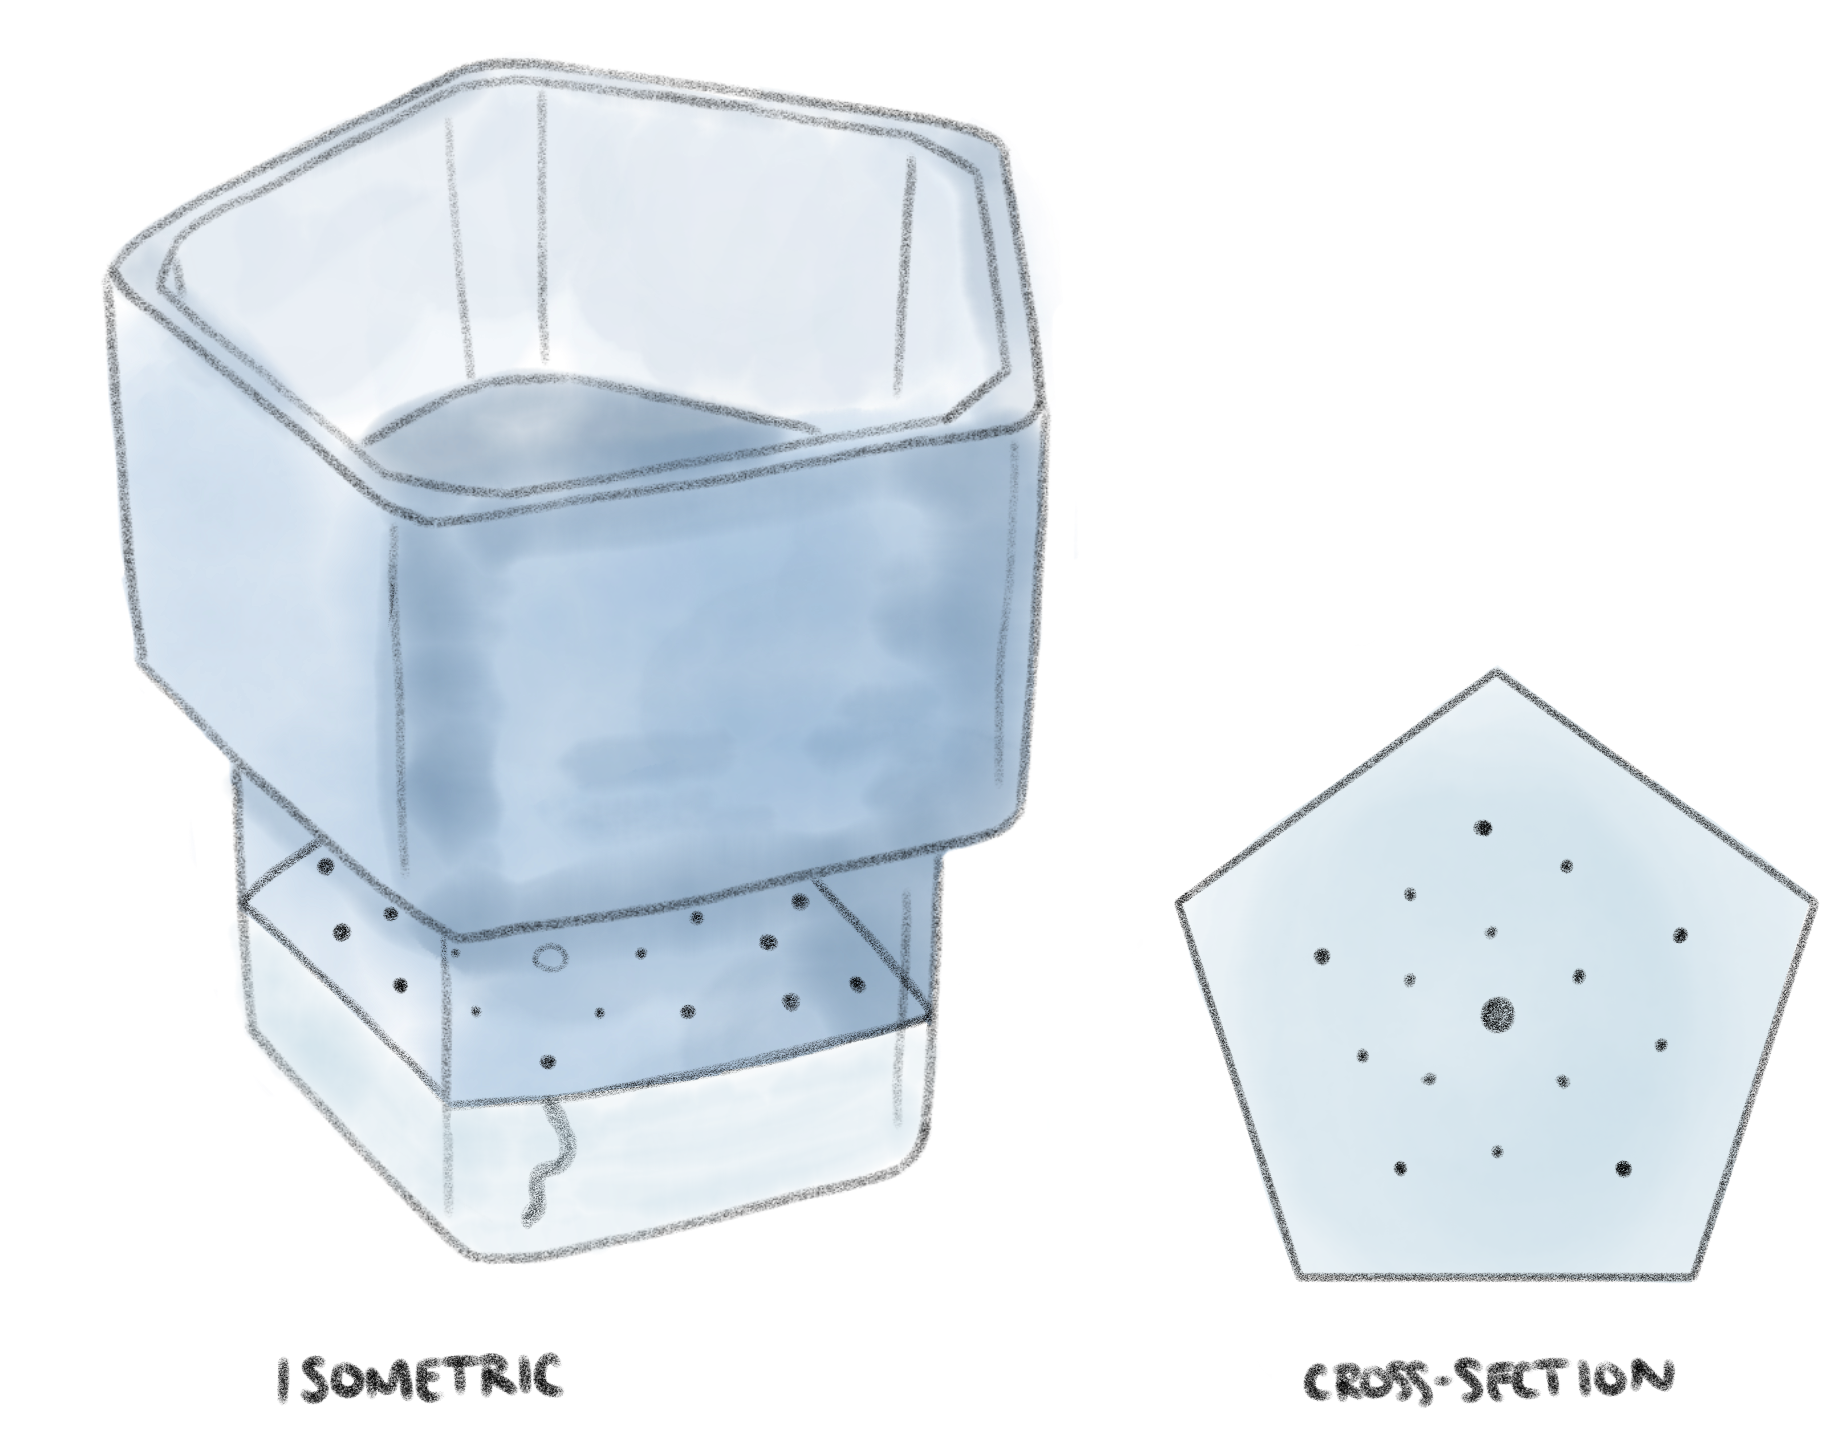
\includegraphics[scale=0.2]{images/Drawings/wick system.png}
    \caption{Drawing of the wick system.}
    \label{fig:wick_system}
\end{figure}
\end{document}
